%# -*- coding: utf-8-unix -*-
%%==================================================
%% thesis.tex
%%==================================================

% 双面打印
\documentclass[master, fontset=adobe, openright, twoside, zihao=-4]{sjtuthesis}
% \documentclass[bachelor, fontset=adobe, openany, oneside, submit]{sjtuthesis}
% \documentclass[master, fontset=adobe, review]{sjtuthesis}
% \documentclass[%
%   bachelor|master|doctor,	% 必选项
%   fontset=adobe|windows,  	% 只测试了adobe
%   oneside|twoside,		% 单面打印,双面打印(奇偶页交换页边距,默认)
%   openany|openright, 		% 可以在奇数或者偶数页开新章|只在奇数页开新章(默认)
%   zihao=-4|5,, 		% 正文字号:小四、五号(默认)
%   review,	 		% 盲审论文,隐去作者姓名、学号、导师姓名、致谢、发表论文和参与的项目
%   submit			% 定稿提交的论文,插入签名扫描版的原创性声明、授权声明 
% ]

% 逐个导入参考文献数据库
\addbibresource{bib/thesis.bib}
% \addbibresource{bib/chap2.bib}

\begin{document}

%% 无编号内容:中英文论文封面、授权页
%# -*- coding: utf-8-unix -*-
\title{基于容器的主动式云负载均衡技术}
\author{吴\quad{}晔}
\advisor{梁阿磊副教授}
\coadvisor{陈昊鹏副教授}
\defenddate{2018年1月10日}
\school{上海交通大学}
\institute{电子信息与电气工程学院}
\studentnumber{115037910017}
\major{软件工程}

\englishtitle{Proactive Load Balancing in Container-based Cloud}
\englishauthor{\textsc{Ye Wu}}
\englishadvisor{Associate Professor \textsc{Alei Liang}}
\englishcoadvisor{Associate Professor \textsc{Haopeng Chen}}
\englishschool{Shanghai Jiao Tong University}
\englishinstitute{\textsc{School of Software} \\
  \textsc{Shanghai Jiao Tong University} \\
  \textsc{Shanghai, P.R.China}}
\englishmajor{A Very Important Major}
\englishdate{Jan. 10th, 2018}


\maketitle

\makeenglishtitle

\makeatletter
\ifsjtu@submit\relax
	\includepdf{pdf/original.pdf}
	\cleardoublepage
	\includepdf{pdf/authorization.pdf}
	\cleardoublepage
\else
\ifsjtu@review\relax
% exclude the original claim and authorization
\else
	\makeDeclareOriginal
	\makeDeclareAuthorization
\fi
\fi
\makeatother


\frontmatter 	% 使用罗马数字对前言编号

%% 摘要
\pagestyle{main}
%# -*- coding: utf-8-unix -*-
%%==================================================
%% abstract.tex for SJTU Master Thesis
%%==================================================

\begin{abstract}
随着云计算在过去十年间的发展,越来越多的软件厂商和软件服务提供商选择将业务迁移到云平台中以降低自身的运营维护成本。容器虚拟化技术作为云计算的另一种实现方式,由于其轻量、高效的特性在过去几年备受云计算厂商的关注和青睐,Docker作为目前最受欢迎的容器虚拟化平台,由于其提出的Docker镜像机制而被广泛应用于容器云中充当基础平台。于此同时,随着互联网的爆发和普及,突发性的负载变化越来越成为常态。虽然容器云用户可以通过设定阈值的方式通过监控负载状态进行服务的自动伸缩,但是这些调整都只能被动地相应负载的变化,除了滞后于实际负载变化外还需要依赖用户根据主观的方式来设定阈值。除此之外,目前用于构建容器云的容器集群框架中并没有合理服务的可用性需求和负载需求,只是单纯地利用服务的实例数来统一应对服务的可用性需求和负载要求。在应对负载变化方面,现有的容器集群框架也更多的关注于对应用或者服务的负载均衡,在负载迅速变化的场景下缺乏相应的任务调度和管理机制,从而无法快速响应变化的负载。

为了应对如今越来越复杂的负载环境,本文提出了一个基于容器的主动式云资源管理模型,着重解决在满足可用性指标的前提下,通过对负载进行预测来提前对服务进行调整,根据预测的结果主动对服务进行调整以应对负载的变化,减少用户手动的调节设置;利用容器镜像的特性使容器云快速响应负载的变化,从而更好地应对现实中激烈多变的负载,在保证容器云中服务的服务质量的同时降低了容器云供应商的成本。

本文将内存、CPU时间、磁盘和网络带宽等资源的使用量和使用率作为负载的衡量,对系统进行实时的监测,从而获得系统实时的负载状态。随后根据历史资源使用状态监测数据,通过使用相应的预测模型对资源使用状态进行预测,给出未来一段时间内的资源使用量的预测值。

在获得预测到的资源使用状态之后,本文通过模型中的资源供给方案生成模块将相应的资源使用量转化成相应服务需要的实例数。由于预测本身不能保证完全的准确,我们在模型中通过资源供给优化模块根据实时的资源使用状态对服务实例规模进行调整。资源管理模块会基于满足服务可用性要求所需要的副本数,分别根据基于预测和实际监测得到的实例数确认最终进行调整的任务实例规模。

在确认了最终需要调整的服务实例规模之后,本文提出的模型通过负载优化模块利用服务伸缩的方法进行实际的调整。本文利用Docker镜像的层级文件系统和内容寻址特性,提出一个基于层级文件缓存的启发式调度算法。根据当前容器云中所有节点的资源分配状态和目标服务的限制选择合适的节点来托管相应任务实例,通过分析服务中任务实例的分布状态,利用节点上的Docker镜像层级文件缓存以减少依赖环境的下载和安装的耗时,从而降低了服务伸缩操作的延迟,达到在保证服务可用性的基础上提升响应速度的目标。

最后,本文为了验证模型的有效性设计了相关实验。实验结果证明,本课题使用的预测模型可以为主动性调整提供一个相对可靠的预测结果;在负载急剧增加的场景下,和Docker \emph{swarm}框架相比,本文提出的模型显著加快了服务在容器云中的扩展速度;而在负载降低的场景下,本文提出的模型保证了服务收缩的操作和Docker \emph{swarm}框架中的服务收缩操作一样高效;在对服务的实例规模进行调整的过程中,服务的样本规模始终保证满足设定的副本数目标。从所有的实验结果可以看出本文提出的模型在负载变化的环境下可以提升容器云对变化负载的应对能力和服务调整的灵活性。

\keywords{\large 容器云 \quad 负载变化 \quad 负载预测 \quad Docker镜像 \quad 集群管理和调度}
\end{abstract}

\begin{englishabstract}
With the development of cloud computing in the last ten years, there more and more software producers and service providers trying to mitigate their services from traditional clusters to clouds for lower costs and other benefits brought by virtualization. Containerization is becoming increasingly popular in virtualization nowadays and Docker is one of the most popular container platforms to deploy and manage applications. Docker introduces Docker image which is considered as the basement of container-based clouds. Besides, as the internet is widely spread and in common use, load varies more dynamically and more intensively. Whereas cloud users can use certain tools, provided by cloud providers, to scale services automatically by setting some thresholds, the adjustment always lags behind the load changes and depends on subjective estimation. What's more, the definition of replica is equivalent to the number of instances in all container cluster frameworks, which are used as the infrastructure of container-based clouds. The lack of suitable scheduling policy and management mechanism in these frameworks makes services difficult to cope with dynamic load changes.

Fast startup and spread of services provides services the ability of reacting to bursting load changes rapidly. In this paper, we introduce a proactive load optimizer model in container-based cloud to accelerate the process of service creation and spread in container-based clouds to cope with dynamic load changes. The models makes scale decisions in advance, depending on load predictions according to history data. What's more, the model leverages caches from Docker image filesystems to speed up the creation and spread of services in container clouds, under the promise of meeting their availability requirements.

In the model, we monitor the resources usage status, such as memory, cpu time and network bandwidth, etc.. We take these resource usage status as the measurements of real-time loads. Later, we use certain prediction models to predicate the resource usages in the next periods according to history monitor data.

Provision module is used to get the accurate number of instances accroding to resource usage predictions in the model. As predictions have no accuracy promises for the actual load changes, we use optimization module to adjust the scale when real-time load is out of some thresholds. After all, management module is used to make the final decisions about the scales of corresponding services accroding to their replica requirements.

In the scheduling module, the service will be scaled according to the confirmed size. In the model, we introduce a heuristic scheduling algorithm, which leverages the layered file system in Docker image and the feature of content addressability, to make final scheduling decisions for services, in consideration of replica distributions, reusable buffered layers and resource allocations. In the algorithm, we try to minimise the time cost during the download and installation of dependency packages and environments to speed up the process of service creation and service scaling.

Finally, we design some experiments to validate the model. The accuracy of predications for load changes in the model is acceptable.By comparing the model with Docker swarm, the results show that it's much faster to create a service and scale out a service with the help of the model. The time consumption of scaling in a service is almost the same in both Docker swarm and the model. We introduce a new constraint as replica to assure services not violating their replica requirements with the model. All of the results show that the model has a better performance for services in container-based clouds with dynamically varying loads.

\englishkeywords{\large Container-based Cloud, Docker Image, Load Changes, Load Prediction, Cluster Scheduling}
\end{englishabstract}


%% 目录、插图目录、表格目录
\tableofcontents
\listoffigures
\addcontentsline{toc}{chapter}{\listfigurename} %将插图目录加入全文目录
\listoftables
\addcontentsline{toc}{chapter}{\listtablename}  %将表格目录加入全文目录
\listofalgorithms
\addcontentsline{toc}{chapter}{算法索引}        %将算法目录加入全文目录

% \include{tex/symbol} % 主要符号、缩略词对照表

\mainmatter	% 使用阿拉伯数字对正文编号

%% 正文内容
\pagestyle{main}
%# -*- coding: utf-8-unix -*-
%%==================================================
%% chapter01.tex for SJTU Master Thesis
%%==================================================

%\bibliographystyle{sjtu2}%[此处用于每章都生产参考文献]
\chapter{绪论}
\label{chap:intro}

\section{研究背景和研究意义}\label{sec:intro_bg}
云计算在过去十年中备受欢迎,并被广泛应用到实际使用中,大量的云计算平台例如Amazon Web Services(AWS)\footnote{https://aws.amazon.com}、阿里云\footnote{https://www.aliyun.com}和Microsoft Azure\footnote{https://azure.microsoft.com}等已经提供了高可用、可伸缩、低成本的云服务,并且这些云服务已经被很多软件服务厂商用作他们软件研发的基础框架。软件服务厂商通过将自身的业务从传统的机器集群迁移到云服务中,使自己更加专注于业务能力的提升,降低自身诸如服务器、制冷设备等物理硬件的采购和维护成本。

在云计算浪潮中,虚拟化技术作为云计算技术的基石\cite{zhang2010cloud},对提升整体的资源利用率提供了极大的帮助,其中以Xen\cite{barham2003xen}、KVM\cite{kivity2007kvm}和OpenStack\cite{sefraoui2012openstack}等虚拟机(Hypervisor)\cite{buyya2010cloud}方案作为代表。在最近几年中,容器化技术作为虚拟化技术实现的另一个选择,由于其轻量化、低成本和高效等特点\cite{soltesz2007container},受到了越来越多云计算厂商的青睐,诸如AWS和阿里云等各大云计算厂商都推出了自己的容器云服务。容器虚拟化技术利用操作系统内核提供的cgroups和namespace等功能对进程进行封装隔离来实现虚拟化的目标。相比于传统的虚拟机技术中所必需的宿主端控制器和客户端操作系统,容器虚拟化技术利用内核的特性,以进程的方式直接运行于宿主端的操作系统内核,无需额外客户端操作系统。对比虚拟机常常需要数分钟才能完成一个虚拟化实例的启动,容器能在几秒之内完成一个虚拟化实例的启动,同时利用共享内存节省了加载客户端操作系统所消耗的资源。

Docker\footnote{https://www.docker.com}由于其提出的Docker镜像机制而成为目前最受欢迎的容器虚拟化平台\cite{merkel2014docker},被广泛应用于各容器云服务中。通过Docker镜像,用户能通过简答的操作在不同的机器上获得一致的运行环境,极大的方便了软件应用和服务的开发和部署,降低了整体开发、部署过程中的成本。Docker镜像已经成为当前实质意义上的容器运行环境标准而被广泛接受和采用,现有的各大容器云提供商也都支持Docker镜像作为自身的标准容器镜像。

于此同时,随着互联网的爆发和普及,网络流量的变化越来越迅速和激烈。例如天猫的双十一活动和春运期间火爆的网上火车票销售,既显示出在当前的网络环境下网络流量的突发性变化已经成为常态,也揭示出流量的迅速变化对服务整体稳定性带来的考验。用户和云服务提供商之间就服务的响应时间、吞吐量和可用性等可量化标准达成一致,形成服务质量约束(Service Level Agreement, SLA)\cite{patel2009service}。利用云计算中“pay-as-you-go”的服务计费方式\cite{armbrust2010view},越来越多的厂商用可以快速自动伸缩的容器云服务来代替传统的物理设备来作为自己的基础设施以应对动态变化的流量负载。特别是在负载急速增加的场景下,和传统的基于虚拟机的云服务相比,容器云可以在更短的时间内启动更多的虚拟化实例来应对激增的负载压力。此外,通过云服务厂商提供的实时监控工具和动态伸缩工具,用户可以指定相应的调节阈值来实现自动伸缩。以AWS为例,通过Auto Scaling这个工具,用户以CPU使用率作为伸缩策略的基准,当最近10分钟的CPU使用量持续超过80\%时,AWS将自动增加30\%的实例个数。此外,用户也可以根据监控系统的实时监控状态,基于以往的经验进行实例的添加或删除,从而达到服务伸缩的目的。除了使用云服务上提供的公有云服务之外,用户也能通过使用诸如Docker swarm、Kubernetes和Mesos等容器管理框架构建私有容器云,来满足自身的容器虚拟化需要,达到提高资源利用率和降低成本的目的。

通过对已有的各个公有容器云服务和容器管理框架进行调查,发现当前的服务模式和容器管理框架存在如下几点问题:
\begin{enumerate}
\item 通过主观阈值或者手工操作被动的应对负载变化。用户只能基于个人经验,通过设定阈值的方式来监控负载的实时状态,通过自动伸缩或者手动调节的方式来被动地响应异常变化的负载,针对负载的变化响应迟缓并存在一定的误差。由于扩容缩容操作本身仍然需要一定的耗时,因此基于负载现状进行容量调整必然导致调整的效果始终是落后于负载的实时变化。
\item 没有合理区分服务的可用性要求和负载需求。在目前所有的容器云服务和容器管理框架中,服务的副本数定义和服务运行需要的实例个数是等价的,这并不妥当。一方面,副本的定义在通常的意义上应该和服务自身的可用性要求有关。一个服务的副本数被用来表征一个服务为了满足自身的可用性规约而需要的最少实例数,这个数值在最开始的阶段就根据用户和服务提供商之间的SLA而确定了,并且在整个服务运行阶段很少发生变化\cite{beyer2016site}。另一方面,服务的实际实例数目则是和服务当前的实时负载状态有关,根据服务实际的负载状态来改变实例的数目,从而保证服务正常平稳的运行。通过增加或者减少实例的方法来减轻负载的变化给服务本身状态的影响,避免因为负载的变化而影响用户的使用体验。
\item 只有针对应用或者服务的负载均衡,过于依赖容器的轻量级特性,在服务负载变化场景下缺乏对合适的任务调度和管理机制,无法快速响应变化的负载。当前的容器云和容器管理框架都是根据实例的分布对应用或者服务进行负载的分配以达到负载均衡的目标,这就要求实例可以快速的完成部署并运行。虽然相比虚拟机,容器不需要加载客户端操作系统节省了大量的启动时间,然而在实际中,由于仍然需要下载和安装运行需要的相关依赖和配置环境,容器实例仍然需要一定的时间来完成整个启动过程后才能正常运行。根据Google在发表Borg的论文中提到的数据,Borg中容器运行所需要的相关依赖和环境配置时间占据了全部容器启动时间的80\%\cite{verma2015large}。在需要快速扩容的场景下,这就导致由于下载和安装依赖环境而造成额外的时间耗费,降低了响应的速度。
\end{enumerate}

我们将这一类根据实时的异常负载状态被动地做出调整的模式称为被动式管理模型。为了解决上述被动式模型在容器云环境下的问题,我们需要一个主动式的容器云资源管理模型,通过在实际负载到来之前提前感知即将到来的负载变化并据此对相应服务提前进行调整,而不必等实际的负载压力出现之后再依据设定的阈值对服务再做进行调整,最后通过加速服务调整过程的方式来提升容器云应对负载变化的能力。

\section{研究目的和内容}
本文将兼顾用户和容器云供应商的利益,着重解决在满足可用性指标的前提下,如何充分利用容器云中的资源以应对变化的负载。为此,本文提出了一个基于容器的主动式云资源管理模型,通过对负载进行预测来提前对服务进行调整,利用Docker镜像中的层级文件系统设计加速了服务的调整过程,从而使容器云能快速响应负载的变化,加强了容器云对负载变化的响应能力。在被动式模型中,服务总是在负载超过预定阈值之后再进行容量调整,导致直到负载稳定为止,服务的实际容量总是落后于负载的实际变化,而且服务调整的操作也没有任何优化。相比之下,在本文提出的主动式模型中服务可以提前感知负载的变化并提前做好容量调整,最后通过优化最终的任务实例调度选择来节省容器云中服务调整操作的耗时,从而更好地响应实际的负载变化,保障相应服务在负载变化的场景下仍然可以满足服务质量目标。该主动式模型在满足用户可用性指标的前提下,通过预测的方式提前感知负载的变化,在实际负载压力出现之前主动地调整服务容量;为了降低潜在的主动式负载感知错误导致额外的开销和违反SLA的风险,通过设定阈值的方式对异常的负载变化进行被动的响应,根据实际的负载变化对服务容量进行调整;通过整合云中的资源,优化任务实例的调度方式,提高对负载变化的响应能力。为了实现本文的相关研究目标,研究内容主要集中于以下三点:
\begin{enumerate}
\item 负载的监测和预测:本文将以内存、CPU时间、磁盘和网络带宽等资源的使用量和使用率作为负载的衡量,对系统进行实时的监测,从而获得系统的负载状态。利用合适的预测模型,对系统负载的历史数据进行分析处理从而得出将来一段时间内可能的资源使用量。
\item 生成相应的资源供给和管理方案:首先,建立云服务中的可用性模型,基于可用性分析和SLO确定副本数。随后,分别基于预测的负载状态和实际的负载状态生成相应的资源供给方案。在资源供给方案生成之后,根据系统当前的实际资源使用状态进行优化整合,通过服务伸缩的方式提供资源以满足相应的资源需求。
\item 动态变化负载的应对方案:基于实际负载状态和容器云中的当前状态,对容器云中所有实例的分布进行优化和调整,实现服务的动态伸缩(scale-out/scale-in),在满足SLO中可用性相关需求的基础上,减少实例调度过程的耗时以提高其服务质量,提高资源利用率以降低云服务供应商的成本,最终实现容器云中整体的负载均衡,达到及时响应负载变化的目的。
\end{enumerate}

\section{论文结构}
本文一共六章,其中本章介绍了本文的研究背景,分析了研究意义,然后又介绍了研究目的和研究内容。其余章节组织如下:第\ref{chap:art_of_state}章介绍了相关技术和相关领域的国内外研究现状;第\ref{chap:sys_design}章从系统的整体架构开始,对系统的详细设计进行了介绍和说明;第\ref{chap:sys_impl}章详细介绍了关于本文提出的模型,以Docker swarm作为容器云的实现,介绍了各模块的具体实现,并对整体实现思路进行了分析和讨论;第\ref{chap:sys_eval}章介绍了本文为了验证方案正确性和有效性所进行的实验,对实验结果进行说明并对此进行深入的探讨;第\ref{chap:summary}章对本文的主要工作成果进行总结,并对未来工作进行了展望。
%# -*- coding: utf-8-unix -*-
%%==================================================
%% chapter01.tex for SJTU Master Thesis
%%==================================================

%\bibliographystyle{sjtu2}%[此处用于每章都生产参考文献]
\chapter{相关技术和国内外研究现状}
\label{chap:art_of_state}
随着容器虚拟化技术的不断发展,将容器应用到云计算中已经成为各云服务厂商的趋势,相关技术不断发展的同时也产生了相当的研究。本文着重解决在云环境下,兼顾用户和容器云供应商双方的利益,在满足可用性指标的前提下,通过对负载变化进行预测,整合利用容器云中的资源以应对变化的负载。本文将对容器虚拟化技术进行介绍,同时就负载预测、资源供给和负载应对三个方面对国内外相关领域研究现状进行说明。

\section{容器虚拟化技术}
虚拟化技术作为云计算的基石,已经被广泛应用于云计算之中\cite{zhang2010cloud}。以虚拟机管理器(Hypervisor)为代表的全虚拟化技术,通过在主机操作系统之上加载额外的客户端操作系统和主机操作系统提供的特权指令来提供资源的供给和隔离。但也正是由于需要加载额外的客户端操作系统和执行特权指令所需要的开销,导致了运行时额外的资源开销和启动延迟\cite{bernstein2014containers}。相比传统的虚拟机管理器而言,容器虚拟化技术更加轻量级,可以提供更高的资源利用率并大大减少虚拟化实例的启动时间\cite{soltesz2007container}。

\begin{figure}[h]
\centering
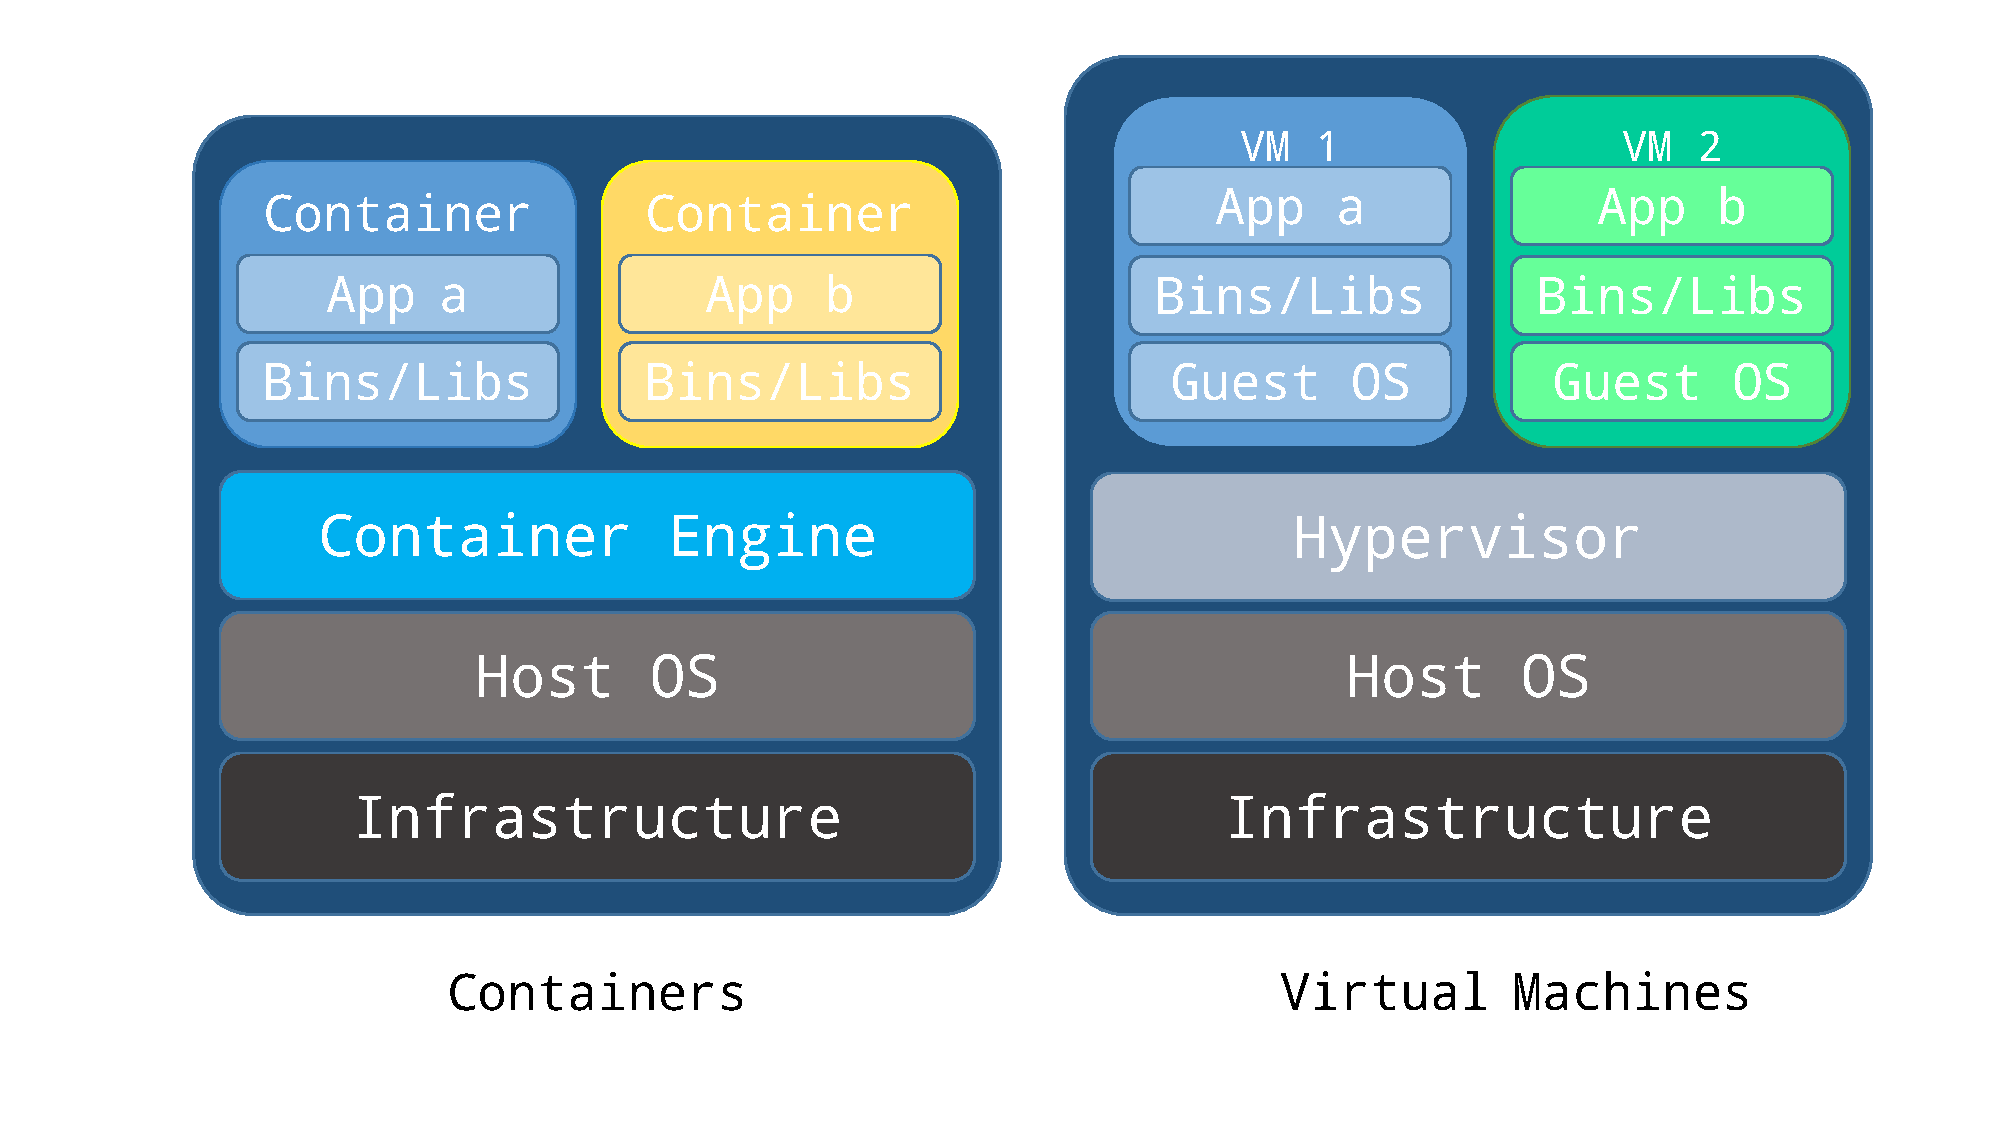
\includegraphics[width=0.9\textwidth]{./figure/container-vm}
\bicaption[fig:container_vs_vm]{容器和虚拟机架构对比}{\textbf{容器虚拟化} VS \textbf{虚拟机}}{Fig}{Containerization VS Virtual Machine}
\end{figure}

图\ref{fig:container_vs_vm}显示了容器虚拟化技术和虚拟机之间技术框架的差异:不同于虚拟机,容器实例之间共享主机操作系统和相同的依赖库,各实例只需要单独处理各自不同的依赖库安装和环境设置。

\section{负载预测}
针对历史数据的分析和预测有很多方法,从简单的平均算法、回归算法到复杂的人工智能算法。在负载预测领域,整体上可以分为基于时间序列数据\cite{hamilton1994time}分析的预测模型和非时间序列数据的预测模型。

基于时间序列数据的预测已经被广泛研究和应用在计量金融学、天气预报和地震预报等领域。时序数据的分析预测模型有很多,其中经典的模型有:
\begin{enumerate}
\item 自回归滑动平均(autoregressive moving average, ARMA)模型和差分整合移动平均自回归(autoregressive integrated moving average, ARIMA)模型,这两个模型都是基于移动平均(Moving Average, MA)模型和逻辑回归(Autoregressive, AR)模型\cite{box2015time}。这类模型受限于本身自相关系数的影响,预测结果通常相比观测值有一定的滞后性,Yang等也发现相比ARIMA模型和ARMA模型,一元线性回归模型有更高的预测精确度\cite{yang2013workload};
\item 基于移动平均模型的扩展还有指数移动平均(Exponential Moving Average,EMA)模型\cite{xiao2013dynamic}和加权移动平均(Weighted Moving Average,WMA)\cite{wu1989time},Huang等发现双重指数平滑模型因为能够反映出变化趋势,因此比起单纯的平均模型和加权平均模型由更高的预测精度\cite{huang2012resource};
\item 自回归条件异方差模型(Autoregressive conditional heteroskedasticity,ARCH)模型\cite{bollerslev1986generalized}则在应对波动形的时间序列数据场景下有出色的表现,在金融领域中被广泛应用于风险预测。Adegboyega则提出在线性模型下,ACS(Adaptive Conditional Score Models)模型相比ARCH模型和ARIMA模型有更高的预测准确率\cite{adegboyega2015dynamic};
\item 基于隐式马尔科夫模型的卡尔曼滤波(Kalman Filtering)模型\cite{goodwin2014adaptive}在短期预测中有较好的表现,但是由于该模型只是根据上一时刻的数据进行分析预测,因此并不适合周期性变化特征的场景下。Mark等发现,相比于基于简单卡尔曼滤波的预测模型,基于二次指数平滑的预测模型能提供更高的预测准确率和更少的预测开销\cite{mark2011evolutionary};
\item 成长曲线(Growth Curve)模型中成长速度随着时间增长而增长,Višnja Križanović等发现Gompertz曲线模型的预测曲线可以很好地跟随观测曲线的增长\cite{vcik2016comparison}。Lu等提出一个优化的预测模型,负载增加时使用Gompertz曲线模型进行预测,而在负载下降时使用移动平均模型来预测,提供了一定的预测准确率\cite{lu2014dynamic}。
\end{enumerate}

非时序数据的预测主要表现为基于人工智能技术的预测模型,常见的模型有人工神经网络(Artificial Neural Network)模型、支持向量机(Support Vector Machine,SVM)模型和高斯过程(Gaussian Process)模型等。除了上述模型之外,Jheng等还提出了一种基于灰度系统的负载预测模型\cite{jheng2014novel}。他们通过在灰度系统中根据时间的相关性来对未来的负载进行预测。获取前四周周一的相同时间的历史记录,然后利用灰度模型可以得到接下来的周一同一时间上的负载预测值。该模型在负载增加时预测值和实际值比较相近,但是在负载下降时预测值始终高于实际值。这些人工智能模型的有点在于相比时间序列在应对周期性负载模式时预测精度较高,同时因为采用的是离线学习模式,可以对历史数据进行大量的分析。这是基于时间序列数据的预测难以做到的,但是也因为离线学习的问题,导致不能应对突发的负载变化。

Kim等选择了21个负载预测模型并对这些负载预测模型进行了评估\cite{kim2016empirical}。他们将负载的预测模型分成四个种类:简单预测模型、基于回归的预测模型、基于时间序列数据分析的预测模型和非时间序列数据的负载预测模型。其中,简单预测模型是对数据取平均值或者取最近K个数据求平均值的预测模型。根据最终的评测结果,SVM模型具有最高的预测精确度,WMA模型和ARMA模型的精确度紧随其后,简单预测模型的预测精度最差。但是SVM模型作为离线学习模型,只适用于周期性变化的场景,不能将实时的负载变化加入到之后的预测分析中,ARMA模型在历史数据较多的场景下预测分析的速度最慢,难以应对突发的变化。WMA模型和多层神经网络模型的耗时最少,但是多层神经网络模型在21个预测模型中只有中等的预测精度。

Pati等提出将多层前向神经网络模型和ARIMA模型相结合,能获得相比单独的神经网络模型和单独的ARIMA模型更高的预测精度\cite{pati2014comparison}。他们将负载模型分为线性模型部分和非线性模型部分,通过ARIMA模型来得出线性模型的预测值,多层前向神经网络来得到非线性模型的预测值,然后将两者结合得到最终的预测结果。他们针对的预测对象是Debian系统的漏洞数,预测的时效性在面对随着时间迅速变化的负载场景并不适用。

以上提及的预测模型都有着各自的优点和缺点,整体而言,基于时间序列数据分析的预测模型适用于短期变化的场景,而基于机器学习的预测模型则适用于长期的预测。但是由于现实中复杂的负载变化场景,没有任何一个通用的预测模型能满足现实中的负载预测。我们只能针对不同的负载变化场景,根据负载数据进行分析和预测。

\section{资源供给}
云计算中提出的“pay-as-you-go”模型理论上根据用户的实际需要动态分配资源,收费时则根据用户使用的实际资源总量进行计价\cite{armbrust2010view}。然而目前在实际使用中,云服务提供商都需要用户自己指定需要的资源数目,而不是用户实际的SLA\cite{patel2009service}。这导致用户常常为了确保自身的正常使用而申请过多的资源从而造成资源浪费,或者预计的资源并不足以应对实际的负载导致不能到达一开始的服务目标。为了应对上述的问题,Chaisiri等提出一个基于确定性等价式的资源供给优化算法,提供一个满足基本需要的长期资源供给方案和一个能根据负载现状立刻调整的短期资源供给方案,其中长期方案资源消耗更少,短期方案消耗更多\cite{chaisiri2012optimization}。他们的资源优化算法针对的是由用户选择云服务提供商提供资源供给方案的场景,没有从云服务提供商层面出发,使得资源供给方案不够灵活,仍然会造成较多的资源浪费。

Le等基于排队论理论,认为可以根据任务队列中任务的平均等候时间来动态的调整资源使用量\cite{le2013dynamic}。根据任务队列中当前和上一个任务之间的出队时间差当作任务的运行时间,基于M/M/1队列模型根据虚拟机的CPU计算能力计算任务队列中每个任务所需要的虚拟机数量,从而决定对虚拟机资源池进行伸缩。这个方案整体目标是让所有任务可以在用户设定的截止时间之前完成,只考虑了CPU的消耗,没有考虑存储和网络带宽等其他因素,同时资源调整的粒度仍然是虚拟机粒度,没有考虑资源伸缩需要的开销和资源的浪费。

Wu等通过将SLA映射到云服务的服务质量(Quality of Service,QoS),得到一个基于SLA的资源供给模型\cite{wu2014sla}。该模型基于最适配原则提出了两个优化的资源供给算法。这两个算法相比单纯的查找最优适配算法,减少了虚拟机迁移的开销,总体上提高了用户SLA的满足率。第一个算法的优化对比算法中针对找不到相同类型请求的合适虚拟机实例是通过新建虚拟机实例来实现的,因此实际中的优化优先。第二个算法的问题则是需要通过大量的冗余来规避虚拟机迁移造成的额外开销,随着请求种类的增加冗余也会大量增加,使云服务提供商产生额外的成本。

针对数据迁移需要跨物理机房的场景,Chase等提出一个基于随机规划模型的资源供给方案\cite{chase2017joint}。他们将虚拟机迁移所需要的带宽作为资源供给算法计算的一部分,利用场景树缩减算法来尽可能快的提供一个合理的启发式结果。但是该模型没有考虑虚拟机迁移过程中网络传输的耗时,同时由于现实网络环境的异构性,导致对该问题的分析极其复杂。

Guo等针对空间上分离的云服务提供商,提出一个基于排队论中G/G/1模型的主动式资源供给方案\cite{guo2016geoscale}。通过检测不同地区的云服务中任务的等待时间和平均服务时间从而得出每个云服务中需要的虚拟机数目,然后根据虚拟机数目对各云服务中的实例进行伸缩,利用各个云服务的本地行来降低不同云服务之间的迁移开销。然而这个方案直接对虚拟机进行水平伸缩,没有考虑使用垂直伸缩来降低迁移操作本身的开销。

\section{负载应对}
负载均衡作为在多计算资源间分配负载,实现最优化资源使用和提高吞吐量等目标的技术,在国内外已经有广泛的研究。Randles等对三种分布式负载均衡方案进行了比较和讨论\cite{randles2010comparative}。该论文探讨的三种分布式负载均衡算法在伸缩性上有较好的表现,但是没有考虑系统伸缩过程中对吞吐量造成的影响和开销。

Hu等提出一个基于遗传算法的负载均衡分配方案\cite{hu2010scheduling}。通过遗传算法得到当前环境下最优的负载分布,然后根据最优的负载分布找到从当前状态调整过去开销最少的策略则是满足目标的负载均衡方案。然而该方案假定所有的虚拟机服务能力始终一致,没有考虑服务器垂直伸缩的问题。同时基于遗传算法,最后得出的解可能只是局部最优解而不是全局最优解。

Alizadeh等针对数据中心网络流量巨大的现状,设计并实现了一个基于网络层拥塞感知的分布式负载均衡模型\cite{alizadeh2014conga}。由于数据中心的特性,采用中心化的负载均衡方案将导致负载均衡模块难以应对巨大的流量请求,从而成为性能瓶颈。这篇论文从传统的基于网络流量的角度设计了一个分布式的负载均衡器,但是没有考虑到数据中心内实际运行的服务器本身的处理能力,可能出现虽然某些服务器带宽资源充足但是其他诸如CPU能力或者内存等资源不充足的场景,这样单纯按照带宽进行分配反而会造成资源分配不合理,导致性能的下降和资源的浪费。

Wang等参照负载均衡中负载窃取算法,提出一个面向数据敏感的基于自适应负载窃取算法的负载均衡模型\cite{wang2014optimizing}。该论文建立了一个去中心化的负载均衡模型,提供了更高的健壮性和可伸缩性,但是主要针对的是数据敏感的场景,并不具有普适性。该模型研究的场景下所有的虚拟机都是相同的服务能力,也没有考虑不同虚拟机之间实际服务能力不同的问题。

以上论文大多设计了分布式的负载均衡方案,提升了可伸缩性和健壮性,但是也基本都是只以带宽资源作为负载均衡的调节基准,没有考虑到实际中各服务实例的服务能力的差异。随着过去几年云计算的急速发展,通过更好的调度任务和分配资源来应对负载变化的方案也在被广泛研究。Li等研究了虚拟机在集群中的成本最小化放置方法,并提出了一个权衡了网络流量和物理设备成本的最优化算法\cite{li2014let}。Peng等构建了一个基于文件块的虚拟机镜像分发网络,从而加速了虚拟机实例的部署和启动速度\cite{peng2012vdn}。Harter等构建了基于中央式存储服务的存储驱动Slacker,加速了容器在集群中部署和启动,但是这需要额外的网络文件系统(NFS)存储服务器提供基于文件系统层面的专门支持\cite{harter2016slacker}。Gog等基于最小费用最大流(MCMF)算法提出了中央式调度器Firmament来降低放置过程的延迟\cite{gog2016firmament}。Kaewkasi等基于蚁群算法提出一个新的启发式算法来确定Docker swarm集群中任务和资源的分配和管理,从而提升了集群整体的性能\cite{kaewkasi2017improvement}。然而,以上方案都忽视了资源和任务的调整对可用性的影响。

\section{本章小结}
对于云服务提供商而言,如何做到在保证满足SLA的同时尽可能提高资源使用率,减少资源浪费从而降低整体成本仍然是一个重要的问题。将这个问题拆分成两个子问题,则分别是满足SLA和提高资源使用率。基于预测的方案可以提前采取伸缩控制资源供给应对负载的变化,避免由于负载变化来不及调整导致违反SLA;而为了提高资源使用率,可以引入负载均衡的策略。但是目前相应的方案仍然存在很多问题:首先,现有的云资源供给方案大多基于虚拟机这一虚拟化技术,相比轻量级的容器虚拟化技术而言,虚拟机间的资源迁移操作本身耗时更长,额外的资源开销更多;其次,已有的负载均衡方案大多是从网络流量本身的角度考虑的,没有考虑虚拟机除带宽资源以外能提供的服务能力;然后,已有的负载应对方案没有考虑容量调整操作本身耗时带来的影响,使得整体的调整总是落后于负载的变化了;最后,针对容器集群的解决方案都忽视了用户对可用性的约束。本课题为了解决上述问题,提出一个基于容器的主动式云负载均衡模型。和传统的根据负载实时状态进行集群伸缩的响应式调整策略不同,该模型试图通过对负载进行监测后预测将来一段时间的负载,然后根据预测的负载提前对容器云进行伸缩,在保证服务本身可用性的前提下,减少应对负载变化所需要的延迟,提升容器云整体的性能。
%# -*- coding: utf-8-unix -*-
%%==================================================
%% chapter01.tex for SJTU Master Thesis
%%==================================================

\algnewcommand\algorithmicforeach{\textbf{for each}}
\algdef{S}[FOR]{ForEach}[1]{\algorithmicforeach\ #1\ \algorithmicdo}
%\bibliographystyle{sjtu2}%[此处用于每章都生产参考文献]
\chapter{系统设计}\label{chap:sys_design}
\section{容器云相关技术分析}
\subsection{Docker镜像}
Docker镜像是Docker容器运行的基础,提供了运行容器所需要的依赖环境和环境配置。Docker镜像本身基于分层文件系统,将所有的文件变化和环境配置变更都作为内部文件系统层级的变更,本质上是一个包含着一系列文件系统层级修改的有序集合\footnote{https://docs.docker.com/glossary/?term=image}。由于Docker容器利用了写入时复制(copy-on-write,CoW)作为容器内部分层式文件系统读写策略,基于同一Docker镜像创建的不同容器实例可以共享这个镜像底层的文件系统,这也大大方便了Docker镜像的制作。因此,Docker用户常常会引用其他基础镜像作为自身镜像的基础。

\begin{table}[h]
\centering
\bicaption[tb:dist_size]{不同Linux发行版本镜像在最受欢迎应用镜像中引用的分布情况}{不同Linux发行版本镜像在最受欢迎应用镜像中引用的分布情况}{Table}{Linux Distribution Images References In Most Popular 30 Application Images on Docker Hub}
\begin{tabular}{@{}llrr@{}}\toprule
 发行版本 & 版本代号 & Docker镜像大小(MB) & 引用计数 \\ \midrule
 Debian & Jessie & 123 & 25\\
 Ubuntu & Xenial & 119 & 3\\
 Alpine & 3.6 & 5 & 2\\ \bottomrule
\end{tabular}
\end{table}

除此之外,Docker在1.10版本之后引入了内容寻址功能,使得Docker镜像中的同一文件层级在不同机器和实例中都有相同的唯一标识,大大方便了Docker容器在不同环境下的迁移\footnote{https://github.com/moby/moby/wiki/Engine-v1.10.0-content-addressability-migration}。这个新的特性使得即使是基于不同Docker镜像构建的容器也能共享底层的部分共用镜像,比如相同的操作系统镜像和运行时环境等。为了调查不同镜像在底层基础镜像上的共享情况,我们在目前最受欢迎的容器镜像仓库,同时也是官方镜像仓库Docker Hub\footnote{https://hub.docker.com/}上对当前最流行的30个应用镜像进行调查,得到的统计结果如表\ref{tb:dist_size}所示。由表\ref{tb:dist_size}可知,大量的应用镜像依赖于少数几种底层基础镜像。考虑到对网络流量和存储空间的影响,这些基础镜像的大小是很重要的。尽管用户可以选择基于\emph{Alpine}或者\emph{scratch}这类更小的镜像来制作容器镜像,但是由于诸如\emph{Debian} 或者\emph{Ubuntu}等Linux发行版本通常默认自带诸如\emph{apt}和\emph{wget}等有用的工具而且环境设置更友好,大家还是更喜欢使用这些自己更熟悉的Linux发行版本来管理依赖环境和环境配置。

\subsection{已有的容器集群管理框架}
\begin{figure}[htbp]
\centering
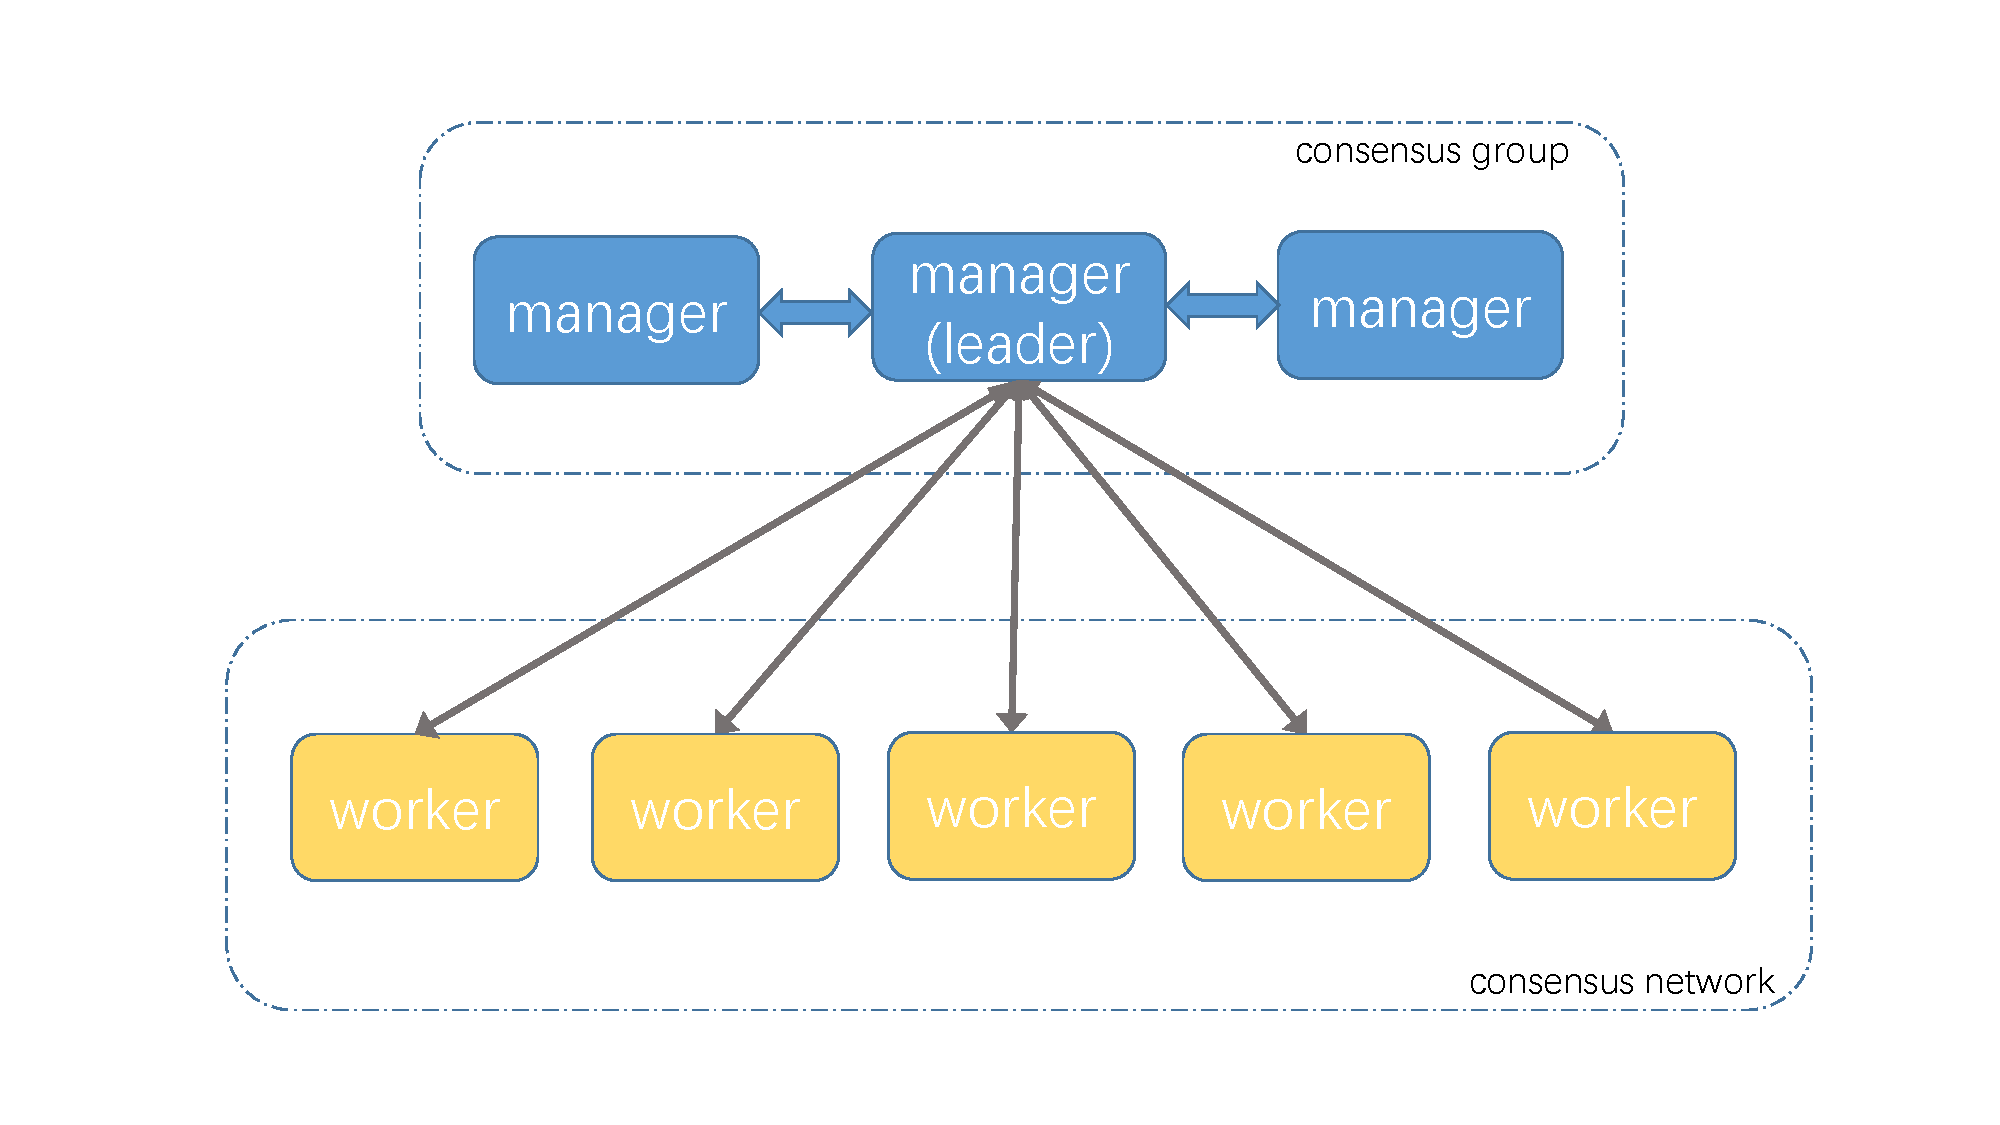
\includegraphics[width=0.9\textwidth]{./figure/manager-worker}
\bicaption[fig:manager-worker]{集群的分布式系统架构}{\textbf{集群的分布式系统架构}}{Fig}{Architecture in Container Cluster}
\end{figure}
当前主流的容器集群管理框架都是基于分布式系统架构进行设计,将每个物理服务器作为集群中的节点来构建分布式的集群。如图\ref{fig:manager-worker}所示,在当前主流的容器集群框架设计中,集群中的节点分为两类:管理者节点和工作者节点。管理者节点之间通过诸如paxos和raft等一致性协议构建一致性群组,从而实现容器集群中管理者功能的高可用;工作者节点基于gossip等一致性协议构建一致性网络,保证数据在工作者节点之间的一致性;管理者节点按照所选择的一致性协议周期性地从所有管理者节点中选择出领导者节点,领导者节点和工作者节点之间进行通信并将数据同步给其他的管理者节点。

目前构建容器云常用的框架主要有Docker Swarm、Kubernetes和Mesos,其中Docker在1.12版本之后引入了swarmkit作为原生的swarm mode提供了默认的Docker容器集群支持,这三者针对负载变化的场景均只能通过修改副本数的方式来进行容量调整。在独立的Docker Swarm中,提供三个不同的调度策略供用户选择:\emph{spread}模式,\emph{binpack}模式和\emph{random}模式。其中,\emph{spread}模式将任务平均分配到集群中所有的节点上;\emph{binpack}模式则恰恰相反,使用贪心算法将任务分配到当前可以选择的任务最多的节点上,优先将集群中的节点按照装箱的方式依次装满;\emph{binpack}模式则先筛选符合条件的集群节点,然后将任务随机的分配到其中的一个节点上。在Docker swarm mode中,目前只支持和\emph{spread}模式分配思路一样的\emph{SpreadOver}模式。Kubernetes则通过插件的方式提供多种调度模式的支持,包括但不限于按节点资源使用量均分、按节点任务数均分、资源利用率最高的节点优先和资源利用率最低的节点优先等,其中也支持将使用相同镜像的容器聚集的模式,但是要求必须是同一个容器镜像。Mesos则作为一个分布式资源框架,要求用户自己实现调度器或者使用诸如Marathon\footnote{https://mesosphere.github.io/marathon}等第三方调度框架,默认不提供任何负载均衡和资源调度的支持。综上而言,目前已有的各个容器调度框架没有针对可用性和负载变化进行区分,没有默认的服务可用性支持,需要用户手动控制副本数以满足服务的可用性,通过变更服务的副本数来应对负载的变化;各框架更多的关注于提升整体资源利用率,而忽视了服务可用性和服务容量变化成本之间的平衡。

\section{系统架构}
本课题以资源使用率作为实际负载的衡量标准,提出基于容器的主动式容器云负载优化模型,旨在在负载多变的场景下,加速容器云中服务对负载变化的响应,加强容器云对负载变化的灵活性,从而更好的应对负载,提升容器云整体的服务质量。模型的整体架构设计如图\ref{fig:sys_design}所示,一共分为资源使用状态监测、资源使用状态预测、资源供给方案生成、资源供给优化、资源管理和负载均衡等6 个模块。由于应用于容器云这一分布式的架构环境中,本课题提出的模型中各模块也将基于分布式架构的思想来设计,以提升整体模型的性能和可靠性。
\begin{figure}[htbp]
\centering
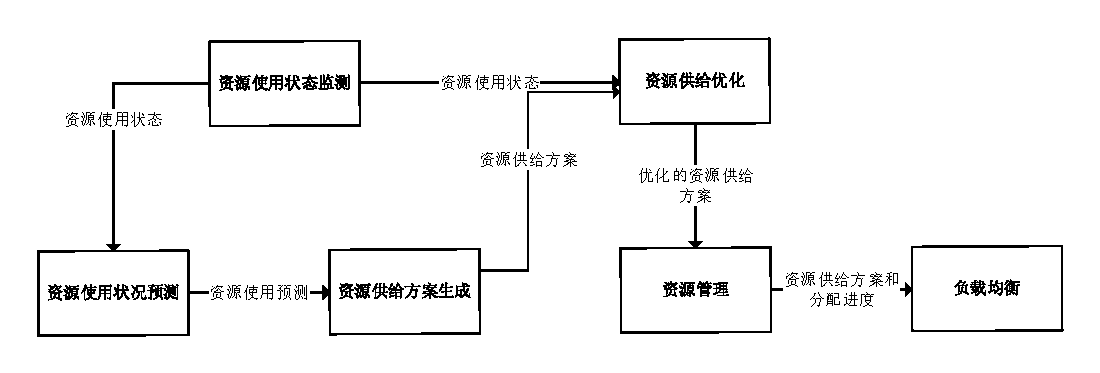
\includegraphics[width=0.9\textwidth]{./figure/sys_design}
\bicaption[fig:sys_design]{系统架构设计}{\textbf{系统架构设计}}{Fig}{System Architecture}
\end{figure}

我们将整个模型框架分为三个部分:负载监测和预测、资源供给和管理以及负载应对。其中,负载监测和预测部分包括了架构设计中的资源使用状态监测模块和资源使用状态预测模块;资源供给和管理部分包含了资源供给方案生成模块、资源供给优化模块和资源管理模块;负载应对部分则包括了负载优化模块。其中,资源供给和管理部分主要负责对本系统内服务资源的使用状态进行监测并给予历史监测数据给出未来一段时间内的资源使用预测;资源供给和管理部分基于可用性分析,根据预测的资源使用量和实际的监测状态得到需要的任务实例数目;负载应对部分则依据当前容器云中所有节点的状态和目标服务的限制通过服务伸缩的操作选择合适的节点来托管相应任务实例,从而达到更好的应对负载变化的目标。由于本模型应用于容器云中,所以本质上是一个分布式框架,很多模块利用消息队列通过周期性的异步操作来提升整体的吞吐量,提高框架的整体性能。本文接下来将分别对这三部分进行说明从而介绍整个架构中各模块的设计和涉及的核心技术及算法。

\section{负载监测和预测}
\subsection{资源使用状态监测模块}\label{sec:monitor}
资源使用状态常常随着负载的变化而变化,当负载上升时,相应资源的使用量会相应的增加;当负载下降时,对应资源的使用量则会相对的减少。通过对负载的实时监测,我们可以及时把握负载的状态,并根据负载的变化对服务进行相应的调整,保证服务质量的同时降低成本。同时,对负载的实时记录可以作为原始数据,通过预测等方法进一步的提升服务质量,降低成本。在本课题中,我们用系统中资源的使用状态来表征当时的负载状态,对资源的使用状态进行周期性的监控,并将观测到的结果按照时序数据的格式记录下来。在容器云中,可使用资源的种类可分为以下4 种:CPU、内存、磁盘存储和网络带宽。但是考虑到在目前的主流容器云和管理框架中,主要使用诸如AWS的Amazon Simple Storage Service(S3)等云存储服务,很少使用对应节点上的物理硬盘,我们在本课题中监测的资源类型包括:CPU使用状态、内存使用状态和网络带宽使用状态。容器云本身是一个分布式架构,因此我们通过在容器云中各节点上对各节点本身以及运行在节点上各个任务实例的资源使用状态进行监测,并通过心跳包的传输方式周期性地向容器云中的管理者节点同步各任务实例的资源使用状态和作为集群节点的物理服务器的资源使用状态。为了后续方便后续预测的处理,我们使用时间序列数据的格式来保存监控到的资源使用状态,具体的数据格式如公式\ref{eq:res_format}所示:
\begin{equation}\label{eq:res_format}
\{time, (cu, ca, mu, ma, niu, nia, nou, noa)\}
\end{equation}

在公式\ref{eq:res_format}中,$time$表示该次监测操作的时间点,按Unix时间戳的格式记录,即该时间点到1970年1月1日0点正的毫秒数;$cu$表示此次监测观测到的已使用CPU个数,$ca$表示被监控对象可用的CPU个数,单位均为一个标准CPU核;$mu$表示本次监测观测到的内存使用大小,$ma$代表被监控对象可用的内存大小,单位均为字节(即Byte);$niu$表示本次监测中观测到的网络接收速度,$nia$表示被监控对象的最大可用网络接收速度,$nou$表示本次监测中观测到的网络发送速度,$noa$表示被监控对象的最大可用网络发送速度,单位均为bps。由于网络的发送/接受速度无法通过已有的接口直接获取,必须基于计算两次监控间隔之间发送/接受网络包数量的差值进行计算,计算方法如公式\ref{eq:net_speed}所示:
\begin{equation}\label{eq:net_speed}
networkSpeed_t = \frac{packageSize_t-packageSize_{t-1}}{time_t-time_{t-1}}
\end{equation}
其中,$packageSize_t$表示此次监控观测$t$时刻的网络数据包大小,$packageSize_{t-1}$表示上一次监控${t-1}$时刻观测的网络数据包大小,$time_t-time_{t-1}$表示这两个监控时刻之间的时间差。

资源使用状态监测模块默认每隔100ms对资源使用状态进行一次采集,并且每隔30秒将该时段内的监控数据从各个工作者节点同步管理者节点。每次采集时,除了资源使用状态的信息之外,资源使用状态监测模块还会根据监测对象的类型追加其他的标记数据:如果监测的是集群节点,则标记该数据为节点类型并在资源使用状态数据后追加集群节点的ID;如果监测的是任务实例,则标记该数据为任务实例类型并在资源使用状态数据后追加任务实例的ID和相应服务的ID。在同步之前,资源使用状态监测模块会对采集到的原始监控数据进行预处理,通过对每个时间段内的数据取均值后作为这段时间内的观测数据,以减小短时间内观测值的波动,降低整体的观测误差和传输的数据大小,这个时间段默认为3秒。通过标准化所有监控数据的时间记录点,使得所有节点上报的监控数据中采样时间点一致,从而可以获得集群中所有节点和服务在相应时刻的状态。

\subsection{资源使用状态预测模块}\label{sec:prediction}
目前的框架和容器云均是在资源使用量达到指定阈值后按照诸如实例数翻倍等特定规则进行的自动伸缩。但是在不同的负载场景下使用相同的规则会出现很多问题。以实例翻倍的伸缩策略为例,在负载急剧增加的场景下,按照实例翻倍的策略进行一次调节后仍然不能满足负载的需要,必须通过多次调节才能满足负载的变化。但这就造成了相应延迟,并降低了这一阶段内的服务质量。而在负载增长缓慢的场景下,实例数量翻倍后虽然满足了负载的需要,但是多分配了额外的资源,增加了成本。因此通过可靠的方法对将来的负载状态进行预测,从而可以获知应对相应负载所需要的资源,能更好地保证容器云中的服务质量,降低整体的成本。在本课题提出的模型中,资源使用状态预测模块周期性的对之后一段时间内的资源使用量进行预测。资源使用状态监测模块获得历史监测数据后会将相应数据周期性地给资源使用状态预测模块,默认周期为5分钟。由于资源使用状态监测模块能够提供的最新数据是来自前一个周期的资源使用状态数据,而预测操作本身需要耗费时间,因此在资源使用状态预测模块中对当前周期进行预测显然会造成相应的延迟。为此资源使用状态预测模块根据当前所属周期t之前获得的历史监测数据,利用相应的预测算法对再下一个周期t+1内的资源使用量进行预测。即在默认情况下,资源使用状态预测模块会通过预测算法预测从5分钟之后开始到10分钟之后这个5分钟时间段内服务所需要的资源使用状态,预测结果的数据格式如公式\ref{eq:pred_format}所示:
\begin{equation}\label{eq:pred_format}
\{time, (cu, mu, niu, nou)\}
\end{equation}
其中中,$time$表示下一个周期开始的时间,按Unix时间戳的格式记录,即该时间点到1970年1月1日0点正的毫秒数;$cu$表示预测要使用的CPU个数,单位均为一个标准CPU核;$mu$表示本次预测得到的内存使用大小,单位均为字节(即Byte);$niu$和$nou$分别表示预测要使用的网络接收速度和网络发送速度,单位均为bps。

目前主流的预测方法主要分为基于经典时间序列理论的预测方法和基于人工智能的预测方法两大种类,两类算法各有优缺点:基于经典时间序列理论的预测方法速度更快,但是更多表现为预测结果相对于实际结果的延迟,预测精度较低并且预测值准确度和周期参数设置紧密相关,更加适用于有明显周期性的数据;基于人工智能的预测算法需要额外的数据训练过程,但是由于除了时间特征之外可以加入业务相关特征,因此预测准确性更高。我们引入了预测正确率等预测模型评估标准来帮助我们评估预测模型在容器云环境下的预测准确性和预测结果对后续调整的影响。我们在资源使用状态预测模块中引入了经典时间序列理论的预测算法模块和基于人工智能的预测算法模块供用户选择使用,分别选择基于整合移动平均自回归模型的预测算法和基于长短期记忆模型\cite{hochreiter1997long}的预测算法作为基于经典时间序列理论的预测算法默认实现和基于人工智能的预测算法默认实现。

最后,我们使用开源的98年世界杯网站流量数据\cite{arlitt2000workload}作为用户请求的模拟数据,并且假定每次请求消耗相同的资源和CPU时间。在接下来的几节中,我们将分别对预测模型评估标准进行介绍,并对使用基于整合移动平均自回归平均模型预测算法和基于长短期记忆模型预测算法作为默认预测算法实现的原因进行分析和讨论。

\subsubsection{预测模型评估标准}
在实际中,预测结果往往并不是十分准确,但是我们可以通过在依赖预测结果的基础上根据实际状态进行再次调整的方式来提高系统整体的灵活性,从而进一步地提升系统对负载变化的应对能力。如果预测结果比实际需要的资源总量低,那就导致基于预测分配的资源不足以应付实际的负载,降低整体的服务质量;如果预测结果高于实际需要的资源总量,虽然存在资源的浪费但保证了服务的稳定可用,保障了服务的质量。除此之外,根据Google对Borg的使用分析,在容器云中创建容器的延迟远远比预期的更加严重\cite{verma2015large}。因此,为了更好地响应负载变化,我们自然希望尽量是通过收缩的方式来实现对服务实例规模的调整。为了客观评估预测算法对实际调整的影响,我们在评估容器云中的预测算法效果时引入了预测正确率这一概念,预测正确率计算方法如公式\ref{eq:correctness}:
\begin{equation}\label{eq:correctness}
Correctness_{algo} = \frac{Count(Usage_{predication} >= Usage_{actual})}{Count(Usage_{actual})}
\end{equation}
从公式\ref{eq:correctness}中可以很明显地发现,预测算法可以通过增加自身预测值的方法来提升自身的预测正确率。在保证尽量在预测的结果进行收缩的方式来调整服务实例规模的基础上,我们依然希望相应预测算法能尽量减少预测偏差,从而尽可能的减少资源的浪费。我们引入了预测偏差率$\overline{ME}$和预测偏方差率$\overline{MSE}$来量化地表示预测结果和实际观测值之间的差距,预测偏差率$\overline{ME}$可以量化地表征预测算法的准确性,而预测偏方差率$\overline{MSE}$则可以用量化的方式来表征预测算法预测结果的稳定性,详细计算方法分别如公式\ref{eq:algo_error}和公式\ref{eq:algo_mse}所示:
\begin{equation}\label{eq:algo_error}
\overline{ME_{algo}} = \frac{\sum_{time \in period} {\frac{\vert Usage_{predication_{time}} - Usage_{actual_{time}}\vert}{Usage_{actual_{time}}}}}{Count(time)}
\end{equation}
\begin{equation}\label{eq:algo_mse}
\overline{MSE_{algo}} = \frac{\sum_{time \in period} {\frac{\vert Usage_{predication_{time}}^{2} - Usage_{actual_{time}}^{2}\vert}{Usage_{actual_{time}}^{2}}}}{Count(time)}
\end{equation}

\subsubsection{基于整合移动平均自回归模型的预测算法}
整合移动平均自回归(ARIMA)模型作为经典时间序列预测理论的代表模型,通过对一段时间内的历史数据进行分析从而计算出接下来周期内的预测值。对于有明显周期性质的时间序列数据而言,整合移动平均自回归模型的预测过程更加直观并且准确率较高,在诸如如金融证券市场等具有明显周期性的应用场景中被广泛应用。整合移动平均自回归模型可以看作是一个包含了自回归模型和滑动平均模型的结合,通过差分的方式对时序数据平稳化,利用自回归模型的特性来记录历史值对当前的影响,通过滑动平均模型来描述累积的误差影响。

\subsubsection{基于长短期记忆模型的预测算法}
时间递归神经网络(RNN,Recurrent Nerual Networks)模型通过引入循环的方式使得神经网络中的信息可以持久化\cite{graves2012supervised},因此时间递归神经网络模型很适合应用于时序数据这一具有明显时间依赖的场景中。相比于基于经典时间序列理论的预测算法,基于时间递归神经网络模型的模型除了时间序列本身的特征外还能引入其他业务特性来标记时间序列本身的状态,从而加强模型的表征能力,提高预测精度。但是传统的时间递归神经网络模型很难解决长期依赖的问题:要训练过程中的计算量随着记忆的历史数据增加呈指数型增长\cite{bengio1994learning}。长短期记忆(LSTM,Long Short-Term Memory)模型作为一种时间递归神经网络模型的变种,通过独特的门结构来解决传统时间递归神经网络模型中长期依赖导致问题。对于本文提出的模型而言,由于资源使用状态的监控周期很短,导致得到的时间序列数据规模必然很大,因此使用长短期记忆模型更有助于分析此类数据。

\section{资源供给和管理}
在容器云中,负载的监控和预测仅仅是第一步,我们仍然需要根据预测的结果和实时的监控信息来控制和管理各个服务的资源使用,确保每个服务有足够的资源可以应对自身的负载,并且尽量减少资源的浪费。除此之外,我们还需要需要根据各个服务的可用性目标确认满足该目标所需要的副本数,以及收集各个节点上其他诸如层级文件缓存状态信息等工作。在本课题提出的模型中,这些任务都由资源供给和管理部分负责处理。资源供给和管理部分分为资源供给方案生成模块、资源供给优化模块和资源管理模块三个模块:
\begin{enumerate}
\item 资源供给方案生成模块负责周期性地根据资源使用状态预测模块中的预测结果生成下一时间段的资源分配方案,确定满足相应资源需求所需要的实例数;
\item 当实际监控的资源使用状态和预测不相符时,资源供给优化模块负责根据实时的监控状态对当前的服务实例规模进行优化调整;
\item 资源管理模块负责根据确认的服务实例规模向负载优化模块发起服务伸缩请求,基于本模型中的服务可用性模型确认服务所需的副本数。除此之外,资源管理模块还负责收集集群中各节点上的层级文件缓存信息和利用Docker \emph{Registry} API获取运行服务所需Docker镜像的元信息。
\end{enumerate}
我们将在接下来的几个小节中对服务可用性模型和以上三个模块进行详细介绍。

\subsection{资源供给方案生成模块}\label{sec:provision_active}
资源使用状态预测模块根据资源使用状态的历史记录预测出了下一个周期的资源使用量,但是仅仅只有资源使用量并不能完成容器云中服务的伸缩操作,我们需要依据相应的资源使用量计算得到所需要的实例数。同时,由于预测不可能百分之百的准确,我们对预测的使用量追加了额外的资源份额,即默认预测资源使用量为实际资源请求的95\%。在资源供给方案生成模块中,我们根据得到的各项资源使用量预测值和服务运行单个实例所需要的各类资源,计算出满足预测的资源使用量所需要的服务实例数目,详细过程如算法\ref{algo:instance_for_resource}所示:
\begin{algorithm}[h]
\caption{满足资源使用量的实例数}
\label{algo:instance_for_resource}
\begin{algorithmic}[0]
\\
\Require ~~\
\\
$resources$: resource usage for the service;\\
$taskReq$: resource requirement for tasks of the service;\\
$elasticPer$: the percentage for elasticity
\Ensure ~~\
\\
size of instances \\

\Function {instancesofresources}{$resources$, $taskReq$}
    \ForEach{ resource type}
        \State $resource_{type} \gets  \lceil \frac{resource_{type}}{{elasticPer} \times {taskReq_{type}}} \rceil$
    \EndFor
    \State \Return $\max_{\forall type \in resources} {(resource_{type})}$;
\EndFunction
\end{algorithmic}
\end{algorithm}

资源供给方案生成模块周期性地从资源使用状态预测模块获得下一个周期的资源使用量预测并确认相关服务所需要的资源供给方案。资源供给方案生成模块默认以5分钟作为一个周期,从资源使用状态预测模块获得对下一个周期的资源使用量预测。算法\ref{algo:instance_in_period}显示了资源供给方案生成模块确认下一个周内所需任务实例数的具体过程:
\begin{algorithm}[H]
\caption{计算下一个周期的实例数}
\label{algo:instance_in_period}
\begin{algorithmic}[0]
\\
\Require ~~\
\\
$resourcesSeries$: resource usages in future period;\\
$taskReq$: task specification for the service;
\Ensure ~~\
\\
the size of service instances in the following period\\

\ForEach{$resources$, $time$ in $resourcesSeries$}
    \State $instances_{time} \gets \Call{instancesofresources}{{resources}, {taskReq}}$
\EndFor
\State \Return $\max_{\forall time \in resourcesSeries} {(instances_{time})}$
\end{algorithmic}
\end{algorithm}

从算法\ref{algo:instance_in_period}中我们可以发现,输入的参数中是一个包含了多个监控时间段的资源使用量预测的数组,而相应的输出结果却是一个实例规模大小而不是相应的实例数量的数组。这是因为服务伸缩操作本身也是一个需要一定时间开销的耗时操作,短时间内频繁的伸缩调整会导致系统整体性能出现抖动。为了兼顾系统整体的稳定性和服务伸缩的及时性,资源供给方案生成模块对一个周期内的资源使用量只进行一次服务规模调整,即在该周期开始时进行一次伸缩并保证在此次调整之后服务的实例规模能应对这个周期内所有的负载变化。

资源供给方案生成模块得到下一个周期的实例数后按照公式\ref{eq:instances_format}的格式将相应的预测实例数发送给资源管理模块:
\begin{equation}\label{eq:instances_format}
\{time, instance\}
\end{equation}
其中,$time$表示此次实例调整开始的时间,按Unix时间戳的格式记录,即该时间点到1970年1月1日0点正的毫秒数;$instance$表示本次预测最终需要的实例数。随后,资源管理模块会根据接收到的实例预测结果,根据其中预测的规模变化时间和相应的实例规模大小对相应服务的实例规模进行调整。

\subsection{资源供给优化模块}\label{sec:provision_react}
虽然我们利用资源使用状态预测模块得到了下一个周期资源使用量的预测结果,但是由于预测结果并不能保证百分之百的准确,很多时候预测结果仍然只能用作趋势的预测分析,而不能用作最终的确认结果。特别是当负载的增加速度超过预测时,为了能保证实际的服务质量不会由于激增的负载而降低,我们必须快速响应负载的变化,因此需要根据实际监测到的的资源使用量立刻重新调整服务的实例规模。我们根据资源供给方案生成模块中设定的额外资源比例,在资源供给优化模块中设定95\%作为资源使用状态的默认扩展警戒阈值。除此之外,现实中的负载必然会出现瞬时的突发变化,比如某个时刻负载突然增加或者突然降低,然后负载状态又回归正常趋势。对于这种小概率的突发情况,如果处理这种异常情况那必然会导致服务在极短时间内规模的来回伸缩,这明显会影响服务本身的稳定性,同时也会增大服务整体的运行维护成本。因此,我们需要在每个时间周期内对这种异常情况进行统计,只有当指定时间周期内负载变化超过预期阈值若干次后再对服务的实例规模进行调整,从而避免为了应对短时间内为数不多的几次负载变化而对服务进行伸缩反而导致整体的服务质量出现抖动。资源供给优化模块通过启发式算法分别对资源使用量持续超过阈值和持续低于阈值的场景进行分析,并得到相应时间段内服务实际需要的实例规模大小。

当资源使用量在指定时间周期内持续超过扩展警戒阈值,资源供给优化模块通过一个启发式的算法\ref{algo:instance_increasing},根据从资源使用状态监测模块周期性的获取资源使用状态监控数据,并判断如果在连续2个周期内任意一个周期长度的时间内实际资源使用状态超过扩展警戒阈值5次即需要对服务实例规模进行优化调整,默认处理方式是将当前任务实例规模大小增加5\%。
\begin{algorithm}[H]
\caption{资源使用量超过扩展警戒阈值}
\label{algo:instance_increasing}
\begin{algorithmic}[0]
\\
\Require ~~\
\\
$resourcesSeries$: resource usage in the last two periods;\\
$instanceScale$: size of service instances at the moment;\\
$warningLevel$: the warning level for actual resources usage \\
$scaleTrigger$: the number of resouce usages counts the warning level \\
$scalePercentage$: the scaleup percentage for the service
\Ensure ~~\
\\
size of instances for the service \\

\ForEach{ $resources, time \in resourcesSeries$}
    \ForEach{ resource type}
        \If{$resourceUsage_{type} > resourceAllocated_{type} \times {warningLevel}$}
            \ForEach{ $previous \in increasing$}
                \If{$previous$ and $time$ not in a period}
                    \State $increasing.remove(previous)$
                \Else
                    \State break
                \EndIf
            \EndFor
            \State $increasing.add(time)$
        \EndIf
        \If{$size(increasing) > scaleTrigger$}
            \State \Return $instanceScale \times (1+scalePercentage)$
        \EndIf
    \EndFor
    \State \Return $instanceScale$
\EndFor
\end{algorithmic}
\end{algorithm}

当实际的资源使用量在指定时间周期内持续少于收缩警戒阈值时,资源供给优化模块通过减少服务的实例数来提高资源利用率,降低整体的成本。资源供给优化模块设定50\%作为资源使用状态的默认收缩警戒阈值,并同样通过一个启发式的算法计算合适的实例规模大小。通过从资源使用状态监测模块周期性的获取资源使用状态监控数据,并判断如果在连续2个周期内实际资源使用状态不低于于收缩警戒阈值少于5次即需要对服务实例规模进行优化调整,默认为将当前任务实例规模减少为原来50\%,具体过程如算法\ref{algo:instance_decreasing}所示:
\begin{algorithm}[H]
\caption{资源使用量远低于收缩警戒阈值}
\label{algo:instance_decreasing}
\begin{algorithmic}[0]
\\
\Require ~~\
\\
$resourcesSeries$: resource usage in the last two periods;\\
$instanceScale$: size of service instances at the moment;\\
$warningLevel$: the warning level for actual resources usage \\
$scaleTrigger$: the number of resouce usages counts the warning level \\
$scalePercentage$: the scaleup percentage for the service
\Ensure ~~\
\\
size of instances for the service \\

\ForEach{ $resources, time \in resourcesSeries$}
    \ForEach{ resource type}
        \If{$resourceUsage_{type} \geqslant resourceAllocated_{type} \times {warningLevel}$}
            \State $decreasing.add(time)$
            \State break;
        \EndIf
    \EndFor
    \If{$size(decreasing) < scaleTrigger$}
        \State \Return $instanceScale \times (1-scalePercentage)$
    \Else
        \State \Return $instanceScale$
    \EndIf
\EndFor
\end{algorithmic}
\end{algorithm}

相比于负载增加而言,负载减少对整体服务质量和性能的影响较小,主要影响体现在成本控制方面。本文优先考虑满足服务的可用性目标和保证服务质量,因此在负载迅速降低的场景下只对和预测差异比较大的情况(即长时间低于收缩警戒值)做应急处理,其他情况则由资源管理模块根据预测的资源使用量进行调整。
当资源供给优化模块根据负载状态确认最终需要的实例规模之后,将数据按照公式\ref{eq:instances_format}的格式发送给资源管理模块进行实际的服务伸缩调整。

\subsection{服务可用性模型}\label{sec:availability_model}
不同于目前其他的容器集群框架,本课题提出的服务可用性模型将容器云中每个运行着相关任务实例的托管节点作为服务的一个副本,而不是将服务的每个任务实例作为该服务的一个副本。在本课题提出的模型中,每个至少运行着一个该服务任务实例的托管节点被当作该服务的一个副本。本课题将容器云中每个托管节点的可用性,即该节点设备正常工作的概率,作为为该服务在这个节点上的可用性指标。因此,在本课题提出的模型中,容器云中服务的可用性可以根据该服务相关任务实例在整个集群中托管节点的分布进行计算得到。集群中每个节点的可用性可按照公式\ref{eq:valid}进行计算:
\begin{equation}\label{eq:valid}
\begin{split}
availability = \frac{MTBF}{MTBF + MTTR}
\end{split}
\end{equation}
其中MTBF(Mean Time Between Failures)表示该节点的平均故障间隔,MTTR(Mean Time To Recovery)表示该节点的平均恢复时间。根据节点的可用性, 我们可以利用公式\ref{eq:avail}计算出集群中服务\emph{s}的可用性$P_{available_s}$:
\begin{equation}\label{eq:avail}
\begin{split}
P_{available\_s} = 1 - \prod_{i \in {replica(s)}} \overline P_{i},
\end{split}
\end{equation}
在公式\ref{eq:avail}中$P_{i}$表示容器托管节点$node_i$作为服务\emph{s}副本的可用性,并且基于此我们可以算出$\overline P_{i}$ = 1 - $P_{i}$。公式\ref{eq:avail}中等式右侧第二项表示整个服务的所有副本在容器云中均失效导致服务整体失效从而无法继续提供服务的概率。根据该可用性模型,我们可以发现在本课题提出的模型中,服务通过副本节点在容器云中的分布状态来满足自己的可用性目标从而保证服务的可用性。这也就意味这我们可以依据容器云中相关服务副本的实时分布状态计算出该服务当时的可用性指标。

对一个由具有相同可用性指标的节点构成的同构容器集群而言,容器云中服务的可用性仅仅和该服务实际的副本数目相关,服务\emph{s}对副本数目的要求即为满足其可用性目标所需要的最少副本数。假设容器云中每个容器托管节点的可用性指标为$P_{valid}$,服务\emph{s}的可用性目标为$P_{available_s}$,由于容器云中每个节点失效无法工作的概率是相同的,因此我们可以根据公式\ref{eq:replica}反向推导,从而计算出服务\emph{s}需要的副本数:
\begin{equation}\label{eq:replica}
\begin{split}
replica_s = \lceil \log_{1-P_{valid}} ( 1 - P_{available\_s} )\rceil.
\end{split}
\end{equation}

\subsection{资源管理模块}\label{sec:provision_utils}
资源供给方案生成模块和资源供给优化模块分别给出了基于预测的资源使用量和实际的资源使用量得到的服务实例数,并发送给资源管理模块。资源管理模块内部维护一个时间间隔为10秒的定时器,周期性检查这段时间内收到的基于预测的服务实例调整请求,当到达相应时间后向负载优化模块发起服务伸缩请求,由负载优化模块处理具体的服务伸缩操作。对于由资源供给优化模块发出的实时调节请求,资源管理模块立刻根据请求的实例数向负载优化模块发起服务伸缩请求。在节点可用性同构的容器云中创建服务时,资源管理模块会基于公式\ref{eq:replica}算出该服务所需要的副本数,而无需用户指定副本数;在其他类型的容器云中,用户可以手动指定服务需要的副本规模。在发起服务伸缩请求之前,资源管理模块会对请求的实例数和需要的副本数进行比较,基于算法\ref{algo:instance_with_replica}确认最终的任务实例数,确保最终发送的服务伸缩请求中实例数不少于副本数。
\begin{algorithm}[H]
\caption{基于副本数确认实例规模}
\label{algo:instance_with_replica}
\begin{algorithmic}[0]
\\
\Require ~~\
\\
$instance$: proposed instance number;\\
$replica$: number of replicas for the service;
\Ensure ~~\
\\
valid instance number\\

\State \Return $\max {(instance, replica)}$;
\end{algorithmic}
\end{algorithm}

除此之外,资源管理模块还负责同步容器云中各节点上的层级文件缓存信息和利用Docker \emph{Registry} API获取服务运行所需要的Docker镜像中的元数据信息。为了获取容器云中节点上层级文件的缓存信息,我们需要在Docker \emph{Engine}中新增一个接口,周期性地将各个节点上的层级文件缓存信息增量式地同步到管理者节点,为后续服务伸缩调度决策提供计算基础。

\section{负载应对}
在容器云中,我们通过对服务进行伸缩的方式来应对负载的变化。由于在本课题的模型中,服务的可用性指标可以由服务的副本数来表征,因此我们在服务创建时除了需要指定实例数,还需要指定该服务需要的副本数以满足可用性要求;在服务伸缩时,则是通过改变实例数的方式来保证在不违反原先设定的副本要求前提下,利用负载优化模块对任务实例的调度选择进行优化,从而实现更好地应对负载变化的目标。

\subsection{负载优化模块}\label{sec:scheduler}
在实际生活中,负载更多时间处于非平稳无周期的状态,这种场景下当前的预测模型不能进行准确有效的预测。即使是在有平稳周期的负载场景下,我们固然通过预测的方法可以提前获得一个对未来负载状态的估计,但是由于预测本身并不能保证百分百的准确,当预测的负载状态和实际观测到的负载状态不符合时,我们仍然需要根据实际负载做出响应。这就要求我们在确定资源供给方案之后能尽快完成相应任务实例的分发和调度,尽量缩短任务实例在伸缩过程中从准备到实际运行之间的延迟。为此,我们引入了负载优化模块,提升整体对负载变化的响应速度,加强了容器云中服务应对负载的灵活性。负载优化模块根据之前资源供给和管理部分得到的资源供给方案确认了服务所需的任务实例数,基于当前容器云中所有节点的状态和目标服务的限制选择合适的节点来托管相应任务实例,根据服务中任务实例的分布状态和各节点上缓存的Docker镜像层级文件对服务伸缩的操作进行优化,从而达到优化负载应对方案的目标。负载优化模块基于服务需要的任务实例数目和当前实际运行的任务实例数目之间的差异来判断当前服务是否进行伸缩还是保持不变。由于本模块在一个分布式系统中运行,为了提高整体的吞吐量,负载优化模块通过周期性的批处理这一操作方式来应对异步地处理所有的服务伸缩请求。本小节将详细介绍负载优化模块对服务扩展和服务收缩过程的优化。

\subsubsection{服务扩展}\label{sec:scaleout}
当需要的任务实例数目大于当前实际运行的任务实例数时,服务就需要进行扩展以应对负载的增加,保证自身的服务质量。在服务扩展的场景下,负载优化模块将所有新增的任务实例根据服务分类并放入一个等待队列中。在等待队列中,大部分的任务实例都是由于服务扩展的需要而在最近的这个周期内创建的,剩下的小部分则是在之前的周期中创建但是未能成功分配到托管节点或者因为其他原因无法正常启动运行的任务实例。等待队列中任务实例的托管节点选择和分配默认会在5秒之内完成,超时未完成的会被标记为失败后重新进入等待队列准备在下个周期内重新分配。

为了方便对整个过程的说明,我们明确以下几点定义:
\begin{enumerate}
\item 副本数差距(\emph{gap}) 表示相应服务需要的副本数和当前实际的副本数之间的差值。副本数差距如果为正则表示当前的副本数尚不满足服务的副本数要求,还需要\emph{gap}个副本才能达到要求的副本数;否则说明当前服务的副本数已经满足副本要求,没有继续新增副本的必要。
\item 任务节点组代表一个任务实例和一个节点的组合,用来表示一个可能潜在可能的调度安排,即由于这个组合中的节点满足组合中任务实例的各种限制和要求(比如资源要求等),所以这个节点可以运行相应的任务实例。
\item 层级文件一致度表示一个任务节点组合中任务实例运行所需Docker镜像中的层级文件和节点上的层级文件缓存之间的重合度,这由同时出现在任务实例所需Docker镜像和节点层级文件缓存中的层级文件个数确定。
\item 一个任务节点组的优势资源根据组合中任务需要的资源和节点可以提供的资源决定,根据不同资源类型计算任务所需资源和节点可用资源之间的比例,占比最高的则为优势资源。算法\ref{algo:drf}显示了计算一个任务节点组优势资源的过程。
\begin{algorithm}[H]
\caption{计算新增实例的优势资源}
\label{algo:drf}
\begin{algorithmic}[0]
\\
\Require ~~\
\\
$task$: task needed to be scheduled;\\
$node$: nodes in the swarm;
\Ensure ~~\
\\
dominant resource and its proportion\\

\Function {dominantShare}{$task$, $node$}
    \ForEach{ resource type}
    \State $proportion_{type}$ = $\frac{task.reserve_{type}}{node.available_{type}}$
    \EndFor
    \State \Return $\max_{\forall type \in resource} {(proportion_{type})}$;
\EndFunction
\end{algorithmic}
\end{algorithm}
\end{enumerate}

根据我们在第\ref{sec:intro_bg}节中的分析和我们对容器启动过程的分析和测试,依赖环境的下载和安装对容器启动的巨大影响。因此,我们考虑在服务副本实际分布状态满足服务可用性的前提下,尽量利用各个节点上已有的层级文件缓存,从而减少在服务扩展过程中运行新增任务实例的下载耗时和网络开销,降低任务实例启动的延迟,进而加速服务在整个集群中的创建和分发速度,最终实现加快服务扩展过程的目标。为此,本文提出了一个基于启发式多级优先级比较规则的调度选择算法:先将等候队列中的所有新增任务实例和集群中的节点组合成若干个任务节点组,然后依据该启发式优先级比较规则从所有的任务节点组中选择最合适的一组作为一个任务调度选择。该调度选择算法的核心思想是根据启发式的多级优先级比较规则找到优先级最高的任务节点组,算法中用到的多级优先级比较规则如下:
\begin{enumerate}
\item 对于任务节点组中来自不同服务的任务实例而言,相应服务的副本数差距越大则任务节点组的优先级越高;
\item 当任务节点组中任务实例的服务副本数差距相同时,任务节点组的层级文件一致度和优先级正相关,即相应的层级文件一致度越高,任务节点组的优先级越高;
\item 如果任务节点组之间层级文件一致度也一样,那么就比较任务节点组之间的优势资源,优势资源占比越少优先级越高;
\item 采用了以上比较规则后仍然不能确认优先级关系,则根据任务节点组中任务实例和集群节点的\emph{ID}按照字典序比较优先级。
\end{enumerate}

算法\ref{algo:scaleOut}显示了上述启发式调度选择算法的详细过程:
\begin{algorithm}[H]
\caption{服务扩展选择}
\label{algo:scaleOut}
\begin{algorithmic}[0]
\\
\Require ~~\
\\
$tasks$: tasks needed to be scheduled, grouped by corresponding services;\\
$nodes$: nodes in the swarm;
\Ensure ~~\
\\
$scheduling\_decisions$: the task-node pairs in order \\

\While { $tasks$ not empty }
    \ForEach{$task_{i}$ in ${tasks}$}
        \ForEach{$node_{j}$ in ${nodes}$}
            \If{$node_{j}$.meet\_constraints($task_{i}$)}
                \State $pairs$.add($task_{i}$, $node_{j}$);
            \EndIf
        \EndFor
    \EndFor
    \State $suitable$ = ${pair}$ with highest priority in ${pairs}$
    \If{$suitable$ not exists}
        \State break;
    \EndIf
    \State $scheduling\_decisions$.add($suitable$))  
    \State update($tasks$, $nodes$)
\EndWhile
\State \Return $scheduling\_decisions$;
\end{algorithmic}
\end{algorithm}

由算法\ref{algo:scaleOut}可知,等待队列中的所有任务实例按照服务排好序,我们在一个无限循环中对等待队列中的所有任务实例选择合适的托管运行节点,循环直到等待队列为空或者找不到合适的调度选择为止。由于对于同一个服务而言,不同的任务实例之间在限制和资源要求上没有差别,因此在每轮迭代中我们从每个服务中选取一个任务实例作为调度候选者,并从所有候选者中选择一个任务实例作为这轮迭代的最终调度选择。然后我们基于所有的候选者和容器集群中的节点生成相应的任务节点组,并对这些任务节点组基于多级优先级比较规则排序。如果存在优先级最高的任务节点组,那么该任务节点组中的任务实例和集群节点将作为本轮迭代的调度选择。随后更新相应节点的可用资源状态,并将该任务实例从等候队列中移除,同时从该服务中选择下一个等待调度的任务实例作为调度候选者后开始下一轮迭代。由于每轮迭代找到调度选择后被调度节点的可用资源状态都会发生变化,因此我们需要在每轮迭代开始时重新计算所有其他包含该集群节点的任务节点组中的优势资源。如果没有合适的任务调度选择,那么等待队列中剩下的任务实例会被标记为调度失败并等待在下一个调度周期中再次进行调度尝试。

由于负载优化模块的主要目标是在保证服务可用性目标的前提下加速服务的伸缩操作,为此确定调度选择算法中的优先级排序规则十分重要。结合容器云中服务扩展操作的流程,我们基于以下几点考虑设计了服务扩展场景下调度选择算法中使用的优先级比较规则:
\begin{enumerate}
\item 服务的可用性要求是本模型中服务的基本要求,本模型中所有运行的服务必须确保满足自身的副本数要求以保障满足自身的可用性目标。因此服务的副本分布是确定调度选择的基础要素,最终的调度选择必须优先确保每个被调度的服务能够满足自身的副本数要求以保证满足其可用性目标。
\item 层级文件一致度显示了任务实例所需Docker镜像和集群节点在共享层级文件上的契合度,层级文件一致度越高,意味着在该任务实例在相应集群节点上有更多的层级文件缓存可以用,从而减少运行任务实例准备过程中需要下载和安装的层级文件数目和大小,缩短了启动等待时间并减少了集群内部的网络流量。
\item 不同的服务之间对不同的资源需求并不一样,为有着不同资源需求的任务实例寻找合适的托管节点是一个复杂的问题。我们参考了Mesos框架中资源分配的实现,采用了其中\emph{Dominant Resource Fairness(DRF)}算法中的优势资源思想来解决负载优化模块中资源划分的问题,从而实现不同任务间资源分配的帕累托最优\cite{ghodsi2011dominant}。
\end{enumerate}

\subsubsection{服务收缩}\label{sec:scalein}
当服务需要进行收缩时,负载优化模块从当前运行的任务实例中选择合适的停止并关闭。相比服务扩展而言,服务收缩过程中的调度选择更加简单。由于当前运行的服务必然已经在创建和扩展过程中保证满足其自身的可用性需求,我们在服务收缩过程中需要注意的是尽量提高资源利用率并且保证调度不选择不会违反服务的副本数要求。在服务收缩过程中,所有的任务实例已经运行在相应的集群节点上,因此每个任务节点组由相应的任务和托管该实例的节点组成。任务节点组的优势资源计算方法也和服务扩展过程中有所差异,详细计算方法如算法\ref{algo:drf_down}所示:
\begin{algorithm}[H]
\caption{计算已有实例的优势资源}
\label{algo:drf_down}
\begin{algorithmic}[0]
\\
\Require ~~\
\\
$task$: task needed to be scheduled;\\
$node$: nodes in the swarm;
\Ensure ~~\
\\
dominant resource and its proportion\\

\Function {dominantDown}{$task$, $node$}
    \ForEach{ resource type}
        \State $proportion_{type}$ = $\frac{task.reserve_{type}}{task.reserve_{type}+node.available_{type}}$
    \EndFor
    \State \Return $\max_{\forall type \in resource} {(proportion_{type})}$;
\EndFunction
\end{algorithmic}
\end{algorithm}

在服务收缩的场景下,从所有运行的任务实例中确认关闭的任务实例这一调度选择过程和服务扩展场景下的调度选择过程比较相似,都是在确保最终的调度选择不会违背服务副本数要求的前提下,基于启发式的优先级比较规则从所有任务节点组中选择最合适的作为最终的调度选择。但是不同于服务扩展过程中任务实例尚未安置的状态,服务收缩过程是一个资源释放的过程,所有服务的副本分布状态已经满足各自的可用性要求;所有候选任务节点组中的任务实例都已经运行在相应节点上,也不需要考虑不同服务之间的不同类型资源之间的抢占问题;同时服务收缩操作本身相对而言更加迅速,因此在服务收缩的场景下,负载优化模块会立刻发起服务收缩请求而不是如服务扩展过程中通过周期批量操作的方式提高吞吐量。因此,相比于服务扩展场景中的优先级比较规则,服务收缩场景中的优先级比较规则更加简单:
\begin{enumerate}
\item 不同的任务节点组之间,优势资源占比更小则优先级更高;
\item 如果仍然有相同优先级,则根据任务节点组中任务实例和集群节点的\emph{ID}按照字典序比较优先级
\end{enumerate}

算法\ref{algo:scaleIn}显示了服务收缩过程中如何从已运行任务实例中选取合适的任务实例作为最终调度选择:
\begin{algorithm}[!h]
\caption{服务收缩选择}
\label{algo:scaleIn}
\begin{algorithmic}[0] 
\\
\Require ~~\
\\
$down$: the number of tasks needed to be scaled in;\\
$service$: the service to be scaled in;\\
$tasks$: all running tasks of corresponding service;
\Ensure ~~\
\\
$scheduling\_decisions$: tasks to be removed for scale-in \\

\While { down is 0 or no suitable task }
    \ForEach{$task_{i}$ in ${tasks}$}
        \State $node$ = the node that $task_{i}$ current runs on 
        \State $pairs$.add(dominantDown($task_{i}$, $node$));
    \EndFor
    \State $suitable$ = ${pair}$ with highest priority in ${pairs}$
    \State delete($tasks$, $suitable.task$)
    \If{$service$.satisfy\_replica\_requirement($tasks$)}
        \State $scheduling\_decisions$.add($suitable$))
        \State update($nodes$)
    \EndIf
\EndWhile
\State \Return $scheduling\_decisions$;
\end{algorithmic}
\end{algorithm}

在算法\ref{algo:scaleIn}中,我们将相关服务所有在运行的任务实例和相应托管运行的节点作为任务节点组放入一个等待队列中。我们用一个无限循环来从等待队列中挑选合适的任务实例作为最终的调度选择,整个循环直到没有合适的实例可以调度或者已经满足收缩要求停止。由于同一个服务的任务实例可能托管在了同一个集群节点上,因此在每轮迭代开始时,我们需要对等待队列中的人物节点组计算他们的优势资源。在每轮迭代中,根据启发式的优先级比较规则,优先级最高的任务节点组将作为此次迭代可能的调度选择并从等待队列中移除。如果此次调度选择不会违反相关服务的副本数要求,该任务节点组将确认为本轮迭代的最终调度结果并更新相应托管集群节点的可用资源状态;否则,我们会直接抛弃这个可能的调度选择并开始下一轮迭代,在下一轮迭代中从等待队列中剩下的任务节点组里寻找可行的调度选择。我们通过最终的副本数校验操作保证每次的调度选择不会违背服务原定的可用性要求。

\section{本章小结}
本章从系统设计的角度对本文提出的基于容器的主动式容器云负载优化模型进行了详细介绍。我们在本章中将模型的构成分为三个部分:负载监测和预测、资源供给和管理以及负载应对,介绍了各组成部分的结构,并说明了各部分所包含模块之间的联系。随后我们按照不同组成部分的分类,对其中模块的设计和使用到的和核心算法进行了详细的介绍和分析。我们对当前已有的容器云框架进行了深入的探讨和分析,通过引入服务可用性模型和改善当前调度算法的方式对当前容器云框架存在的一些问题提出了解决方案,并对引入的服务可用性模型和任务调度算法进行了分析和讨论。
%# -*- coding: utf-8-unix -*-
%%==================================================
%% chapter01.tex for SJTU Master Thesis
%%==================================================

%\bibliographystyle{sjtu2}%[此处用于每章都生产参考文献]
\chapter{系统实现}\label{chap:sys_impl}
在第\ref{chap:sys_design}章中,我们对本文提出的主动式容器云资源管理模型中各个模块的设计进行了详细的描述。在本章中,我们将根据类图和流程图对这些模块的具体实现进行阐述和讨论。由于本文重点在于对已有容器云中资源管理的优化而不需要关注容器云的构建,因此我们利用Docker \emph{swarm}作为容器云的具体实现,基于Docker 17.04.0-ce版本实现了本文提出的模型。各模块和不同节点之间的数据传输按照基于Protocol Buffers协议进行序列化,并通过gRPC接口进行通信。

由于本文中提出的系统基于Docker实现,对其资源调度模块和服务相关数据类型进行修改并增加了数据监控和预测相关的模块,因此依然沿用了Docker swarm中容器云的整体分发和运行流程。图\ref{fig:swarmkit-modify}显示了以Docker \emph{swarm}框架整体的运行过程:
\begin{figure}[htbp]
\centering
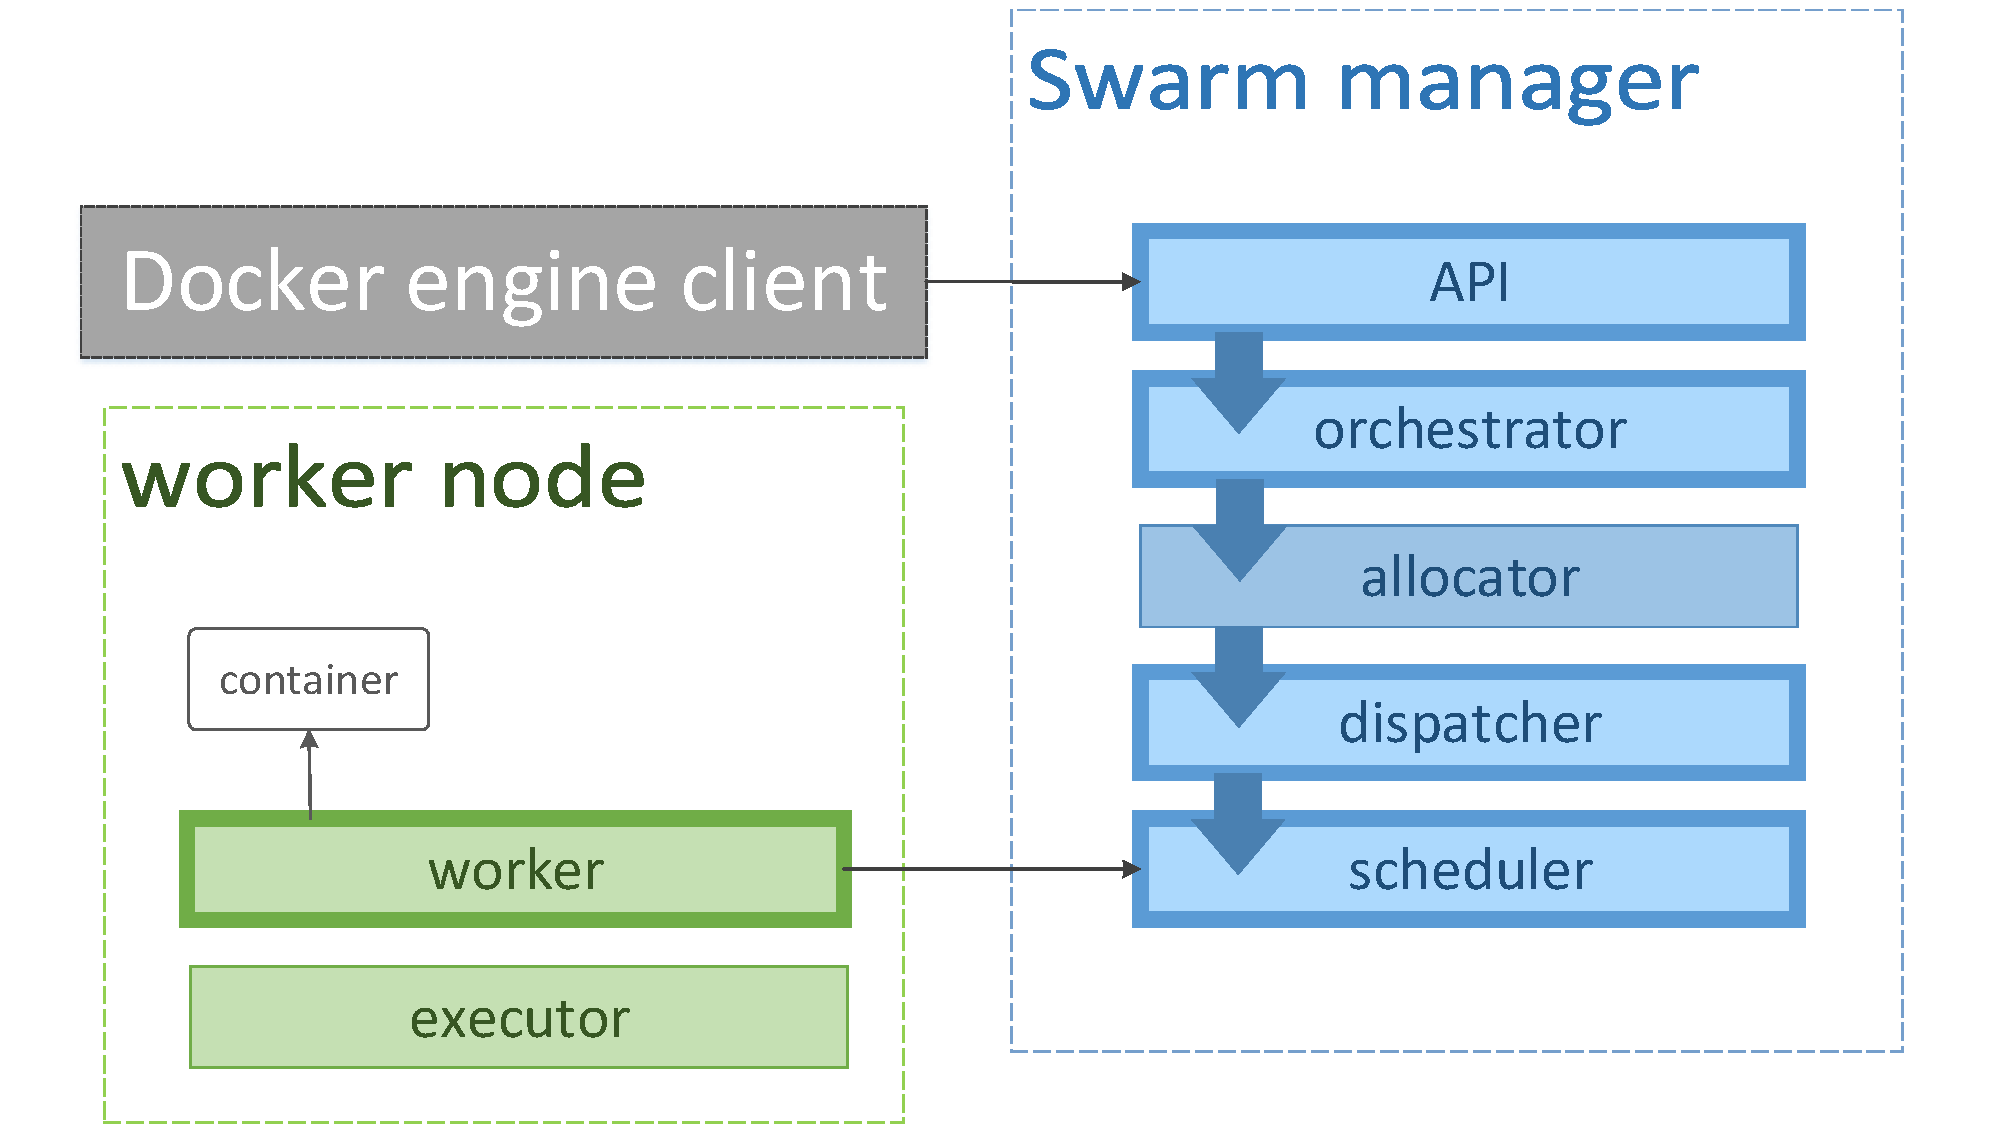
\includegraphics[width=0.9\textwidth]{./figure/modification}
\bicaption[fig:swarmkit-modify]{Docker中服务的运行流程}{\textbf{Docker中服务的运行流程}}{Fig}{How a service works in Docker \emph{swarm}}
\end{figure} 

整体而言,容器云中各个节点分为两种角色:管理者节点和工作者节点,其中管理者节点负责维护容器云中所有节点的信息并根据相应规则将任务的实例分发到相应的工作者节点之中,工作者节点在接受到分配的任务实例利用本节点的Docker Engine来启动容器运行相应的任务实例。对集群的一个节点而言,他必然是一个工作者节点,但是也可以有管理者节点的角色。

\section{资源使用状态监测模块}
图\ref{fig:monitor-impl}显示了资源使用状态监测模块的详细类结构设计:
\begin{figure}[htbp]
\centering
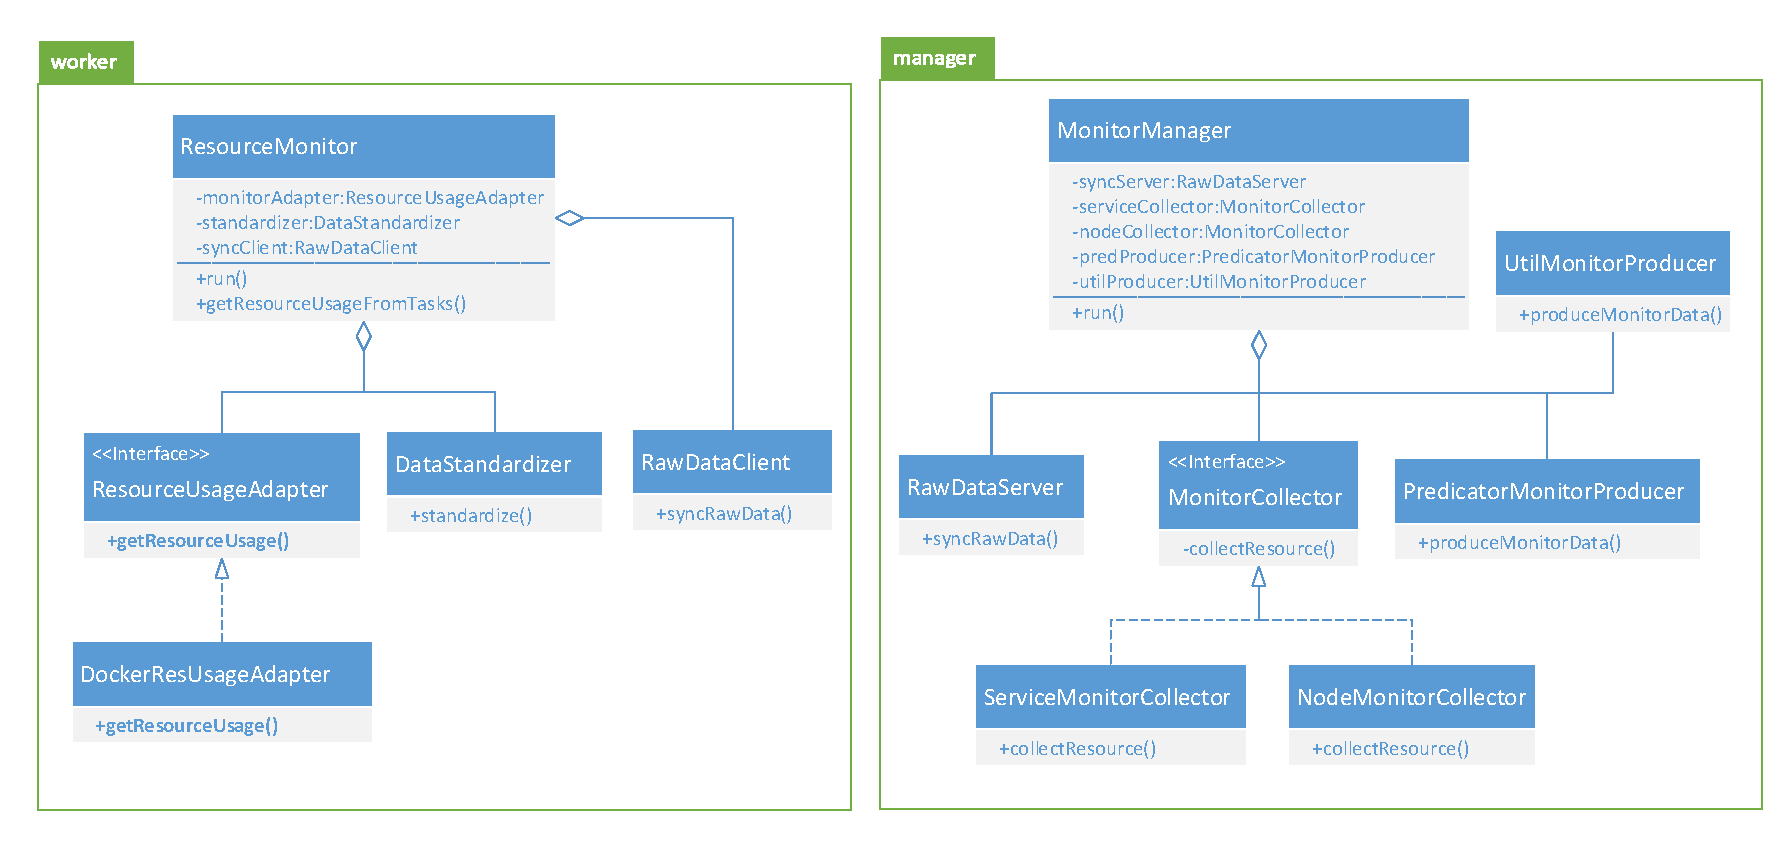
\includegraphics[width=0.9\textwidth]{./figure/monitor_impl}
\bicaption[fig:monitor-impl]{资源使用状态监测模块类图}{\textbf{资源使用状态监测模块类图}}{Fig}{Class Diagram for Resource-Usage Monitor Module}
\end{figure}
由图\ref{fig:monitor-impl}可知,资源使用状态监测模块整体分为manager和worker两个部分,分别运行在容器云中的管理者节点和工作者节点上。在工作者节点上,ResourceMonitor类通过调用getResourceUsageFromTasks方法基于容器中的资源监控接口周期性地获得该节点上所有任务实例的资源使用状态。为了增加可扩展性,方便用户后续加入其它资源属性,我们引入ResourceUsageAdapter接口,通过getResourceUsage方法对资源使用状态进行采集并转换成符合设计部分中提到的数据格式。由于本系统基于Docker实现,我们用DockerResUsageAdapter类来提供ResourceUsageAdapter接口的默认实现类,利用Docker中的状态接口获取各个任务实例和节点本身的资源使用状态,并将相应数据转换成符合本模块需要的格式。类DataStandardizer通过standardize方法对采集到的原始数据进行采样化处理,以3秒为周期对每个周期内的数据取均值后作为这段时间内的观测数据,以减小短时间内观测值的波动,降低整体的观测误差和传输的数据大小。随后,RawDataClient类利用syncRawData方法通过gPRC接口以30秒为周期,将工作节点上统计得到的数据发送给给管理者节点,发送的数据利用Protocol Buffers进行序列化,定义如代码中\ref{code:raw_format}所示:
\begin{lstlisting}[language=protobuf3,style=protobuf, caption={资源使用状态监测数据},label={code:raw_format}]
message ResourceUsageSeries {
    int64 time = 1;
    ResourceUsage usage = 2;
}
message ResourceUsage {
    float cu = 2;
    float ca = 3;
    int64 mu = 4;
    int64 ma = 5;
    int64 niu = 6;
    int64 nia = 7;
    int64 nou = 8;
    int64 noa = 9;
}
message TaskInfo {
    string taskID = 1;
    string serviceID = 2;
}
message RawData {
    ResourceUsageSeries res = 1;
    oneof item {
        string nodeID = 2;
        TaskInfo task = 3;
    }
}
\end{lstlisting}

在管理者节点上,MoniterManager类负责管理整个监控模块的运行周期。RawDataServer类利用syncRawData方法通过gPRC接口从工作者节点的RawDataClient类上接受相应的观测数据。在RawDataServer类获取监控数据之后,MonitorCollector接口通过collectResource方法将相应的资源使用状态监控数据进行整合。ServiceMonitorCollector类和NodeMonitorCollector类作为MonitorCollector接口的具体实现,分别对服务的资源使用状态监控数据和节点的资源使用状态监控数据进行整合。PredicatorMonitorProducer类和UtilMonitorProducer类最后负责利用produceMonitorData方法通过gRPC接口发送给资源使用状态预测模块和资源供给优化模块。

\section{资源使用状态预测模块}
资源使用状态预测模块的类结构设计如图\ref{fig:predicator-impl}所示:
\begin{figure}[H]
\centering
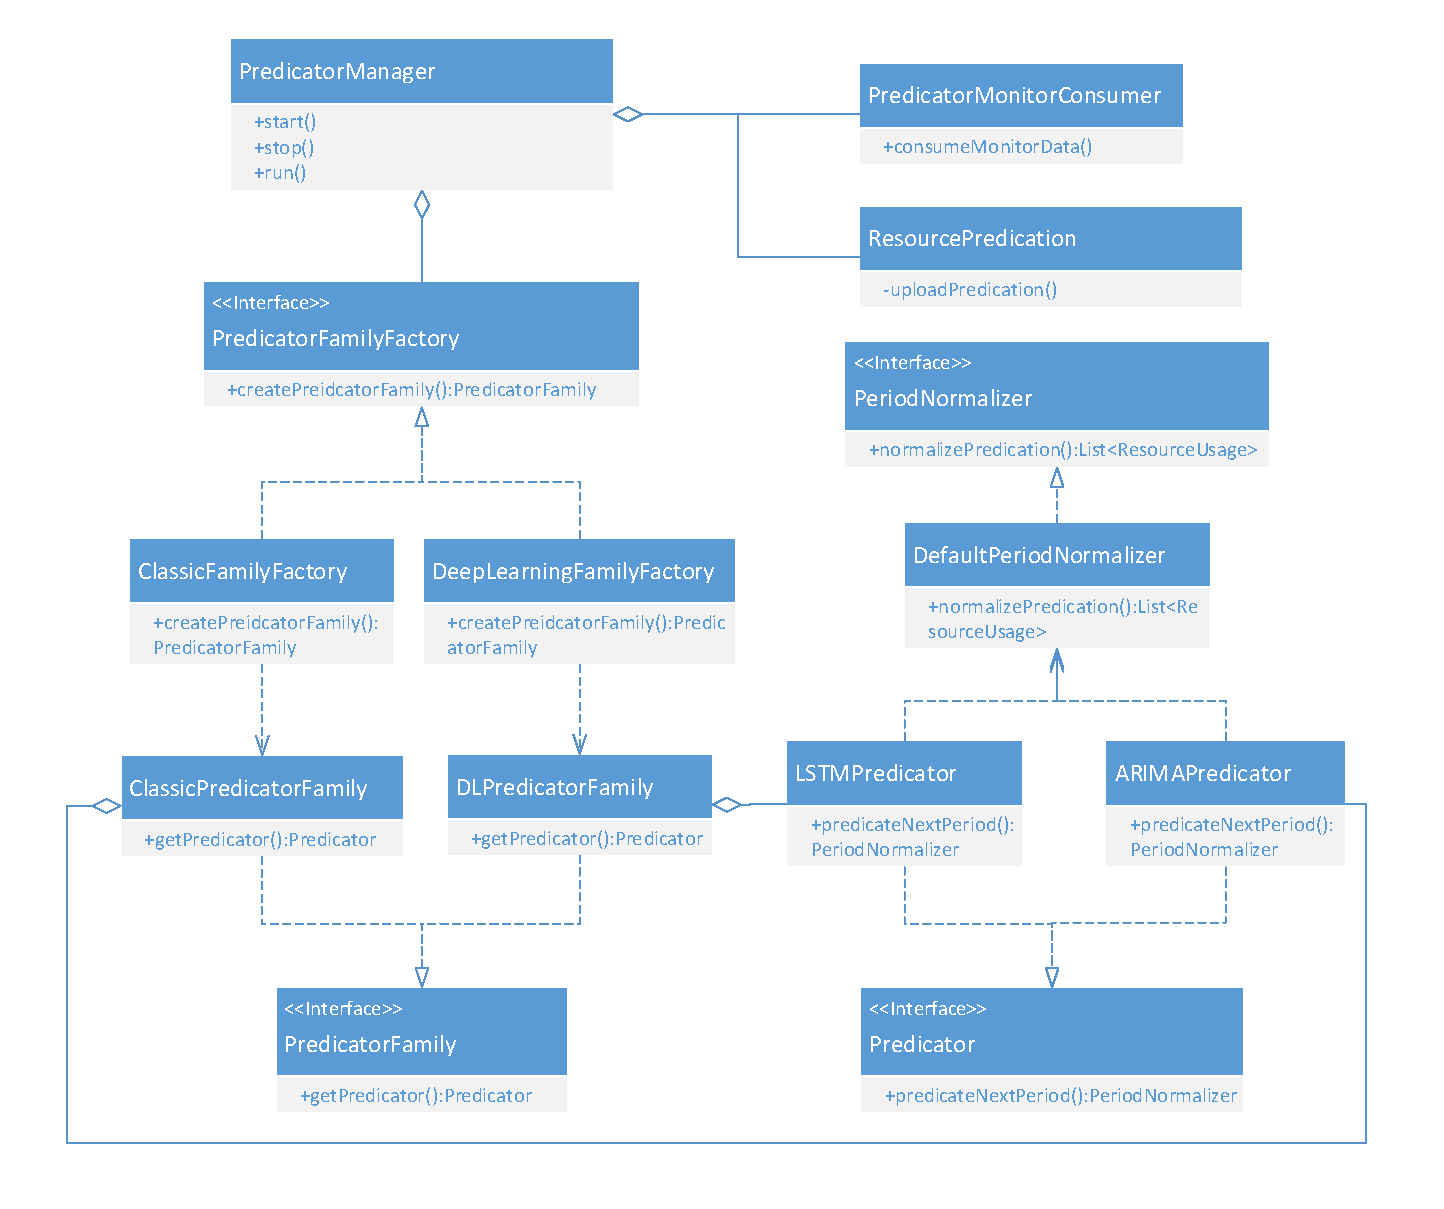
\includegraphics[width=0.9\textwidth]{./figure/predicator_impl}
\bicaption[fig:predicator-impl]{资源使用状态预测模块类图}{\textbf{资源使用状态预测模块类图}}{Fig}{Class Diagram for Resource-Usage Predicator Module}
\end{figure}
PredicatorManager类负责管理整个资源使用状态预测模块的运行周期。我们使用gPRC的方式和资源使用状态监测模块建立RPC通信,PredicatorMonitorConsumer类通过consumeMonitorData方法从资源使用状态监测模块周期性地获取整个容器云中各个服务的资源使用状态数据。资源使用状态预测模块主要负责根据不同的预测算法对历史数据进行预测,但是考虑到实际应用中云环境的复杂性,为了方便用户能够在将来根据自身需要选择其他的预测算法,因此使用抽象工厂的设计模式来实现不同预测处理类的创建,方便后续的扩展。PredicatorFamilyFactory接口中定义了createPreidcatorFamily方法,并通过此方法来生成支持的预测生成器族PredicatorFamily接口。PredicatorFamily接口通过getPredicator方法根据实际需要得到相应的Predicator接口,通过Predicator接口中的predicateNextPeriod方法利用PeriodNormalizer接口获取对下个周期的预测结果,而PeriodNormalizer接口则利用自身的normalizePredication函数来实现获取一个周期内的最终数值调整。最后通过ResourcePredication类中的uploadPredication()方法通过gRPC接口周期性地同步给资源供给方案生成模块。

在本系统中,默认支持基于经典时间序列预测算法和基于深度学习的预测算法,因此PredicatorFamilyFactory接口默认支持两个不同的工厂类型实现:ClassicFamilyFactory类和DeepLearningFamilyFactory类,分别对应基于经典时序数据模型的预测器工厂类型和基于深度学习模型的预测器工厂类型;ClassicPredicatorFamily类和DLPredicatorFamily类分别对应基于经典时序数据模型的预测器族类型和基于深度学习模型的预测器族类型;ARMAPredicator类和LSTMPredicator类分别对应基于ARMA模型的预测器类型和基于LSTM模型的预测器类型;DefaultPeriodNormalizer类为PeriodNormalizer接口的默认实现。在使用基于深度学习模型的预测器来对资源使用状态进行预测之前,用户需要确保已经有经过训练学习的模型可以使用。通过DeepLearningTrainer接口的train方法,用户可以获得根据指定时间范围之内的训练模型,并将此模型用于后续的预测之中。我们使用LSTMTrainer类作为DeepLearningTrainer接口的默认实现,提供基于长短期记忆模型进行预测所需要的模型训练功能。

\section{资源供给方案生成模块}
资源供给方案生成模块的类结构设计如图\ref{fig:provision-impl}所示:
\begin{figure}[H]
\centering
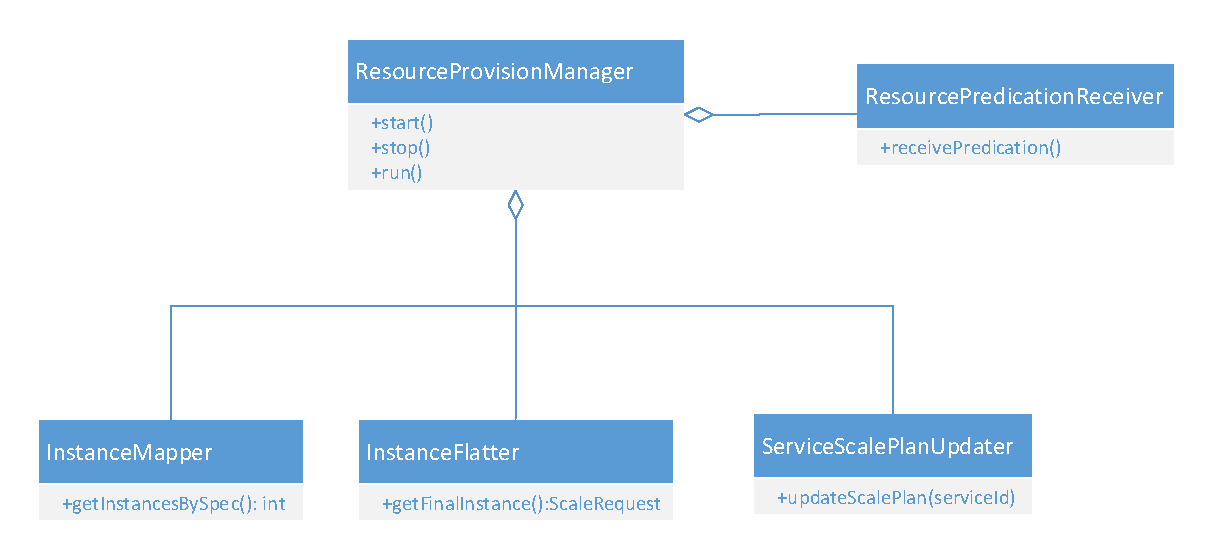
\includegraphics[width=0.9\textwidth]{./figure/provision_impl}
\bicaption[fig:provision-impl]{资源供给方案生成模块类图}{\textbf{资源供给方案生成模块类图}}{Fig}{Class Diagram for Resource Provision Module}
\end{figure}

ResourceProvisionManager类负责管理整个资源供给方案生成模块的运行周期。ResourcePredicationReceiver类利用receivePredication方法从资源使用状态预测模块周期性地接受预测的资源使用量。InstanceMapper类负责根据各个资源的使用量确定需要的任务实例个数,通过getInstancesBySpec方法获得满足资源需求的最少实例数。InstanceFlatter类负责对一个周期内所有的任务实例调整请求进行最终整理和梳理,通过getFinalInstance方法获得本周期内的最终确认的任务实例调整结果。最后,通过ServiceScalePlanUpdater类的updateScalePlan方法将基于预测的实例调整结果通过gRPC接口发送给资源管理模块,数据格式如代码中\ref{code:instance_format}所示:
\begin{lstlisting}[language=protobuf3,style=protobuf, caption={资源使用状态监测数据},label={code:instance_format}]
message ScaleChanges {
    int64 start = 1;
    string serviceID = 2;
    int64 instances = 3;
}
\end{lstlisting}

\section{资源供给优化模块}
资源供给优化模块和资源供给方案生成模块在设计中比较相似,因此具体的实现也和资源供给方案生成模块实现很相近。资源供给优化模块中的类结构设计如图\ref{fig:util-impl}所示:
\begin{figure}[H]
\centering
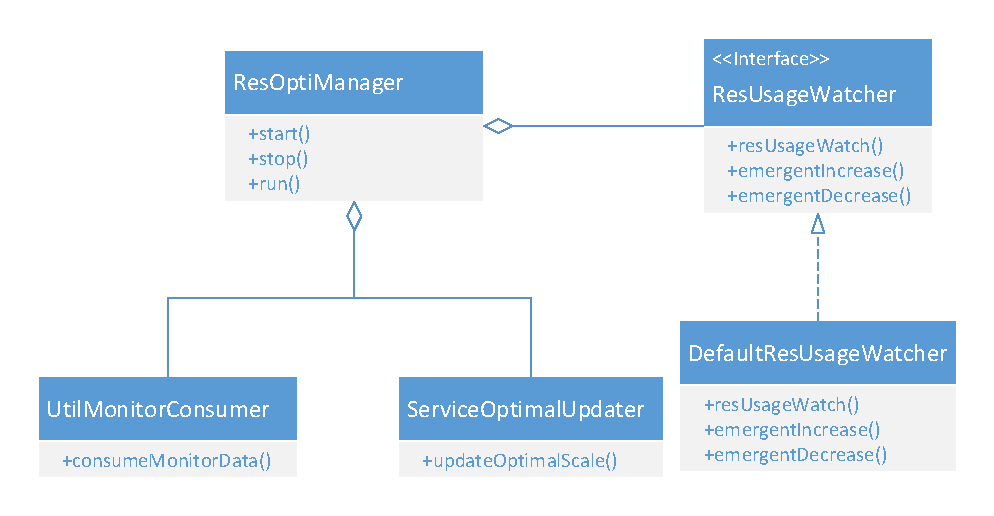
\includegraphics[width=0.9\textwidth]{./figure/optimize_impl}
\bicaption[fig:util-impl]{资源供给优化模块类图}{\textbf{资源供给优化模块类图}}{Fig}{Class Diagram for Resource Optimazation Module}
\end{figure}
ResOptiManager类负责管理整个资源供给优化模块的运行周期。UtilMonitorConsumer类利用心跳的机制,使用consumeMonitorData方法通过gRPC接口从资源使用状态监测模块获取容器云中各个服务和节点的资源使用状态监测数据,ResUsageWatcher接口在resUsageWatch方法中通过检查过去三个周期内的资源使用量是否超过阈值来判断是否需要进行优化调整。当实际资源使用量超过扩展警戒阈值时,ResUsageWatcher接口通过emergentIncrease方法增加实例规模;当实际资源使用量收缩警戒阈值时,ResUsageWatcher接口通过emergentDecrease方法减小实例规模。在本文提出的系统,DefaultResUsageWatcher类是ResUsageWatcher接口的默认实现,使用模块设计中的调整算法。用户可以根据自身的需要,通过实现ResUsageWatcher接口来定制符合自身需要的动态调整方案。如果需要对服务的实例规模进行调整,ServiceOptimalUpdater类通过updateOptimalScale方法将基于计算出的实例调整结果通过gRPC接口发送给资源管理模块,数据格式同样如代码中\ref{code:instance_format}所示。

\section{资源管理模块}
图\ref{fig:manager-impl}显示了资源管理模块中的类结构设计:
\begin{figure}[H]
\centering
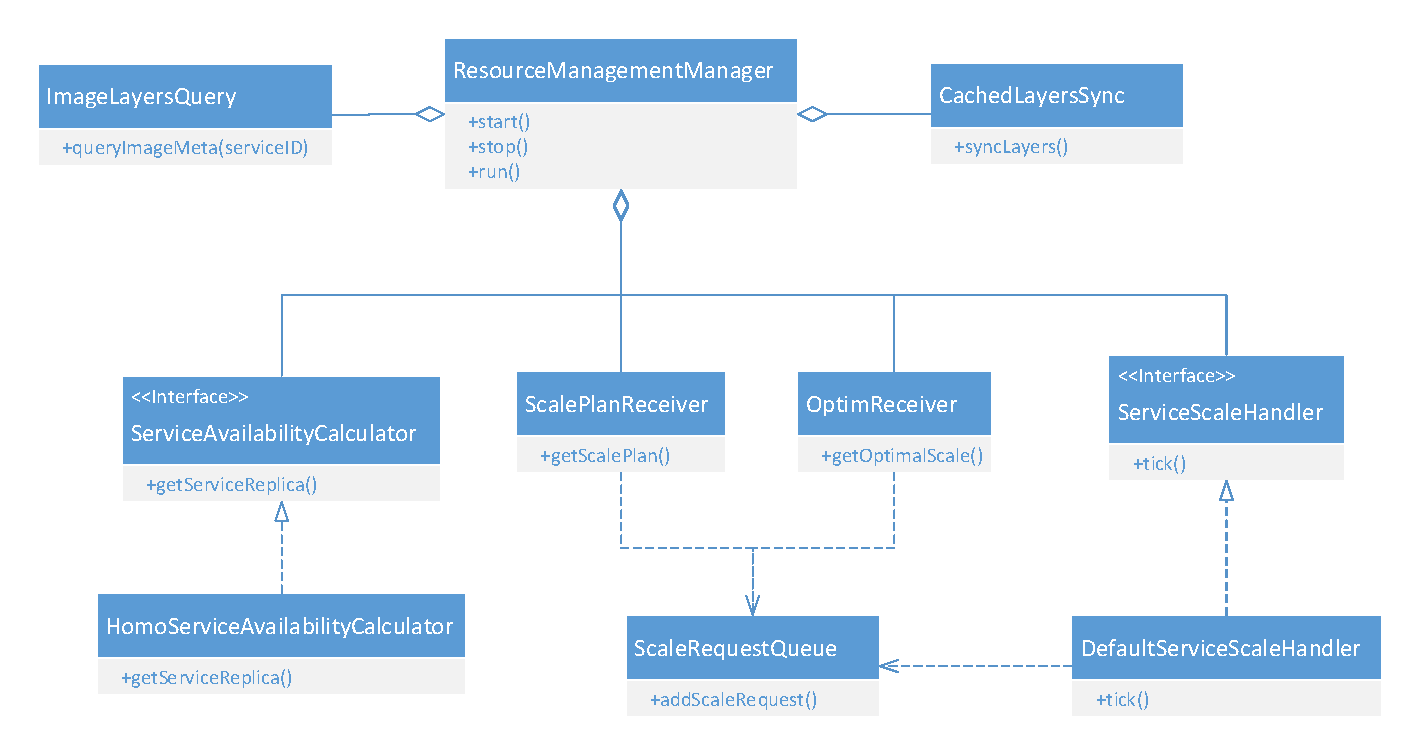
\includegraphics[width=0.9\textwidth]{./figure/manager_impl}
\bicaption[fig:manager-impl]{资源管理模块类图}{\textbf{资源管理模块类图}}{Fig}{Class Diagram for Resource Management Module}
\end{figure}
ResourceManagementManager类负责管理整个资源管理模块的运行周期。在资源管理模块中,ServiceAvailabilityCalculator接口通过getServiceReplica方法根据容器云中各节点的可用性指标和资源使用状态计算出服务需要的副本分布。本系统中ServiceAvailabilityCalculator接口的默认实现类为HomoServiceAvailabilityCalculator类,针对的是同构(即容器云中各节点的可用性指标都一样)的容器云,计算方法如设计中公式\ref{eq:replica}所示。ScalePlanReceiver类和OptimReceiver类分别通过getScalePlan方法和getOptimalScale方法从资源供给方案生成模块和资源供给优化模块利用gRPC接口获得相应的服务实例规模调整请求,并通过ScaleRequestQueue类的addScaleRequest方法将相应的实例规模调整请求数据添加到相应的等待队列中。ServiceScaleHandler接口通过tick方法周期性的对等待队列进行处理。DefaultServiceScaleHandler类将遍历等待队列中的所有服务伸缩请求,并按照其中时间戳数据的先后顺序,利用本系统中修改的Docker swarm服务伸缩API依次发起服务伸缩请求。此外,资源管理模块在处理服务创建请求的过程中,通过ImageLayersQuery类的queryImageMeta方法通过Docker \emph{registry} API获取服务运行所需Docker镜像中的层级文件信息,并保存在内存中供后续使用。CachedLayersSync类通过syncLayers方法,利用gRPC接口将各个工作者节点上的层级文件缓存信息按照增量的方式周期性地同步到工作者节点中。

\section{负载优化模块}
负载优化模块中的类结构设计如图\ref{fig:scheduler-impl}所示:
\begin{figure}[H]
\centering
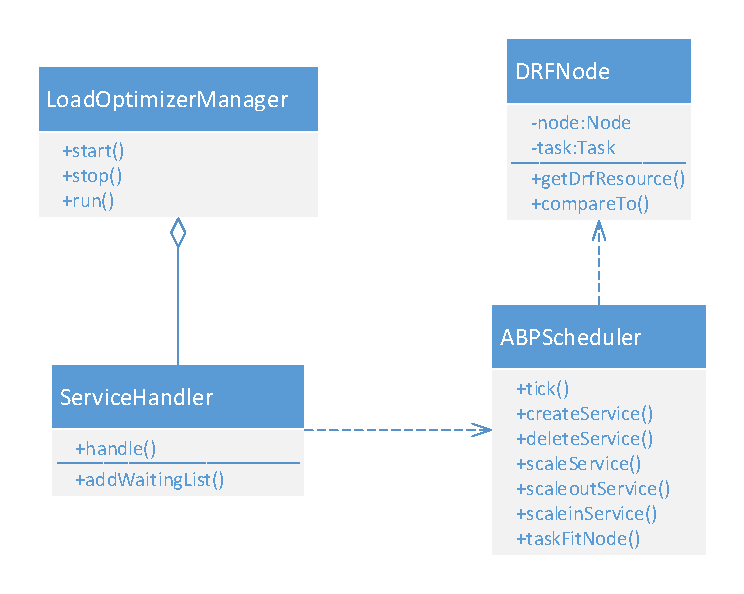
\includegraphics[width=0.9\textwidth]{./figure/scheduler_impl}
\bicaption[fig:scheduler-impl]{负载优化模块类图}{\textbf{负载优化模块类图}}{Fig}{Class Diagram for Load Optimazation Module}
\end{figure}
LoadOptimizerManager类负责管理整个负载优化模块的运行周期。ServiceHandler类负责从Docker swarm的API模块接收所有的服务相关的请求,包括服务的创建请求、销毁请求和伸缩请求,并通过handle方法对各个请求分析分拣,利用addWaitingList方法将服务实例规模相关的处理交给ABPScheduler类完成。ABPScheduler类对收到的所有服务变更请求放入等候队列中,通过tick方法周期性地对等候队列中的所有服务变更请求进行处理。根据服务请求的类型,ABPScheduler类利用createService方法来负责处理服务的创建请求,通过deleteService方法来负责处理服务的销毁请求,用scaleService方法来负责处理服务的伸缩请求。ABPScheduler类在scaleService方法中对当前服务的实例规模和请求的实例规模进行对比:如果请求的实例数超过当前实际的实例数,则ABPScheduler类通过scaleoutService方法对相应服务进行扩展;如果如果请求的实例数少于当前实际的实例数,ABPScheduler类就使用scaleinService方法对相应服务进行收缩;如果实例数要求不变,则抛弃此次调整请求。在ABPScheduler中,我们利用taskFitNode方法来判断一个集群节点是否满足任务实例运行的需要。DRFNode类表示一个可能的任务节点组,其中利用getDrfResource方法可以获得该任务节点组的优势资源,基于启发式的多优先级规则在compareTo方法中重新定义DRFNode对象的优先级比较方法。

\section{本章小结}
本章通过类图的方式详细介绍了本文所实现系统中各个模块的具体实现方式。由于本文提出的系统是一个分布式系统,因此我们引入了大量的异步操作和批处理操作,从而实现提高系统整体吞吐量和健壮性的目标。在具体实现过程中,我们将整体的可扩展性和可维护性作为重要目标,使得我们实现的系统可以在后续的工作中进行进一步地完善和发展,让用户根据自身的需求进行自主化定制成为可能。
%# -*- coding: utf-8-unix -*-
%%==================================================
%% chapter01.tex for SJTU Master Thesis
%%==================================================

%\bibliographystyle{sjtu2}%[此处用于每章都生产参考文献]
\chapter{系统实验与验证}\label{chap:sys_eval}
在本章中,我们对本文提出的主动式容器云资源管理模型进行实验验证,并对实验结果进行必要的分析和说明。本文提出的模型可以分为负载监测和预测、资源供给和管理以及负载应对这三个部分。由于本文的最终目标是提高容器云应对负载变化的响应能力,优化的方法主要分为基于预测的主动式调整和对任务实例分发调度策略的优化,资源供给部分主要职责是根据预测和观测的资源使用量确认实例规模大小,并没有任何优化的功能,因此我们验证的重点也主要是在负载预测的准确性和引入的新任务实例调度策略对容器云中任务实例分发管理的影响。在负责预测部分的实验中,我们根据实验得出相关模型的预测正确率和预测偏差率等数据,利用这两个量化标准来说明相应模型实际的预测效果;在负载优化部分的实验中,为了对本文提出的模型进行验证,我们利用Docker \emph{swarm}作为容器云的比较对象,并通过服务创建和服务伸缩的方法对本文实现的系统进行了相关实验。

\section{实验环境设定}\label{sec:env_prep}
为了验证系统的有效性,本课题对整体的硬件和软件环境进行了相关准备,具体设定如下所示:
\begin{enumerate}
\item 我们使用4台Dell R420机架式服务器作为容器集群的托管服务器,利用Docker swarmkit作为底层容器集群实现,构建基于Docker的容器云。每台服务器有4个CPU核心,内存大小为8GB,详细的服务器硬件配置参数如表\ref{tb:machine_perf}所示。

\begin{table}[h]
\centering
\bicaption[tb:machine_perf]{物理服务器性能参数}{物理服务器性能参数}{Table}{Physical Server's Technical Specification}
\begin{tabular}{@{}lr@{}} \toprule
 资源类型 & 性能参数 \\ \midrule
 CPU型号 & Intel Xeon E5-2650\\
 CPU核心数 & 4\\
 内存大小 & 8G\\
 内网出入带宽 & 2Gbps\\
 外网出入带宽 & 100Mbps\\ \bottomrule
\end{tabular}
\end{table}

\item 整个容器集群利用上述4台服务器构成4个集群节点,包括1个管理者节点(manager)和3个工作者节点(worker)。在试验中,我们假定每台服务器的可用性指标保持一致,均为0.9,因此容器集群中每个节点的可用性也都保持一致。这意味着对同一个服务而言,任务在容器集群内任一节点上对服务的整体可用性的影响是一样的。

\item 在负载预测部分的实验中,我们使用1998年世界杯网站的流量数据作为模拟的系统负载数据,通过对该流量数据的预测结果来验证预测模块的有效性。该数据包含了从1998年4月30日到1998年7月26日之间世界杯网站的访问请求记录,并且被广泛应用在了时序数据处理相关领域中,流量整体趋势如图\ref{fig:load_trend}所示:
\begin{figure}[htbp]
\centering
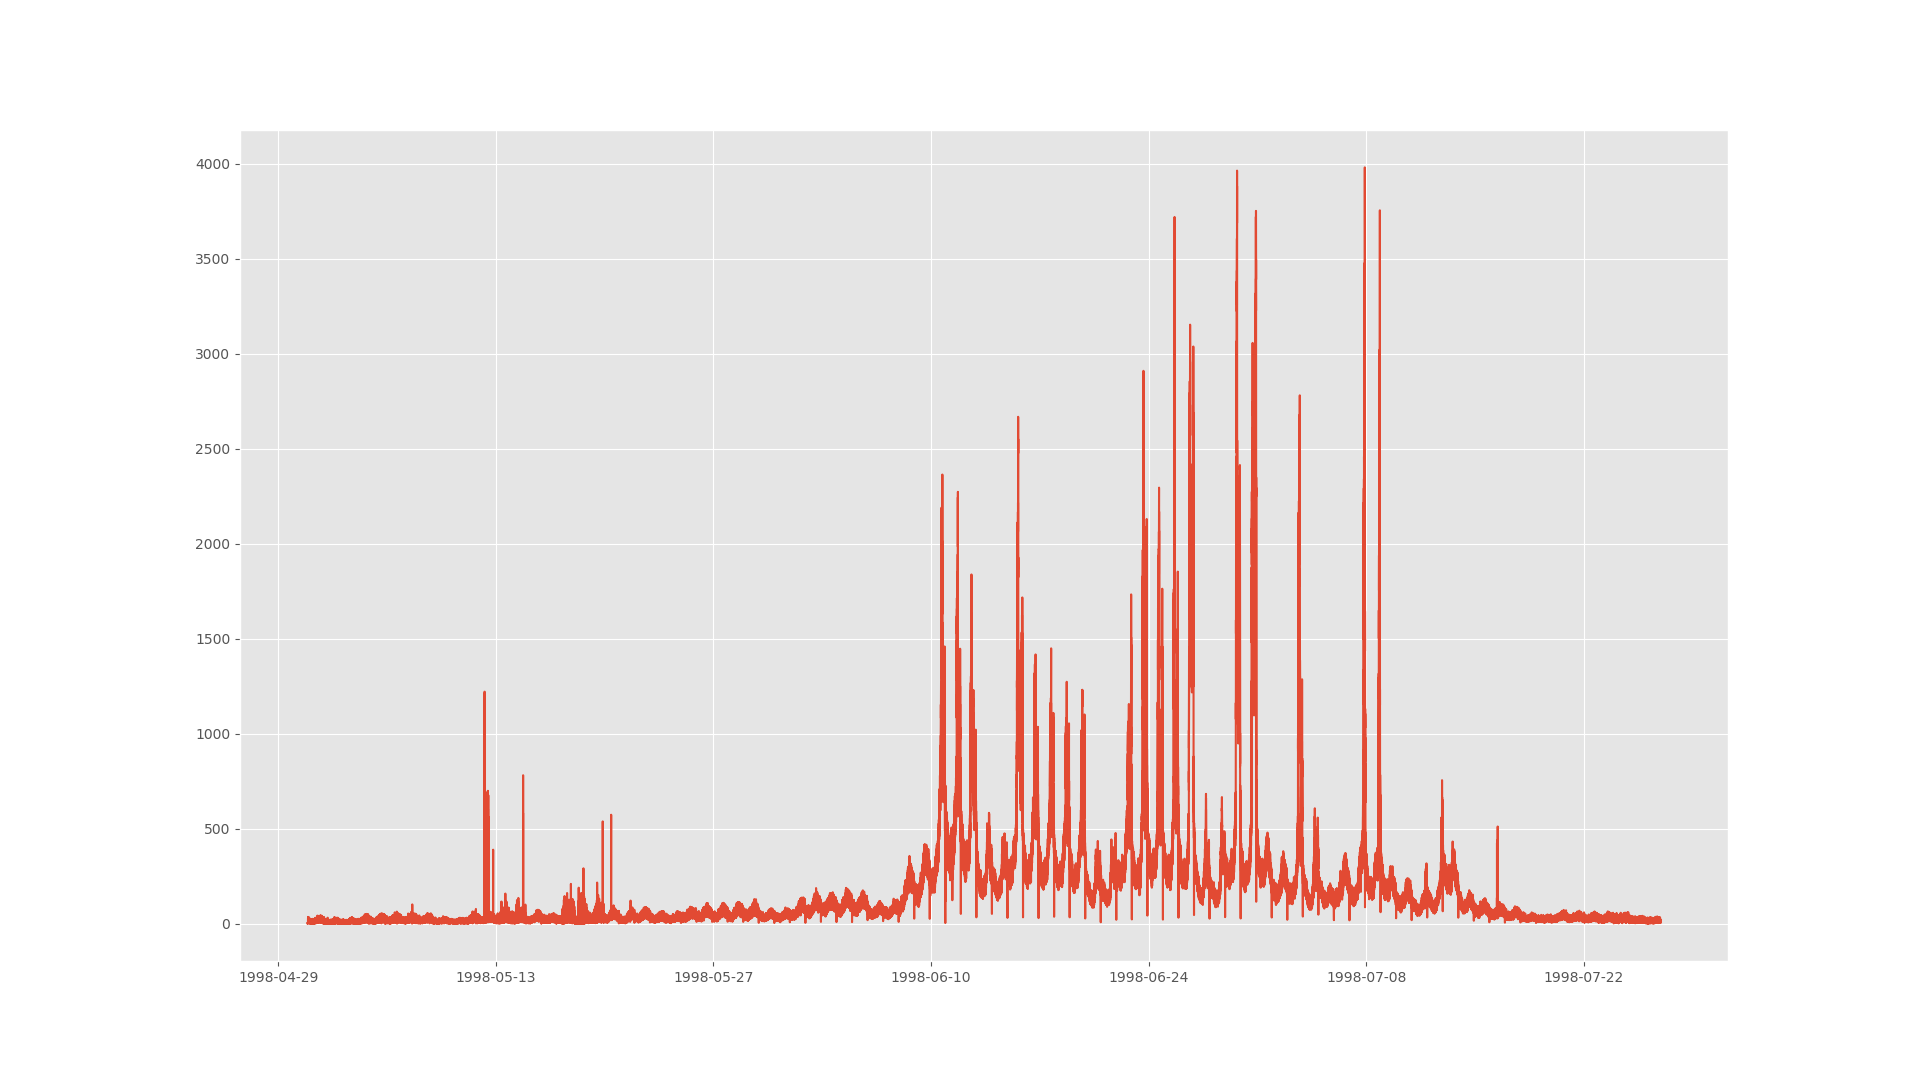
\includegraphics[width=0.9\textwidth]{./figure/alldata}
\bicaption[fig:load_trend]{98年世界杯网站整体流量趋势}{\textbf{98年世界杯网站整体流量趋势}}{Fig}{The load trend of 98' World Cup Site}
\end{figure}

\item\label{req:serv_image} 我们分别以Docker Hub上提供的官方\emph{debian:jessie}镜像和官方\emph{ubuntu:xenial}镜像为基础,通过依赖包安装的方式安装好\emph{Golang}的运行时环境(约270MB大小),构建两个不同的基础镜像\emph{base1}和\emph{base2}。我们分别基于这两个基础镜像对同一个\emph{Golang}应用构建两个不同的应用镜像\emph{image1}和\emph{image2}。除此之外,我们利用官方\emph{debian:jessie}镜像作为基础镜像,对shell应用构建了第三个应用镜像\emph{image3}。\emph{image1}和\emph{image3}都包含基础镜像\emph{debian:jessie},因此镜像\emph{image1}和镜像\emph{image3}中来自\emph{debian:jessie}镜像的层级文件可以被这两个镜像共享,这就意味着在同一个节点,只需要下载一次\emph{debian:jessie}镜像,那相应的层级文件就能被镜像\emph{image1}和镜像\emph{image3}共享而不需要额外的下载。

\item 为了减少网络延迟和网络稳定性对试验的影响,我们选择使用Docker镜像的本地二进制文件安装方式来安装和配置依赖环境,而不是用诸如apt、yum等常见的依赖配置管理工具从网络上的官方二进制仓库来获取和安装相关依赖。

\item\label{req:serv_aval} 针对上述三个不同的应用镜像,我们在容器云中分别部署了三个不同的服务,分别命名为\emph{service1},\emph{service2}和\emph{service3},每个服务默认占用0.5个CPU核心和1GB的内存资源。每个服务指定的服务可用性目标是0.99。根据等式, 每个服务应该配置2个副本以满足服务可用性目标。

\item\label{req:registry_mirror} 为了减少网络传输的延迟,加快容器云整体的容器镜像分发速度,我们在实验环境下搭建了一个Docker \emph{registry}镜像来对镜像文件进行缓存和下载加速。Docker容器集群和Docker \emph{registry}服务之间通过百兆网络进行连接。容器集群中的各节点在下载镜像时可以利用本地搭建的Docker \emph{registry}服务进行下载,而避免直接从Docker Hub获得镜像导致的额外网络传输开销。

\item 为了获取更可信的数据,我们对每个实验项目进行三次独立实验,对测得实验数据去平均值作为该实验项目的观测值。在每次实验结束后,我们都将重启集群节点上的Docker Engine并重置整个实验环境,以避免下一次的实验收到本次实验过程的影响。
\end{enumerate}

\section{系统负载预测部分验证和分析}
由图\ref{fig:load_trend}中可以看出,流量的变化主要和比赛日时间有关,诸如工作日等日常的时间标志对流量变化的影响很小。比赛日之间的流量变化模式比较近似,而且在若干时间段内存在流量急速增加和迅速降低的场景。除此之外,通过对原始数据的分析,我们还发现每天不同时间段流量的变化基本是相似的。1998年世界杯的比赛日程为1998年6月10日到1998年7月12日,我们从中选取了6月16日到7月9日之间世界杯网站的部分流量数据作为本次实验的测试数据集,并给出基于自回归滑动平均模型的预测算法和基于长短期记忆模型的预测算法在相应数据上的预测评估结果。

\subsection{自回归滑动平均模型的预测实验}\label{sec:arima_eval}
在基于自回归滑动平均模型的预测算法中,我们维护了一个4天的时间窗口。由于基于自回归滑动平均模型的预测计算量随着时间窗口的增加而增加,我们将5分钟之内的资源使用状态进行汇总并计算出下一个周期的资源使用量预测。我们根据基于自回归滑动平均模型的预测算法,对6月18日到6月19日之间、6月24日当天、7月8日到7月9日之间和7月11日到7月13日期间的流量数据进行预测,最终预测效果如图\ref{fig:arma_algo}所示:
\begin{figure}[htbp]
\centering
\subfigure[6月18日到6月19日]{
    \label{fig:arma_algo:5255}
    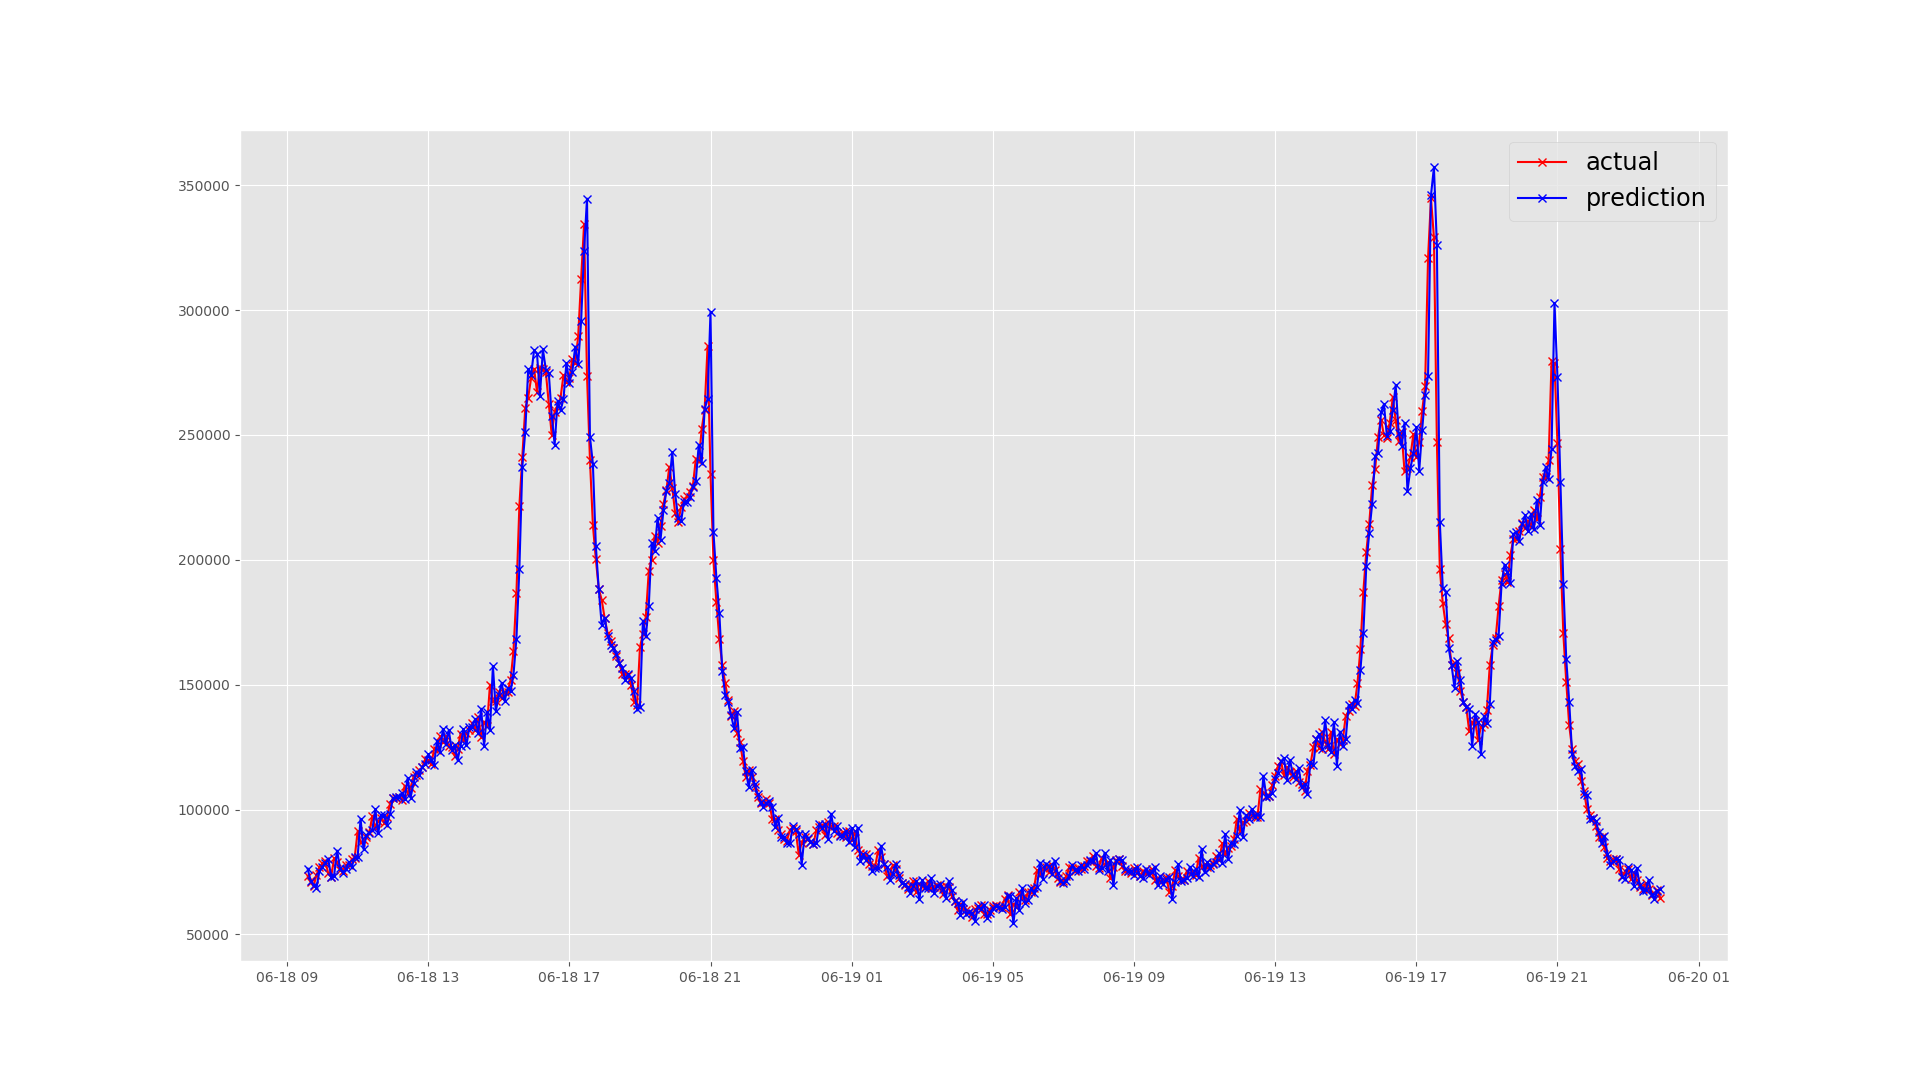
\includegraphics[width=0.45\textwidth]{./figure/arma5255}}
\subfigure[6月24日]{
    \label{fig:arma_algo:5961}
    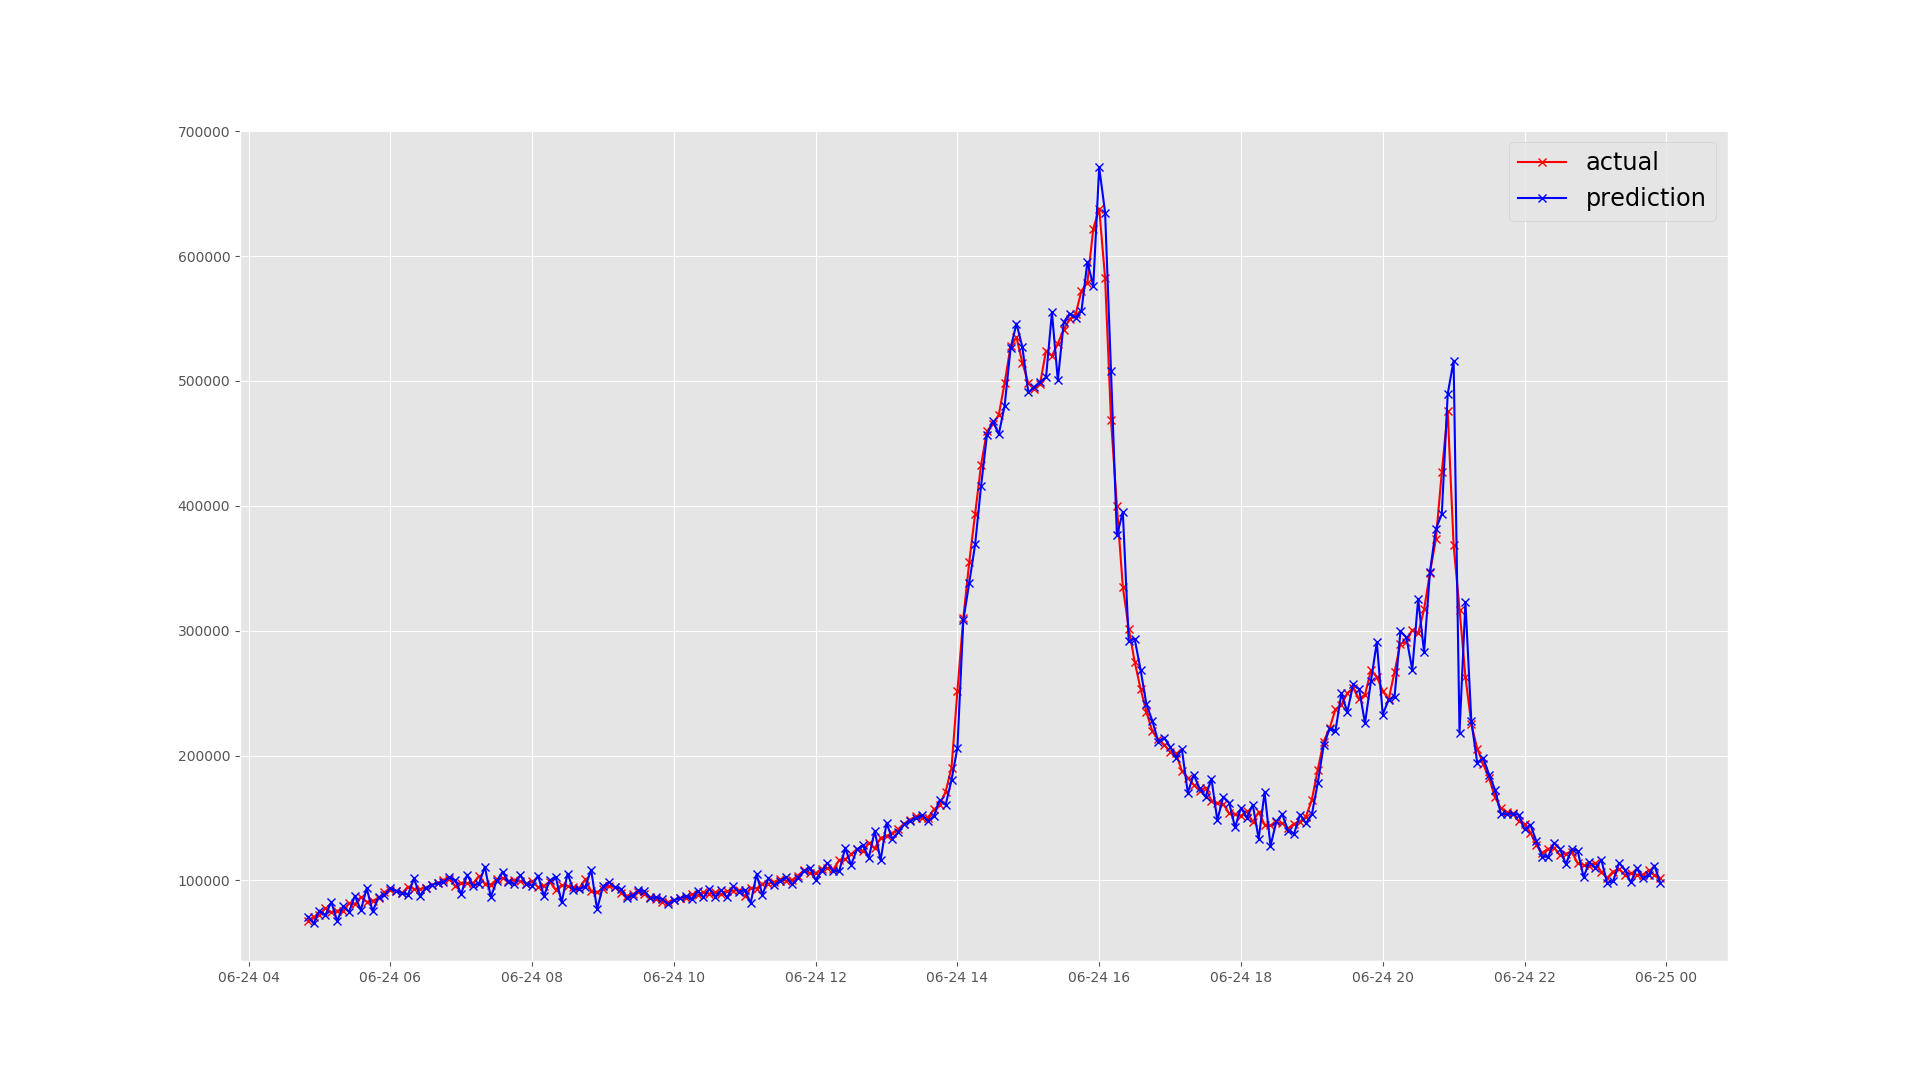
\includegraphics[width=0.45\textwidth]{./figure/arma5961}}
\subfigure[7月8日到7月9日]{
    \label{fig:arma_algo:7376}
    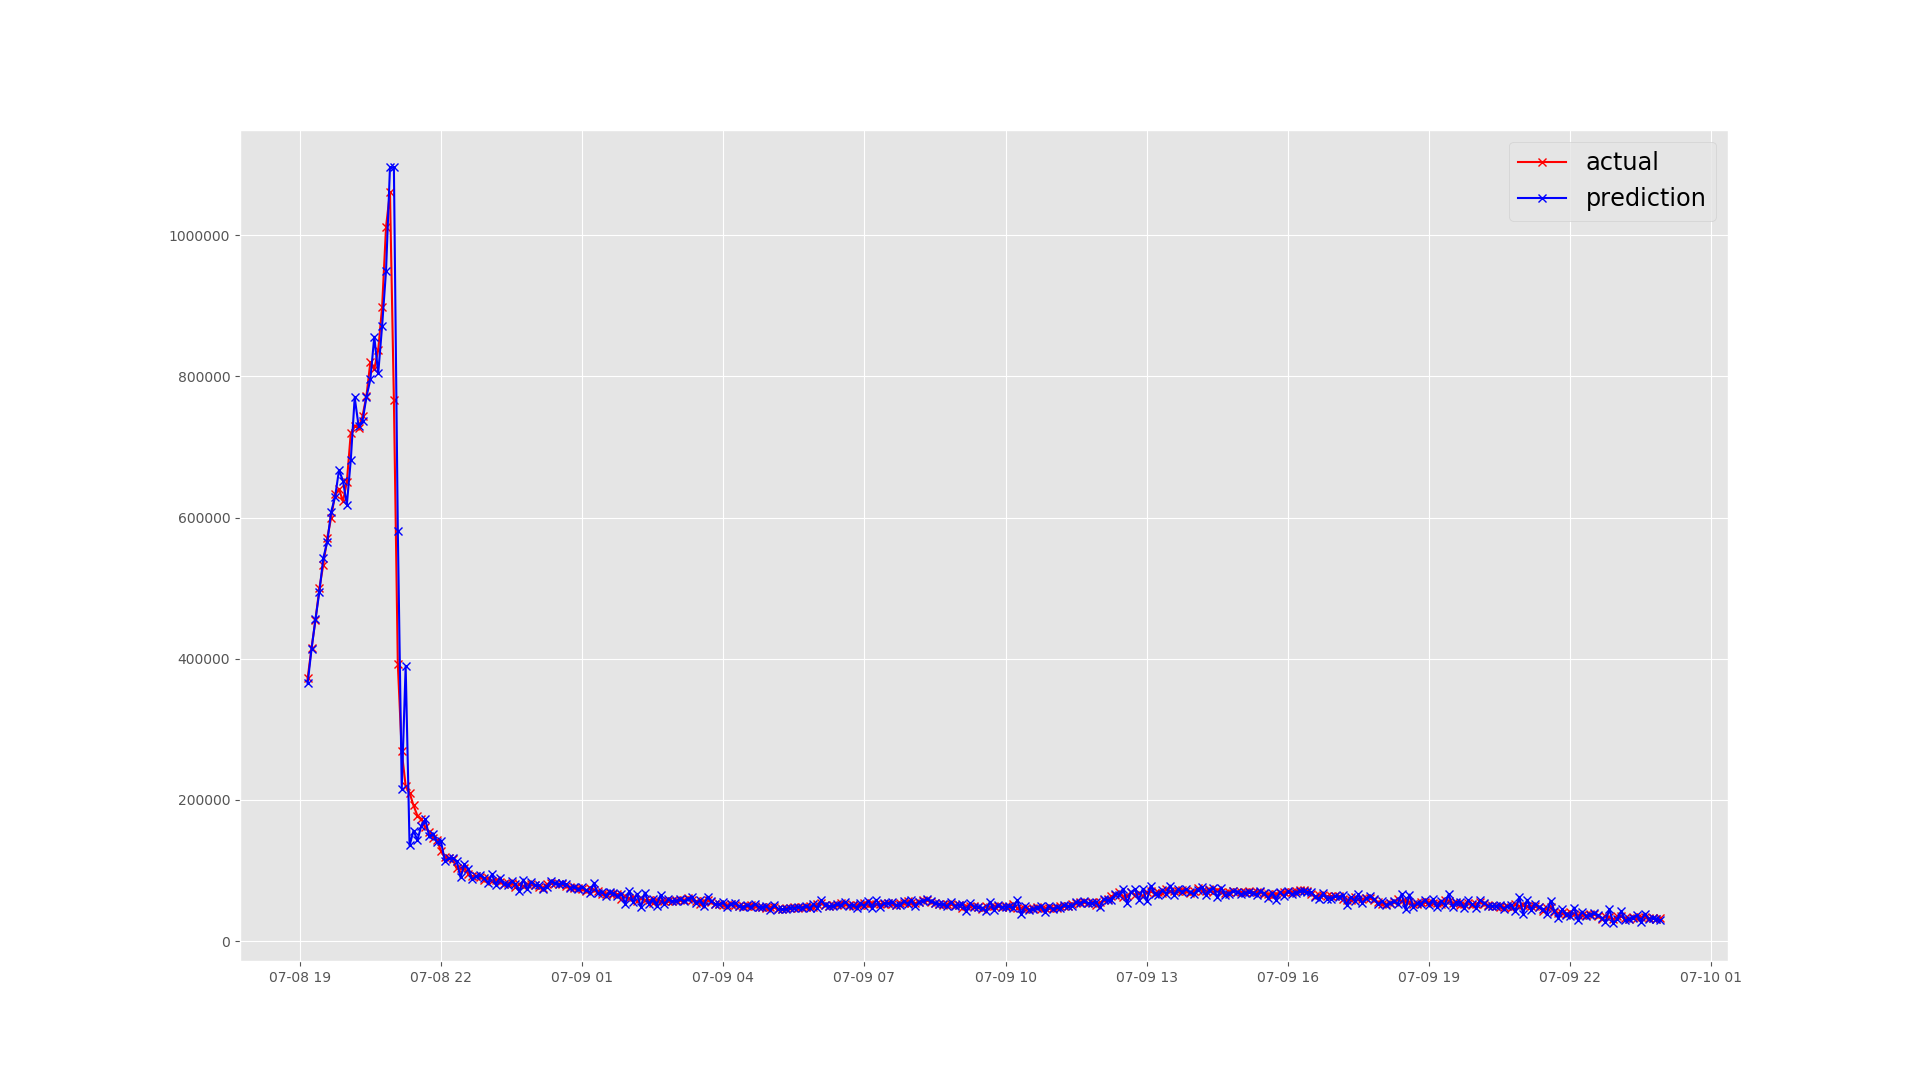
\includegraphics[width=0.45\textwidth]{./figure/arma7376}}
\subfigure[7月11日到7月13日]{
    \label{fig:arma_algo:7379}
    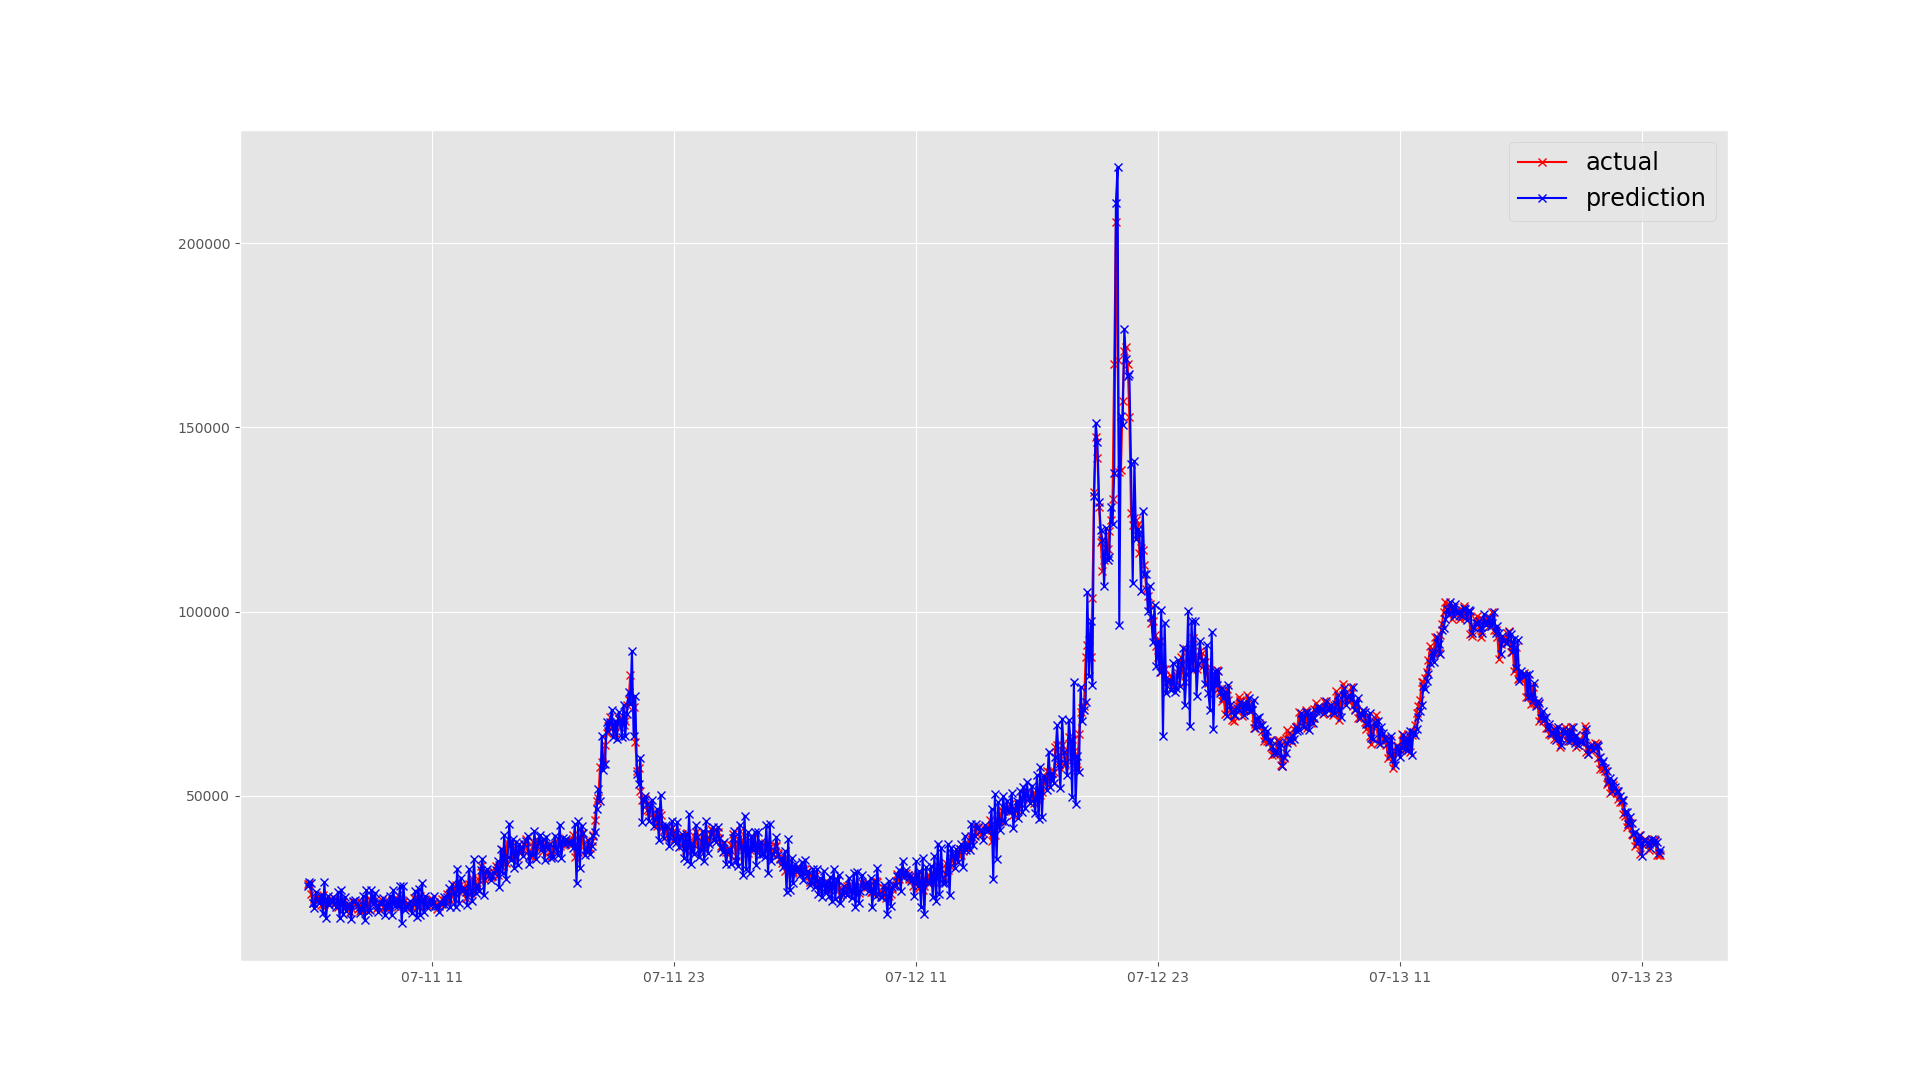
\includegraphics[width=0.45\textwidth]{./figure/arma7379}}
\bicaption[fig:arma_algo]{基于ARIMA模型的预测}{基于ARIMA模型的预测结果}{Fig}{The load prediction of ARIMA}
\end{figure}

表\ref{tb:arma}从预测正确率、预测偏差率和预测偏方差率这三个角度显示了基于ARIMA模型的预测算法对四个不同时间段内流量的实际预测结果,
\begin{table}[h]
\centering
\bicaption[tb:arma]{基于ARIMA模型的预测算法评估}{基于ARIMA模型的预测算法评估}{Table}{The precision of prediction for loads based on ARIMA model}
\begin{tabular}{@{}lcccc@{}}\toprule
  & 6.18到6.19 & 6.24 & 7.8到7.9 & 7.11到7.13 \\ \midrule
 预测正确率 & 47.9\% & 45.2\% & 48.0\% & 49.1\% \\
 预测偏差率 & 3.7\% & 5.2\% & 7.0\% & 7.2\% \\
 预测偏方差率 & 7.5\% & 10.3\% & 14.2\% & 14.4\% \\ \bottomrule
\end{tabular}
\end{table}
由表\ref{tb:arma}可知,


\subsection{基于长短期记忆模型的预测实验}\label{sec:lstm_eval}


\begin{figure}[htbp]
\centering
\subfigure[6月18日到6月19日]{
    \label{fig:lstm_algo:5255}
    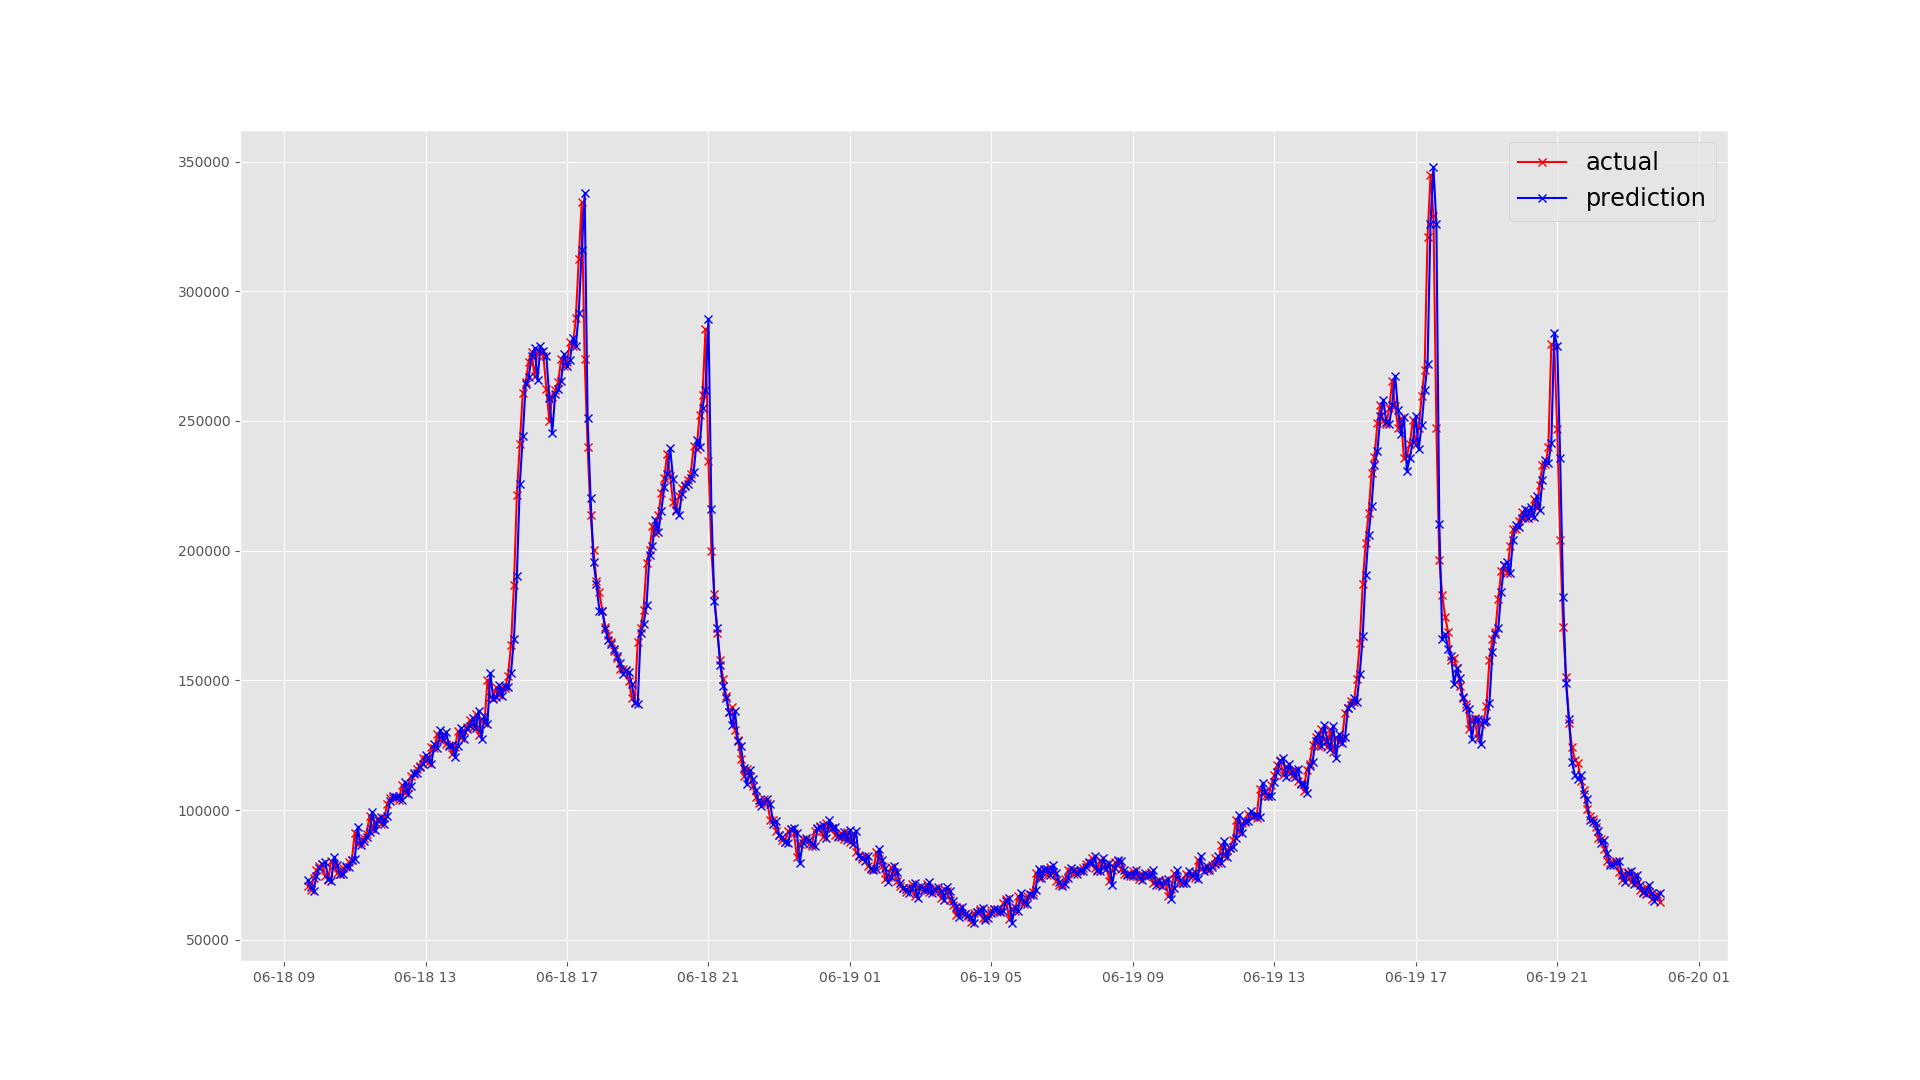
\includegraphics[width=0.45\textwidth]{./figure/lstm5255}}
\subfigure[6月24日]{
    \label{fig:lstm_algo:5961}
    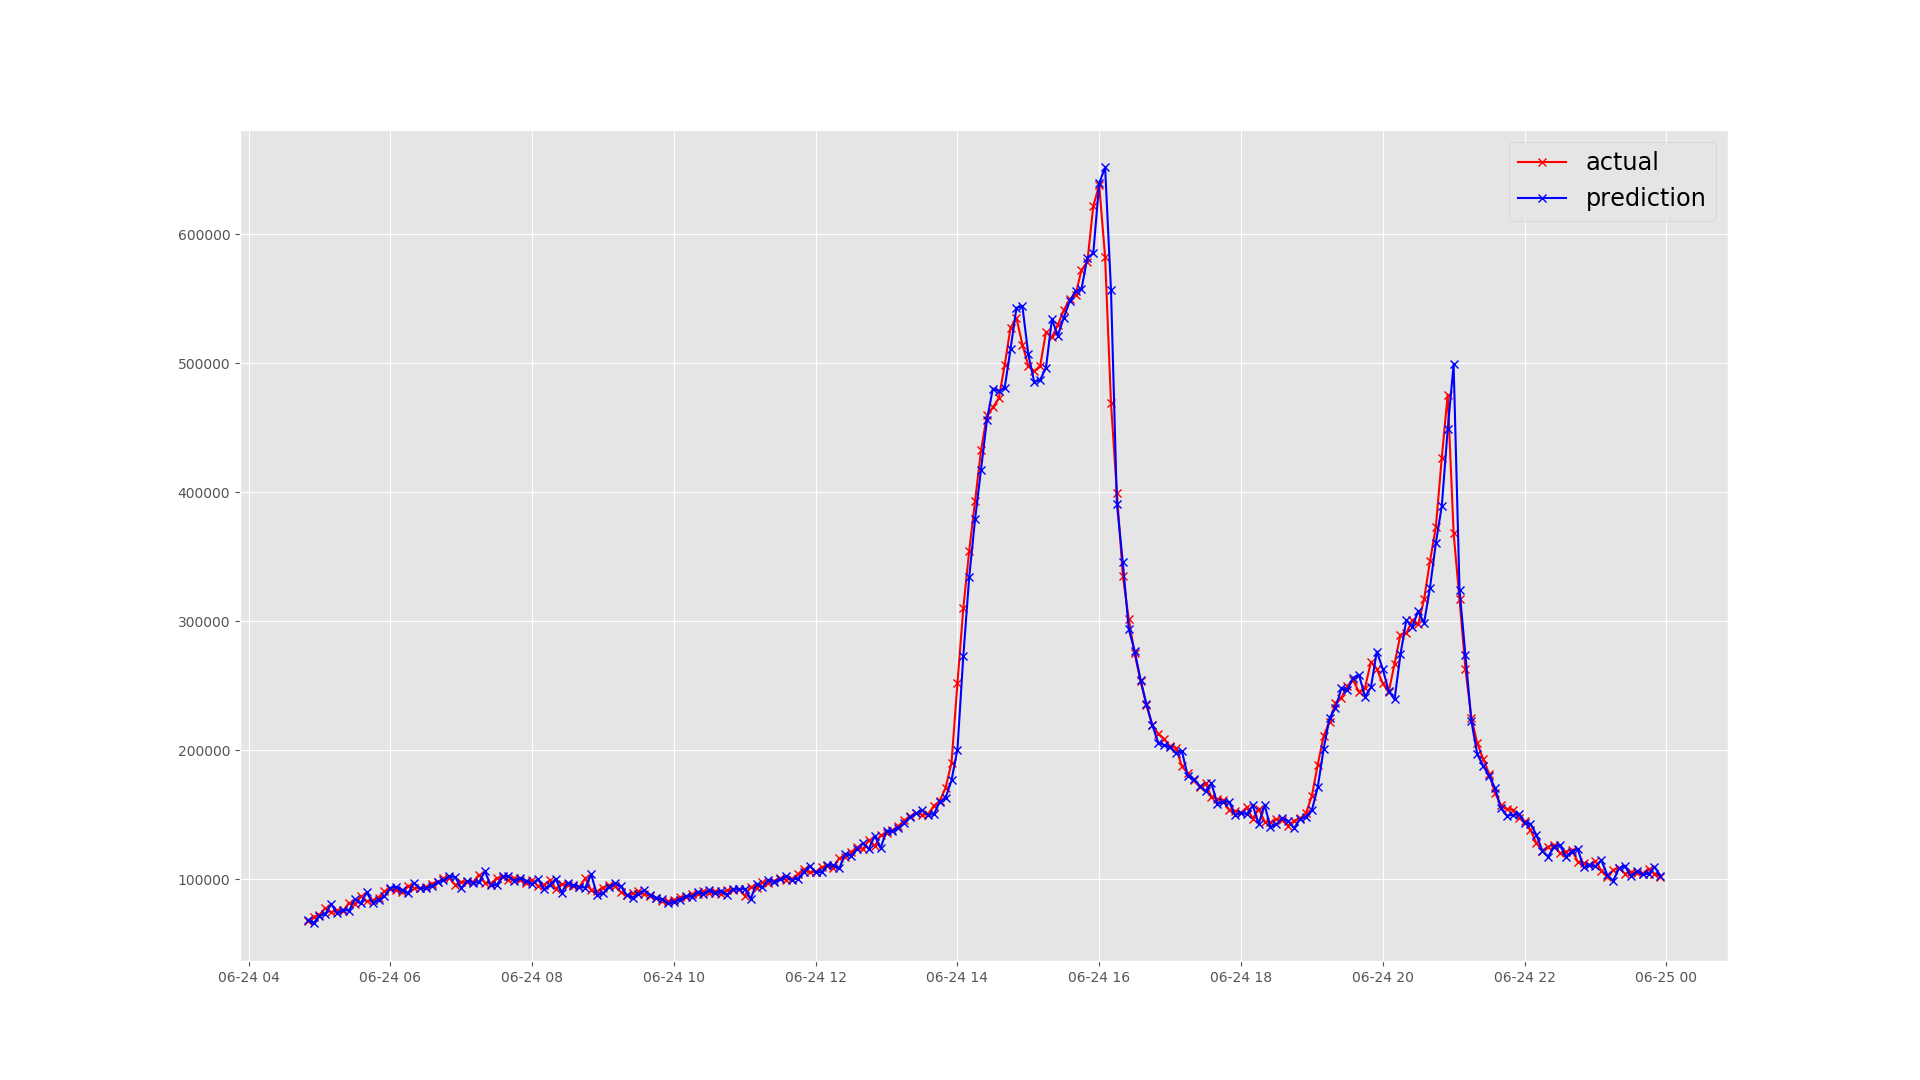
\includegraphics[width=0.45\textwidth]{./figure/lstm5961}}
\subfigure[7月8日到7月9日]{
    \label{fig:lstm_algo:7376}
    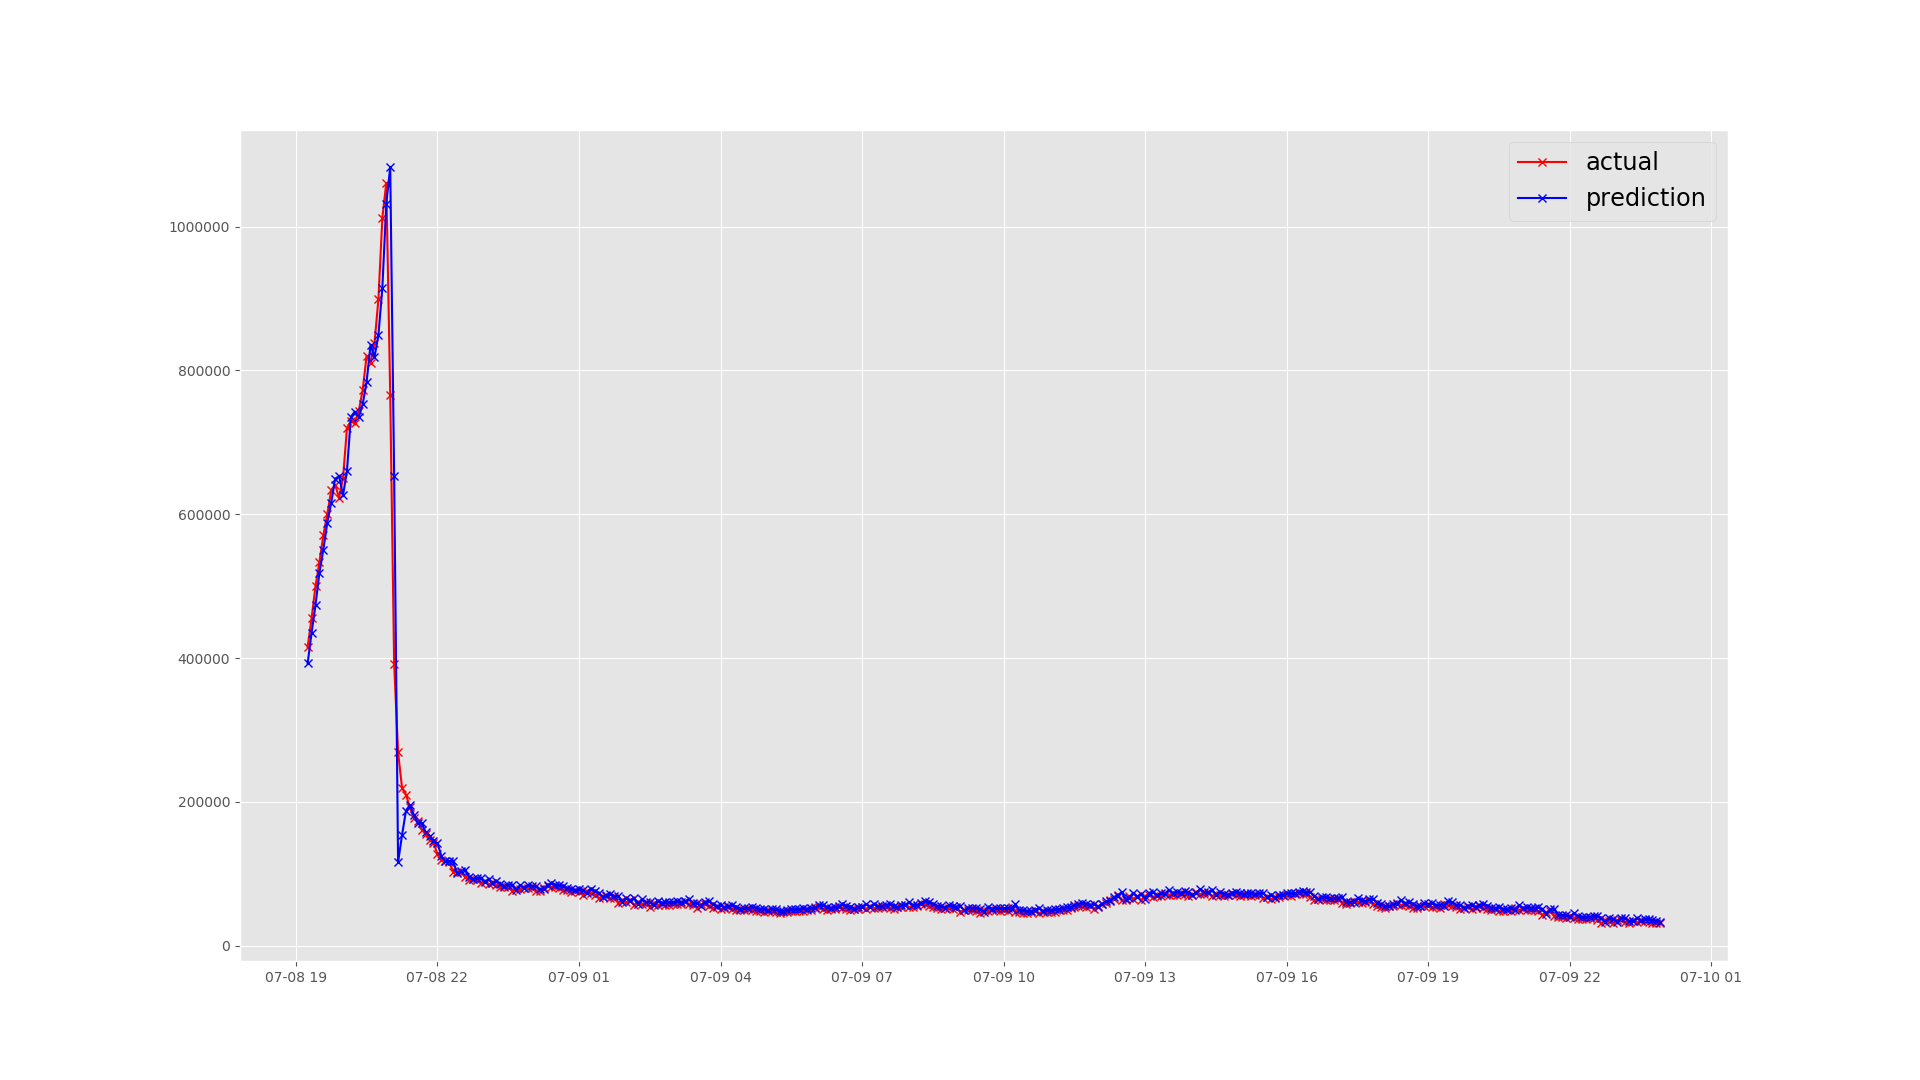
\includegraphics[width=0.45\textwidth]{./figure/lstm7376}}
\subfigure[7月11日到7月13日]{
    \label{fig:lstm_algo:7379}
    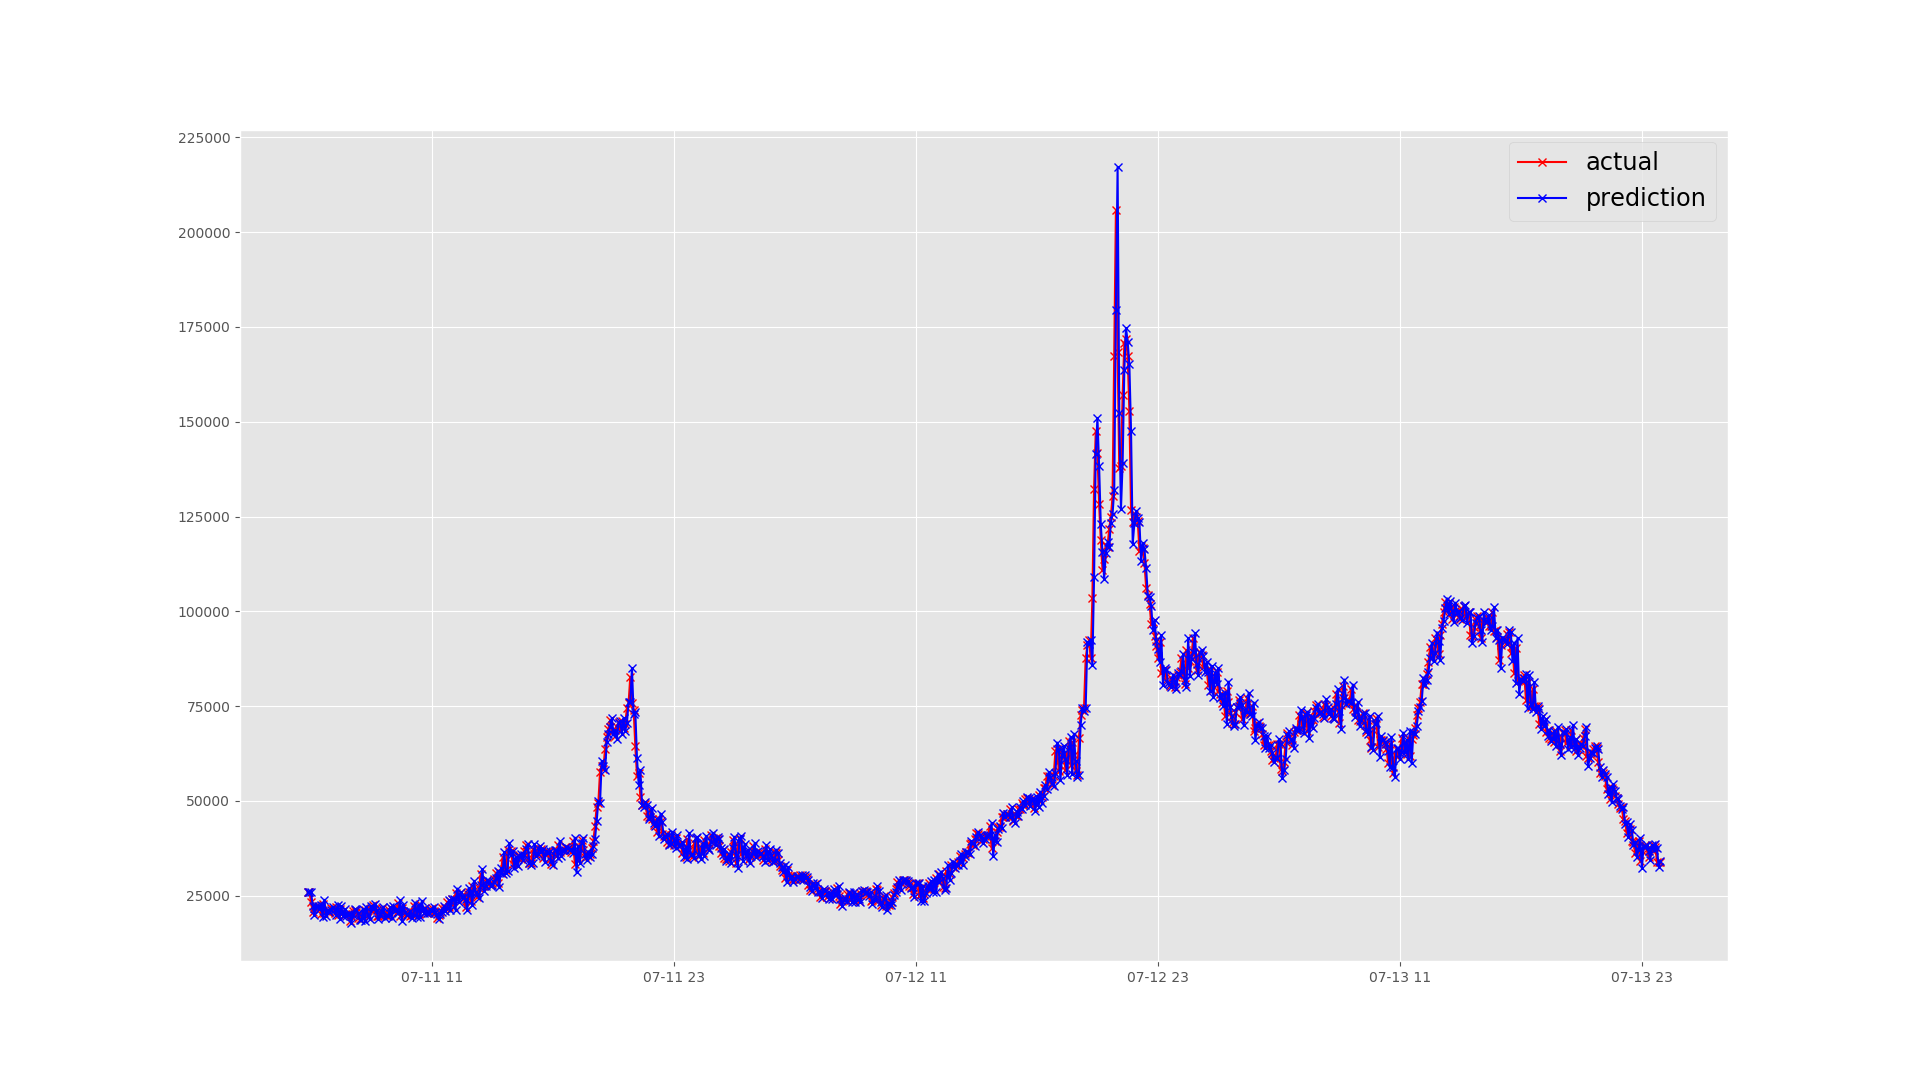
\includegraphics[width=0.45\textwidth]{./figure/lstm7379}}
\bicaption[fig:lstm_day]{基于LSTM模型的预测}{基于LSTM模型的预测结果}{Fig}{The load prediction of LSTM}
\end{figure}


\begin{table}[h]
\centering
\bicaption[tb:lstm]{基于LSTM模型的预测算法评估}{基于LSTM模型的预测算法评估}{Table}{The precision of prediction for loads based on LSTM model}
\begin{tabular}{@{}lcccc@{}}\toprule
  & 6.18到6.19 & 6.24 & 7.8到7.9 & 7.11到7.13 \\ \midrule
 预测正确率 & 44.1\% & 42.2\% & 83.8\% & 49.6\% \\
 预测偏差率 & 3.4\% & 3.5\% & 6.6\% & 4.8\% \\
 预测偏方差率 & 6.8\% & 7.1\% & 13.8\% & 9.5\% \\ \bottomrule
\end{tabular}
\end{table}

\section{负载优化部分实验结果和分析}
本课题主要目标是使容器云能够更加快速的相应变化的负载,因此除了通过上述的预测来进行提前准备之外,还需要对实时变化的负载进行应对,避免因为预测错误而导致响应延迟降低整体的服务质量。为了验证本课题所提出提出模型的有效性,我们分别从服务的创建延迟和伸缩延迟两个方面进行实验和分析。

\subsection{服务创建实验}\label{sec:serv_creation}
我们分别使用Docker \emph{swarm}和本课题实现的系统就容器集群中服务创建的过程展开实验。我们针对在容器云中创建服务的测试设计了三个不同的测试场景,并按照\ref{req:serv_aval}中的要求基于应用镜像\emph{image1}、\emph{image2}和\emph{image3}分别创建\emph{service1},\emph{service2}和\emph{service3}这三个服务:
\begin{enumerate}
\item\label{create1} 分别用Docker \emph{swarm}和本文提出的系统创建服务\emph{service1},\emph{service2}和\emph{service3}。每个服务有2个任务实例,同时为了满足\ref{req:serv_aval}中提到的可用性要求,在本课题提出的系统中为每个服务设置2个副本。
\item\label{create2} 分别用Docker \emph{swarm}和本文提出的系统依次创建服务\emph{service1},\emph{service2}和\emph{service3}。每个服务有4个任务实例,同时为了满足\ref{req:serv_aval}中提到的可用性要求,在本课题提出的系统中为每个服务设置2个副本。
\item\label{create3} 分别用Docker \emph{swarm}和本文提出的系统按照\emph{service1},\emph{service3}和\emph{service2}的顺序依次创建服务。每个服务有2个任务实例,同时为了满足\ref{req:serv_aval}中提到的可用性要求,在本课题提出的系统中为每个服务设置2个副本。
\end{enumerate}

\begin{figure}[htbp]
\centering
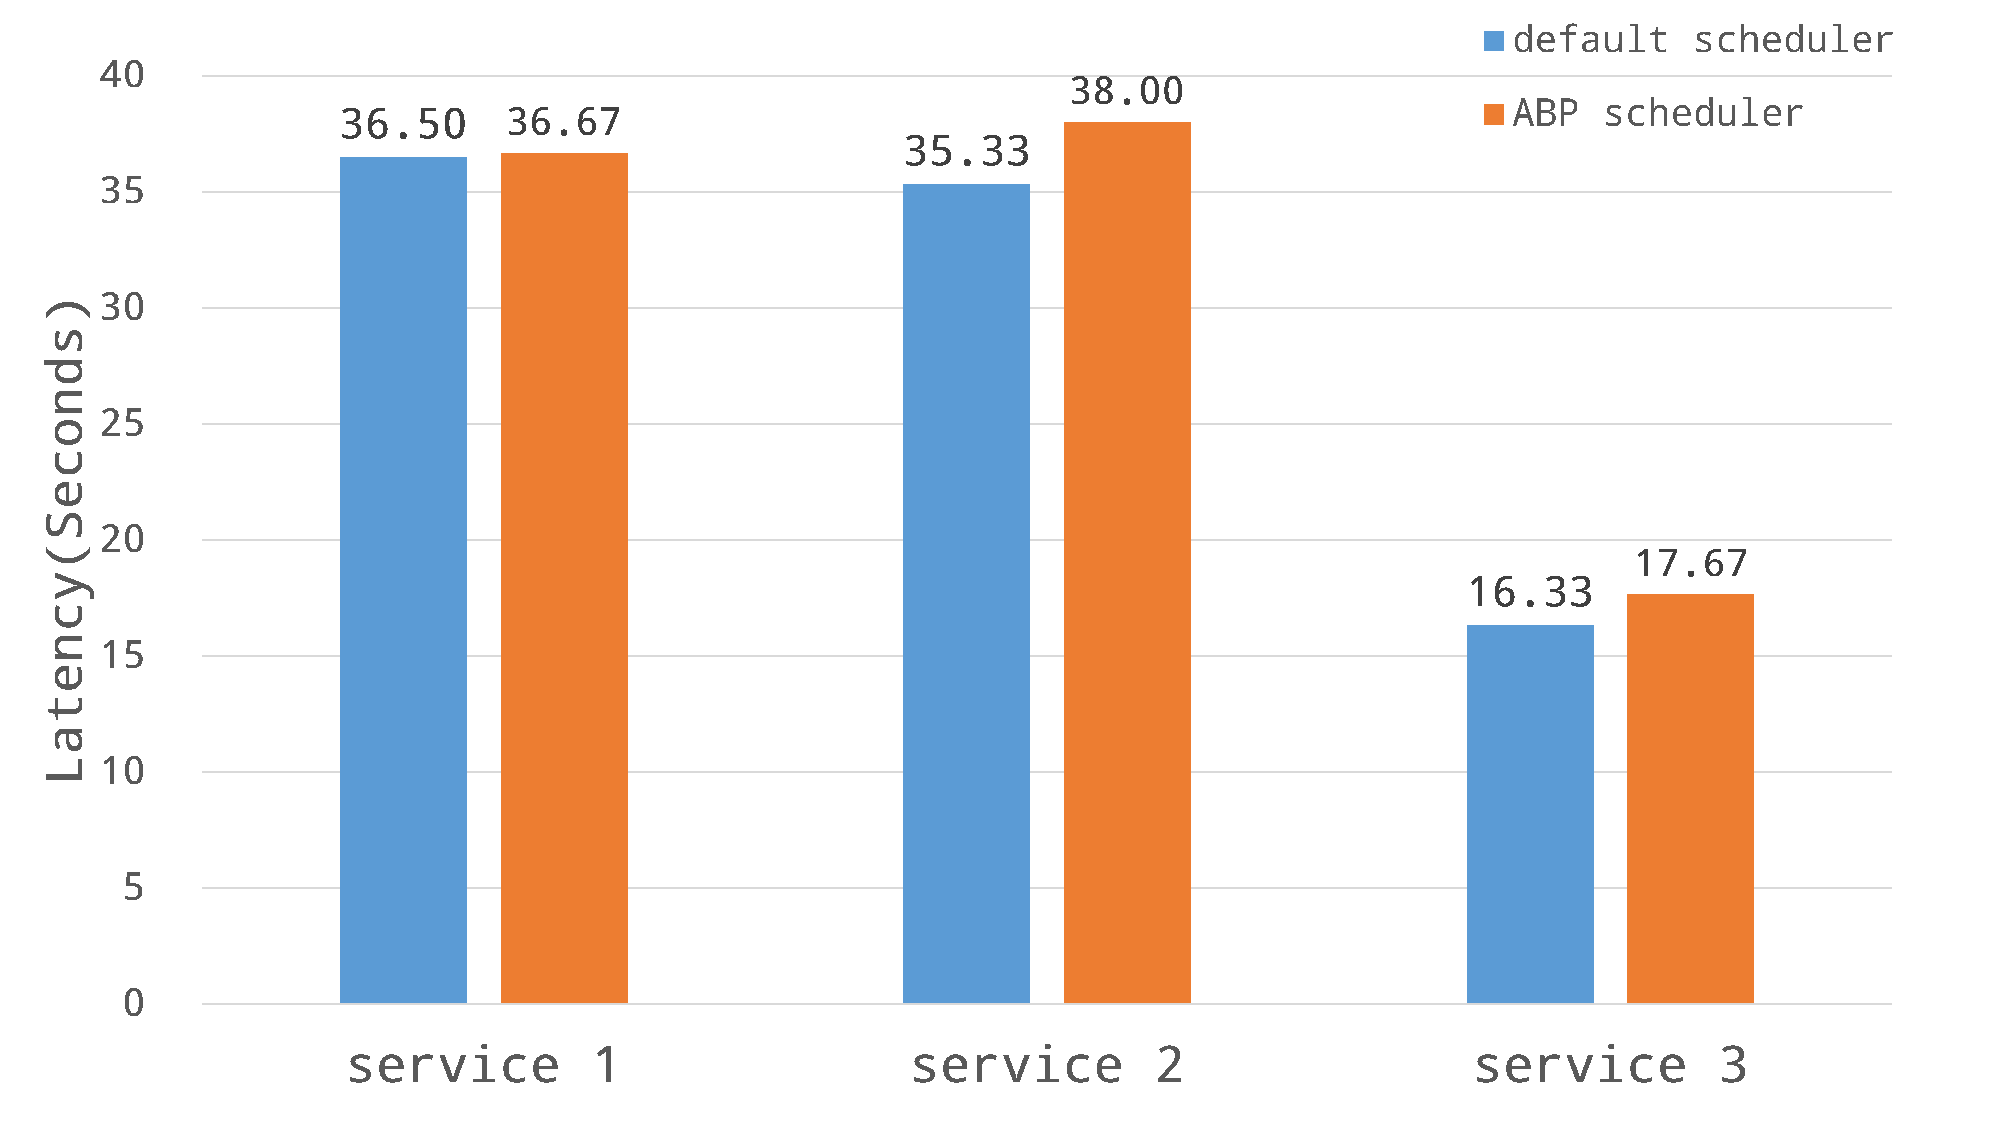
\includegraphics[width=0.9\textwidth]{./figure/baseline}
\bicaption[fig:baseline]{创建服务耗时基准}{\textbf{服务创建耗时}: 以每个服务的副本数要求为2且有2个任务实例作为本次实验的基准}{Fig}{\textbf{Services Creation}: creating each service with 2 tasks and 2 replicas, as the baseline of our experiments}
\end{figure}

我们将测试场景\ref{create1}中的测试结果作为衡量不同系统在容器云集群中创建启动相应服务所需耗时的基准值。从图\ref{fig:baseline}中可以看出,相关服务在本课题的系统中启动耗时相比默认的Docker \emph{swarm}框架要略微高一些。这是由于相比Docker \emph{swarm},本课题提出的系统需要额外从Docker \emph{registry}(并非本地的Docker \emph{registry}镜像服务)获取Docker镜像文件的元数据造成的耗时。但由于镜像元数据的数据量很小,因此这个额外耗时主要消耗在建立网络连接过程,根据实验过程中的多次测试验证,整个过程耗时很少超过3秒。对比下载整个镜像文件的耗时造成的延迟损失,我们认为这部分的延迟开销是可以接受的。除此之外,通过对实验观测到的数据进行分析,我们发现本系统的标准差比Docker \emph{swarm}框架中的标准差高出1秒左右,这主要是由于从国内实验环境连接到位于美国的Docker \emph{registry}服务的网络环境不稳定导致的。

\begin{figure}[htbp]
\centering
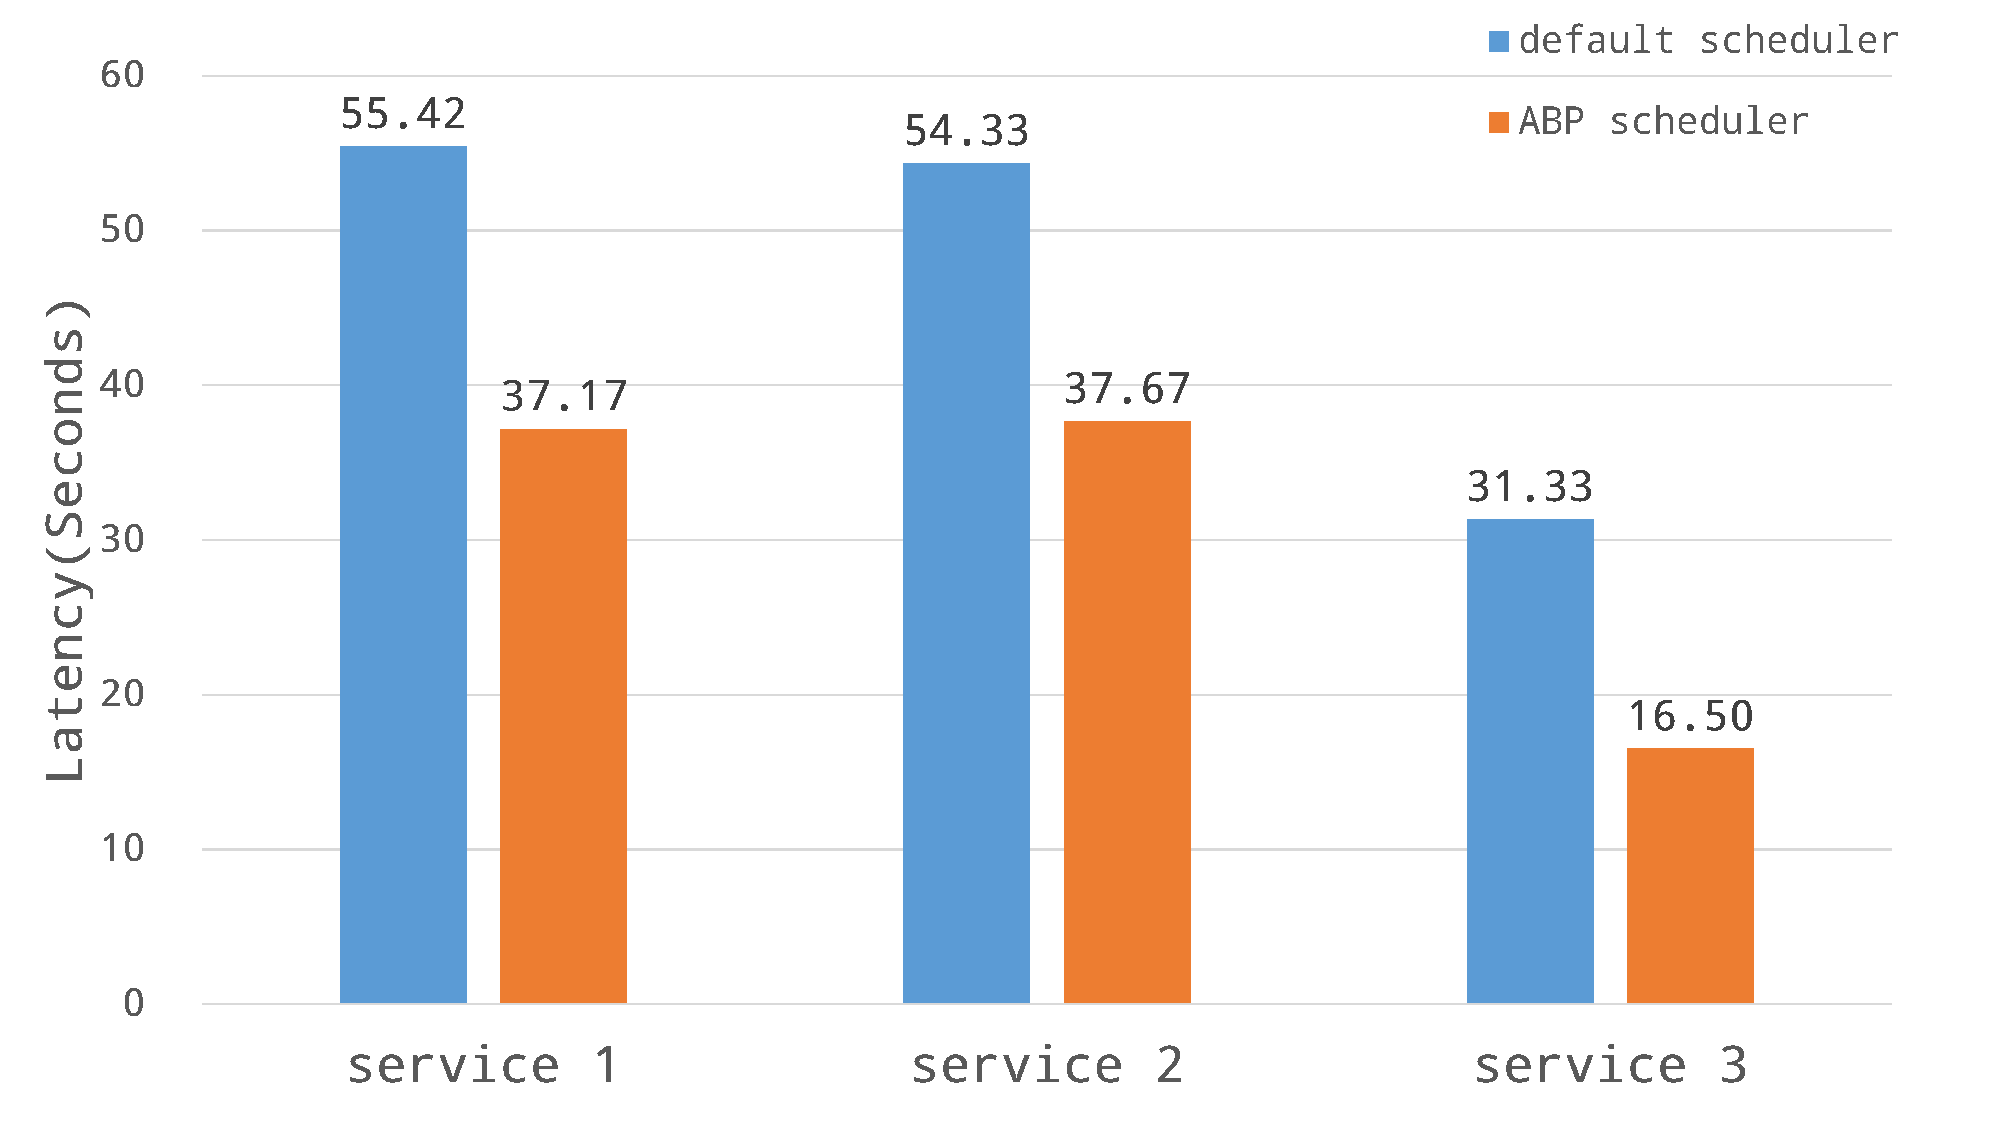
\includegraphics[width=0.9\textwidth]{./figure/4ins2rep}
\bicaption[fig:4ins]{创建服务:每个服务副本数要求为2且有4个任务实例}{\textbf{服务创建耗时}:每个服务副本数要求为2且有4个任务实例}{Fig}{\textbf{Services Creation}: creating each service with 4 tasks and 2 replicas}
\end{figure}

从图\ref{fig:4ins}中可知,在测试场景\ref{create2}下,服务在容器云中通过本课题提出的系统比通过Docker \emph{swarm}框架能以更快的速度完成创建和启动。对比图\ref{fig:4ins}和图\ref{fig:baseline},我们可以发现随着任务实例数的增加,Docker \emph{swarm}框架需要接近两倍于基准的延迟等待时间来完成相应服务的创建启动过程。Docker \emph{swarm}框架中服务启动出现大幅度延迟的原因是容器集群和本地Docker \emph{registry}镜像服务间的网络带宽。根据在之前的实验环境\ref{req:registry_mirror},容器集群和本地Docker \emph{registry}镜像服务间的网络带宽为100Mbps。在测试场景\ref{create2}下,每个服务在容器云中有4个任务实例需要创建并运行。在Docker \emph{swarm}框架下,每个服务的4个任务实例被平均分配到集群的4个节点上,集群内的网络请求数目随着实例数目增长而增长(最多可达到集群内的节点数目)。当这4个节点接受了对应的任务实例后,节点上的Docker Engine会开始从本地Docker \emph{registry}镜像服务获取相应的Docker镜像。在测试场景\ref{create1}下,由于每个服务只有2个任务实例,所以每次服务创建时只有两个镜像下载请求来平分容器集群和本地Docker \emph{registry}镜像服务间的网络带宽。在测试场景\ref{create2}中,因为有4个镜像下载请求同时存在,导致网络带宽由原来被2个下载请求平分变成被4个下载请求平分。网络请求数目增加了一倍,使得每个下载请求的传输速度只有测试场景\ref{create1}中的一半,导致整体下载耗时增加了一倍。与Docker \emph{swarm}框架相反,在本课题提出的系统中,为了满足服务自身的可用性目标,每个服务的4个任务实例被分配到了集群内的2个节点上。这使得系统在满足服务可用性要求的前提下,整个容器集群中只有两个节点发出下载请求使用网络。容器集群和本地Docker \emph{registry}镜像服务间的100Mbps网络带宽在实验场景\ref{create1}中和实验场景\ref{create2}中都是同时被两个下载请求平分,并没有增加集群内的网络流量。每个下载请求的传输速度没有变化,因此服务整体的启动延迟在实验场景\ref{create2}中和实验场景\ref{create1}中几乎一致。

\begin{figure}[htbp]
\centering
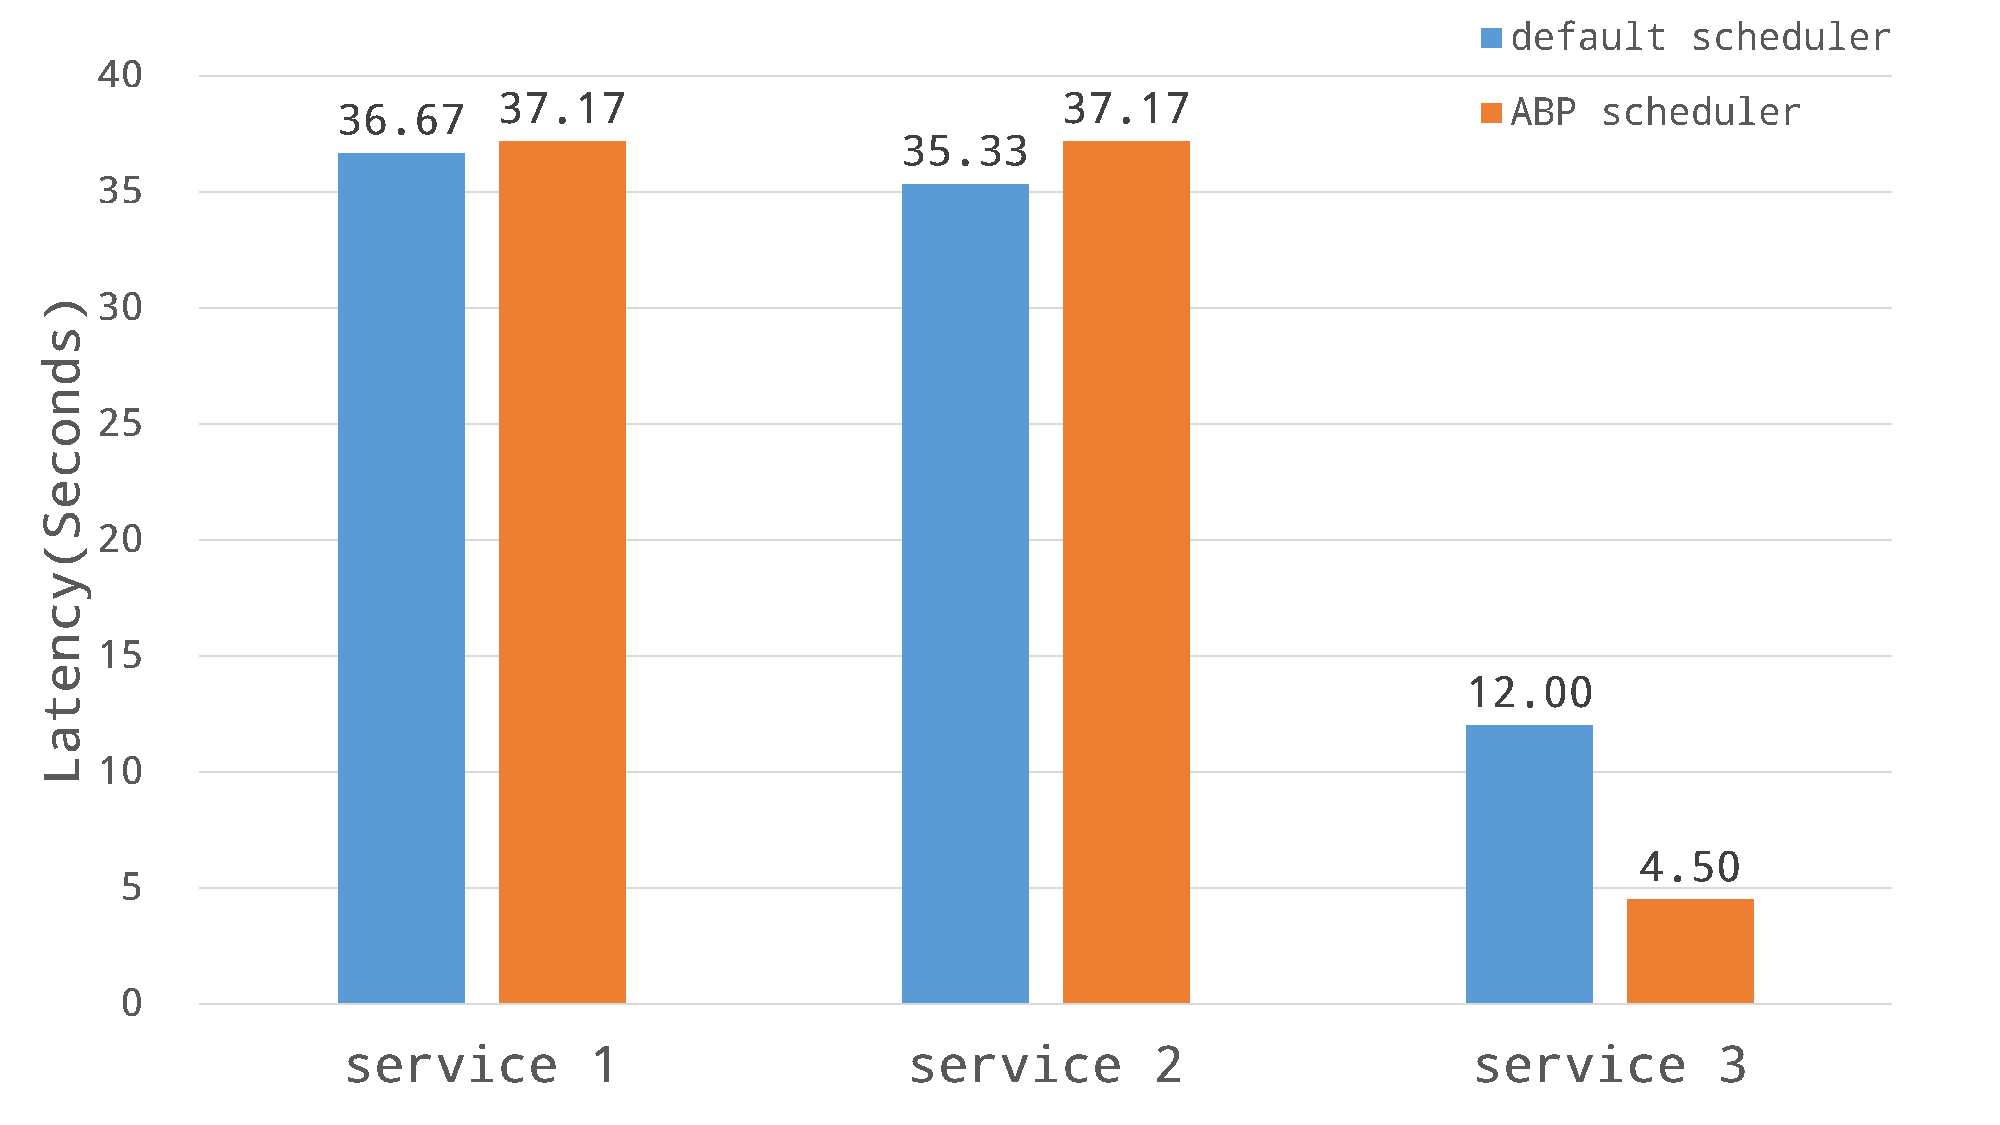
\includegraphics[width=0.9\textwidth]{./figure/132}
\bicaption[fig:132]{按照\emph{service1},\emph{service3}和\emph{service2}的顺序依次创建服务:每个服务副本数要求为2且有2个任务实例}{\textbf{服务创建耗时}: 每个服务副本数要求为2且有2个任务实例,按照\emph{service1},\emph{service3}和\emph{service2}的顺序依次创建各个服务}{Fig}{\textbf{Services Creation}: creating services with 2 tasks and 2 replicas in a sequence of \emph{service1}, \emph{service3} and \emph{service2}}
\end{figure}

服务用于满足自身可用性要求的副本数常常并不等于满足自身负载需求的实例数。在实际中,相比满足可用性目标的副本个数,服务往往需要更多的实例来应对自身的负载需要来保证服务本身的质量。为了评估本课题提出的系统在该场景下的表现,我们设计了实验场景\ref{create3}并进行了相关实验,实验结果如图\ref{fig:132}所示。从图\ref{fig:132}中可以明显看出,对比Docker \emph{swarm}框架,\emph{service3}整体的启动延迟时间在本课题提出的系统中显著降低。这主要是如我们在第\ref{chap:sys_design}章中所说,因为本课题提出的系统在资源分配阶段考虑了Docker镜像中的层级文件和容器集群节点上保存的Docker镜像文件缓存相关性,在同一节点上的不同服务间共享了部分Docker镜像分层文件缓存,降低了服务在创建和启动方面的延迟。根据我们在前面准备部分\ref{req:serv_image}中相关Docker镜像的具体构成,服务\emph{service1}和服务\emph{service3}使用的应用镜像\emph{image1}和\emph{image3}都包含了来自\emph{debian:jessie}这个基础镜像的同样的层级文件。在服务\emph{service1}被创建的过程中,\emph{debian:jessie}镜像的层级文件会被这些准备运行服务\emph{service1}相关任务实例的集群节点下载并缓存。在对服务\emph{service3}的任务实例基于负载应对选择托管的容器集群节点时,根据在\ref{sec:sec:node_selection}节中的设计,本课题提出的系统将优先把相应任务实例分布到那些已经运行了服务\emph{service1}任务实例的集群节点。在实验过程中,我们也发现如果按照\emph{service1}、\emph{service2}和\emph{service3}的顺序创建相关服务,服务\emph{service3}的任务实例在Docker \emph{swarm}框架下有时也会被分发到运行着服务\emph{service1}任务实例的集群节点上。这主要是当集群中节点运行的任务实例数目相同时,Docker \emph{swarm}框架根据节点的通用唯一识别码(Universally Unique Identifier,UUID)按照字典序进行任务的分发和调度,集群中节点的UUID则由节点上的Docker Engine在启动的时候基于sha256算法随机生成。

\subsection{服务伸缩实验}\label{sec:serv_scale}
我们已经在第\ref{sec:serv_creation}节中显示了本课题提出的系统在服务创建和启动方面相比Docker \emph{swarm}框架带来的显著提升。虽然服务创建的表现对保障服务质量很重要,但是在动态变化的负载压力下,服务进行伸缩的性能表现则是关键。当负载增长时,服务需要进行扩展(scale-out)以保证服务质量;当负载降低时,服务需要进行收缩(scale-in)从而减少不必要的资源,提高资源使用率,降低成本。降低服务伸缩过程任务实例的启动/关闭延迟可以增强服务整体应对负载的灵活性,从而更好地保证服务的质量。为了验证本课题提出的系统在服务扩展和服务收缩场景下对任务实例启动延迟的影响,我们设计了如下两个实验并和Docker \emph{swarm}框架进行了对比:

\begin{enumerate}
\item\label{scale1} 基于服务创建实验\ref{create1}中的要求创建服务,然后将相应的服务扩展到4个任务实例,最后再将相应服务收缩到2个任务实例。对服务\emph{service1},\emph{service2}和\emph{service3}独立进行上述实验,每次实验之前重置整个实验环境,保证不同服务的实验之间没有影响。
\item\label{scale2} 基于服务创建实验\ref{create3}创建服务,分别用Docker \emph{swarm}和本文提出的系统按照\emph{service1},\emph{service3}和\emph{service2}的顺序依次创建服务。每个服务有2个任务实例,同时为了满足\ref{req:serv_aval}中提到的可用性要求,在本课题提出的系统中为每个服务设置2个副本。随后,将服务\emph{service1}扩展到4个任务实例。
\end{enumerate}

以上两个实验设计均包含了服务的扩展和伸缩部分,但是这两个设计针对的场景侧重点不同。实验设计场景\ref{scale1}主要通过对各个服务的伸缩性能进行独立实验来验证本系统在单一服务场景下对单个服务伸缩性能的影响;验设计场景\ref{scale2}通过从所有服务中选择一个服务来进行伸缩实验从而来验证本系统在多服务的场景下对其中一个服务进行伸缩时的性能影响。以下将根据以上两个设计场景下的实验结果整合后,分为服务扩展和服务收缩两部分进行介绍和说明。

\subsubsection{服务扩展表现}\label{sec:scaleout}

\begin{figure}[htbp]
\centering
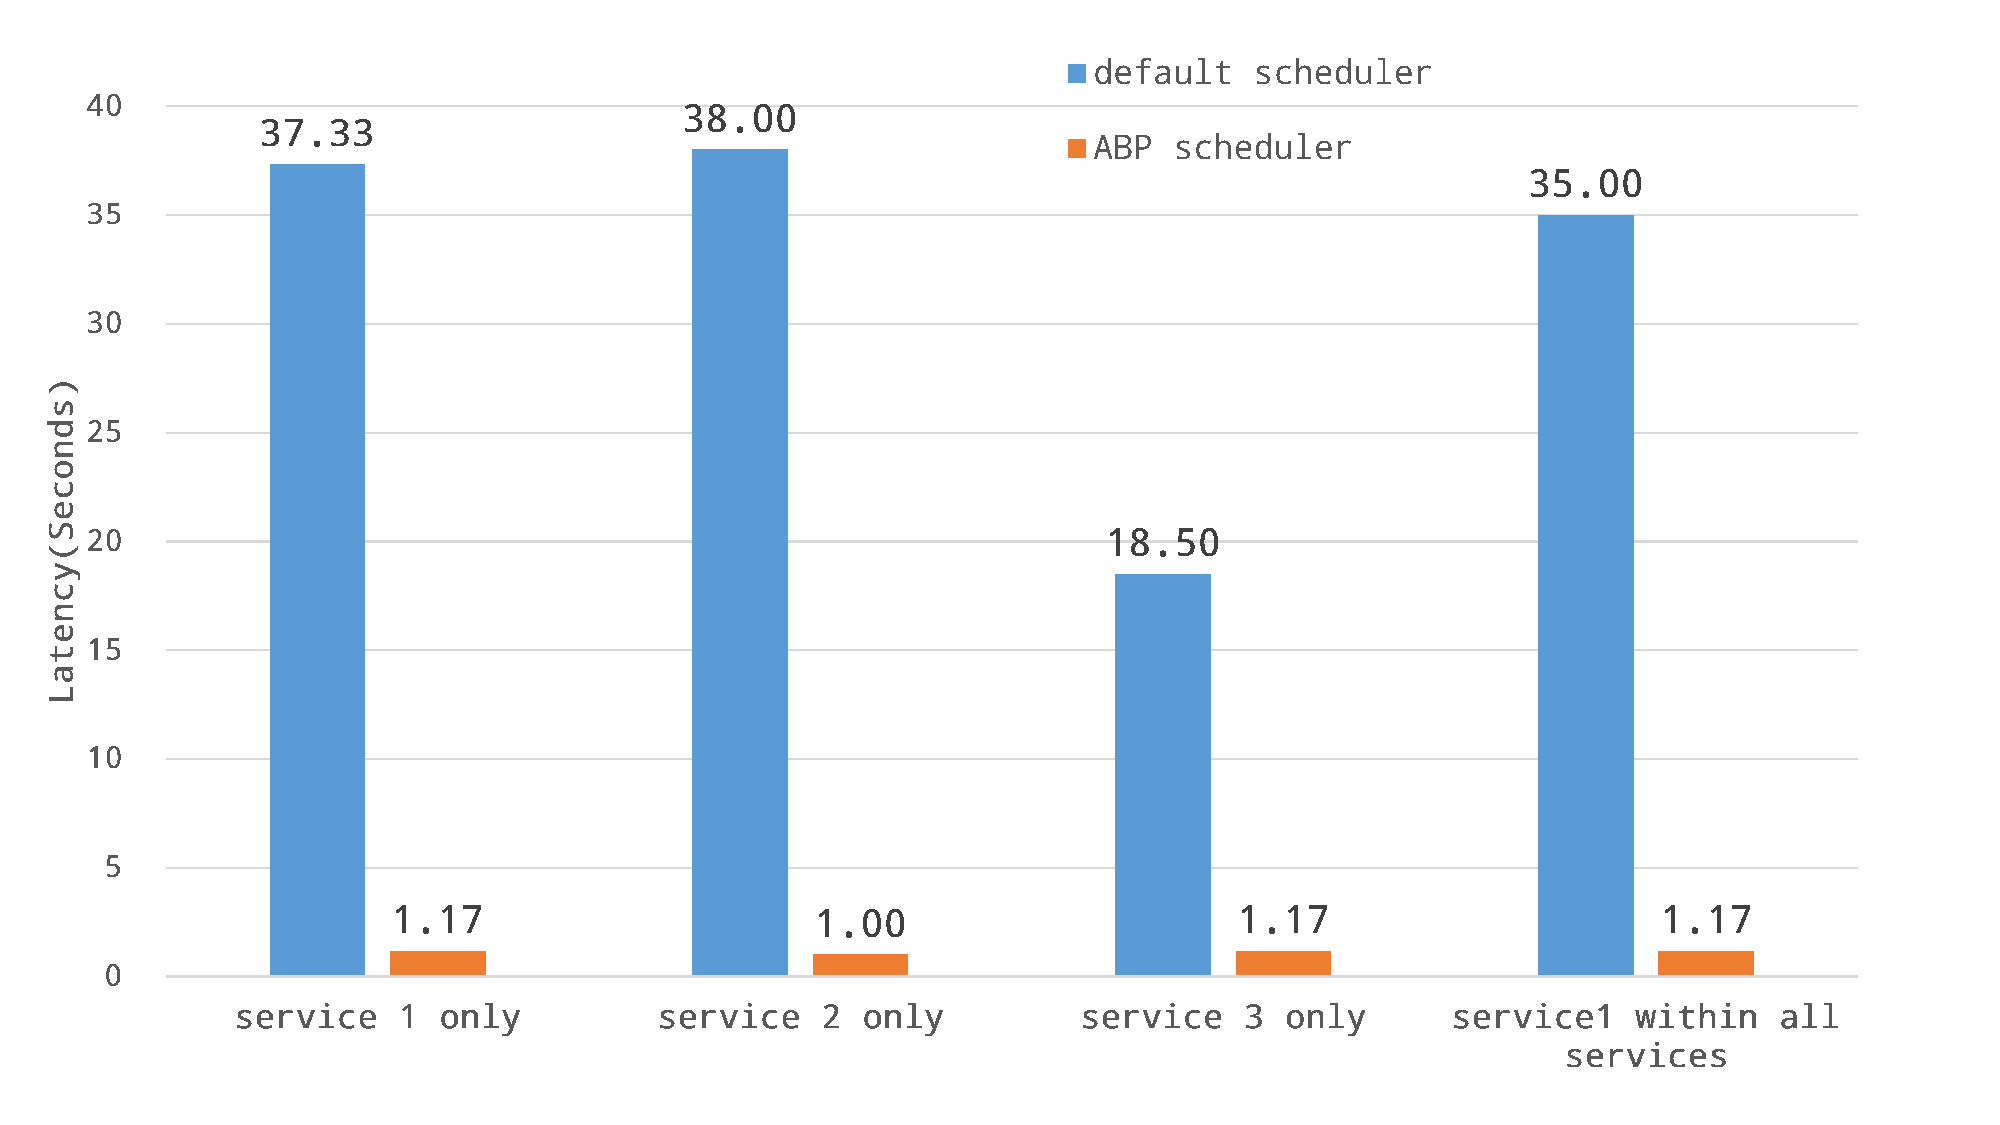
\includegraphics[width=0.9\textwidth]{./figure/scaleout}
\bicaption[fig:scaleout]{服务扩展}{\textbf{服务扩展-应对负载增加}}{Fig}{Service Scaling Out}
\end{figure}

图\ref{fig:scaleout}展示了服务扩展操作在本课题提出的系统中有一个显著的加速,服务整体的扩展延迟比在Docker \emph{swarm}框架中有大幅度降低。通过本课题提出的系统,容器集群中的服务能在极短的延迟(基本不超过2s)下完成伸缩,这显然在负载急剧增长的场景下能对提升服务整体的服务质量有极大的帮助。与之相对,我们发现在Docker \emph{swarm}框架下,每个服务的扩展延迟几乎等于他们创建阶段的耗时,而创建耗时又和服务所使用的Docker镜像大小密切相关。鉴于Docker \emph{swarm}框架中服务的任务实例常常被尽可能平均地分发到了整个容器集群中所有满足限制条件的节点上,使得整个容器集群中的节点上任务实例近似一致。而在整个容器集群中,并不是所有节点都拥有相应服务所依赖的层级文件缓存。这就导致有些任务实例被分发到了一个完全没有任何相关依赖层级文件缓存的集群节点上,而这些节点则需要下载对应服务所需要的完整Docker镜像从而来运行这些任务实例。当服务在本课题提出的系统中需要进行扩展的时候,系统会根据节点上的层级文件缓存和当前服务所需Docker镜像中层级文件的重合度以及节点的资源利用率来从容器集群中选择合适的节点来运行扩展的任务实例。因此在系统中被选择用作运行新任务实例的节点不需要下载全部的Docker镜像文件,加快了扩展任务实例的启动时间,从而降低了服务扩展操作的整体延时。

针对伸缩实验场景\ref{scale2},我们从图\ref{fig:scaleout}中还可以发现:按照\emph{service1},\emph{service3}和\emph{service2}的顺序创建相应服务后,在Docker \emph{swarm}框架下对服务\emph{service1}进行扩展的时候服务扩展所需要的耗时相比单独对服务\emph{service1}进行扩展时所要的耗时降低了一点。造成这个现象的原因是在该场景下容器集群中所有节点都有了底层基础镜像\emph{debian:jessie}镜像的层级文件缓存从而减少了这部分文件下载所需要的耗时。在该场景下,由于集群只有4个节点并且服务按照\emph{service1}、\emph{service3}和\emph{service2}的顺序依次创建,服务\emph{service1}扩展产生的任务实例被分发到集群中尚未运行服务\emph{service1}任务实例的两个节点。我们在之前准备环境\ref{req:serv_image}部分中已经说明了服务\emph{service1}和服务\emph{service3}使用的应用镜像\emph{image1}和\emph{image3}由于都使用\emph{debian:jessie}镜像作为基础镜像,因此这两个应用镜像共享这部分的层级文件。因此在对服务\emph{service1}进行扩展的时候,这两个节点上已经运行了服务\emph{service3}的相关任务实例,因此针对\emph{debian:jessie}镜像这一部分的层级文件可以直接利用存储在各自节点上的缓存而不需要再次下载。不过我们从图\ref{fig:scaleout}中也可以发现,即使利用了这部分缓存的共享层级文件,对服务扩展操作的加速仍然只是杯水车薪。在Docker \emph{swarm}框架中,运行扩展任务实例的节点仍然需要下载约270MB大小的层级文件以安装应用运行所需要的\emph{Golang}运行时环境。与之相对,在本课题提出的系统中,运行扩展任务实例的节点由于在本地已经缓存了服务\emph{service1}使用的Docker容器镜像,因此避免了对相应层级文件的下载耗时和网络开销。

\subsubsection{服务收缩表现}\label{sec:scalein}

当服务在Docker \emph{swarm}框架中进行收缩时,Docker \emph{swarm}框架会从所有节点中根据运行该服务相应任务实例数目进行选择并试图将集群中节点上运行的实例数目接近一致。在相同场景下,如我们在之前的设计章节%\ref{algo:scalein}
中所说,本课题提出的系统则根据任务实例的优势资源相对节点总资源的占比进行选择。

\begin{figure}[htbp]
\centering
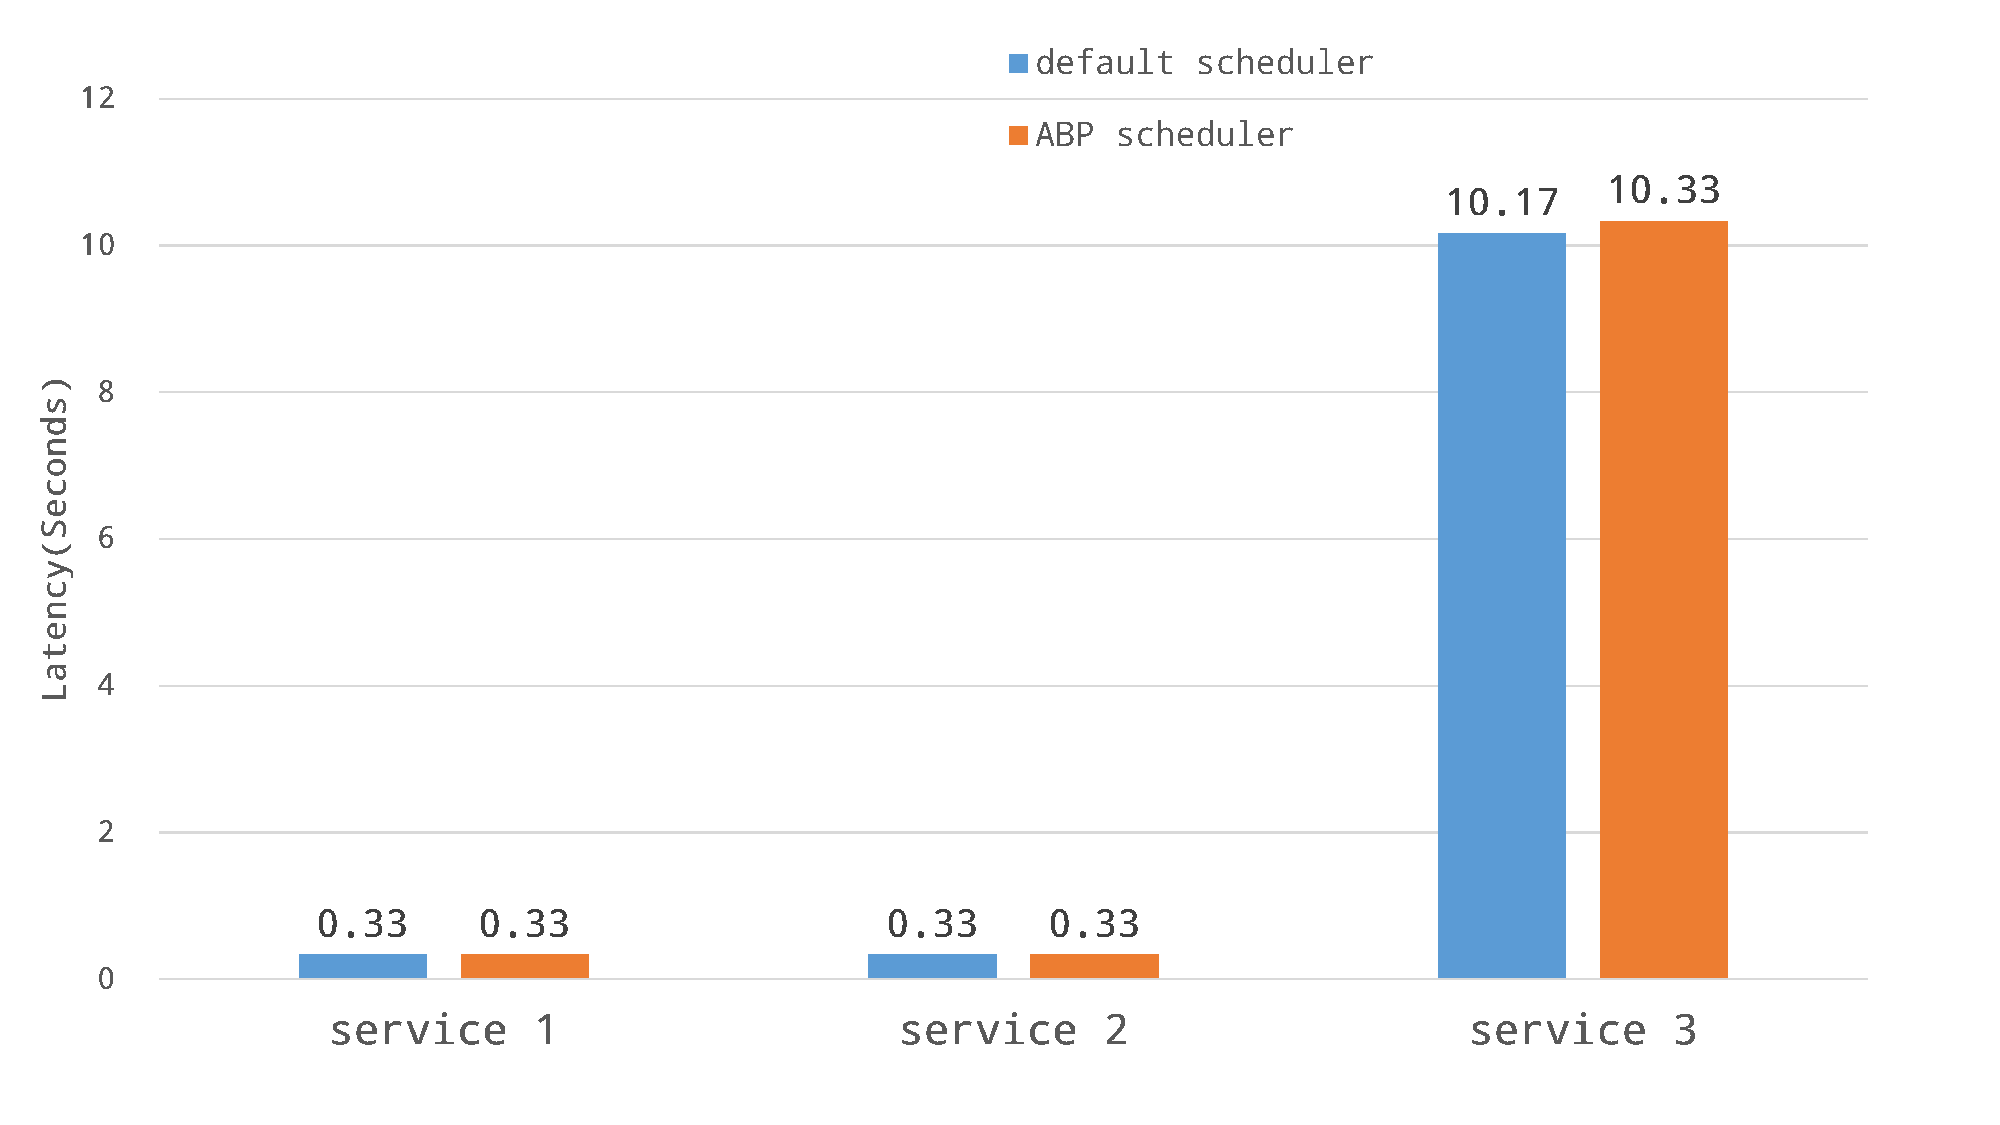
\includegraphics[width=0.9\textwidth]{./figure/scalein}
\bicaption[fig:scalein]{服务收缩}{\textbf{服务收缩-应对负载降低}}{Fig}{Service Scaling In}
\end{figure}

图\ref{fig:scalein}显示了服务收缩在Docker \emph{swarm}框架和本课题提出的系统中所需要的延迟时间。我们由图\ref{fig:scalein}可以发现服务在Docker \emph{swarm}框架和本课题提出的系统中几乎都是立即完成了相应的服务收缩操作,收缩操作的时间延迟基本不超过0.5秒。服务\emph{service3}的收缩操作延迟相比其他两个服务显得很异常,但是也这是在预期之中的。这主要是因为服务\emph{service3}运行的是一段包含了无限循环的shell脚本,导致运行相应任务实例的容器无法响应该节点上的Docker Engine正常发送的停止请求。根据Docker Engine中定义的容器关闭规则,在经过一个既定的等待期(默认10秒)之后,Docker Engine将通过发送SIGKILL的方式强制杀死运行对应任务实例的容器进程。通过对比,我们可以发现服务在Docker \emph{swarm}框架和本课题提出的系统中进行收缩需要的延迟几乎毫无差别。

\section{本章小结}
在本章中,我们从负载预测的准确性和新任务实例调度策略对容器云中任务实例分发管理的影响
%本章就我们对本文提出的云环境下需求驱动的动态资源调度框架的系统验证工作进行讨论。为了反映出框架的真实有效性,我们在真实的云环境部署了真实的云应用,令框架完成云环境下的各类资源调度活动。实验证明,该框架能够在保障云应用提供商与云应用用户约定的SLA 的约束下,弹性地对云应用进行虚拟机资源的供给;同时,框架还能够在兼顾云应用可用性及虚拟机之间通讯开销的情况下,为云应用进行虚拟机资源的安置;此外,框架还能够从云资源提供商的角度出发,通过虚拟机资源整合活动提高物理基础设施的资源利用率同时避免物理机过载。
本章通过使用98 年世界杯期间的负载情况模拟了多种类型的用户请求,对比了面对突发流量变化时,本文所提出的动态资源管理方案与其它一些已有的解决方案。通过对实验结果的分析,本文所提出的方案在面对突发流量增长时,可以提前感知并扩展充足的资源给当前程序,从而保证了程序在面对突发流量增长时的可用性;本文提出的方案在面对流量的快速下降时,也可以选择合适的时机回收过多分配的资源,从而实现了高成本效益目标。与此同时,由于结合了垂直扩展和水平扩展的优点,相比一些已有的研究方案而言,本文的方案能更快地完成伸缩操作,从而显著降低了面对突发流量变化时的时间延迟。

%# -*- coding: utf-8-unix -*-
%%==================================================
%% conclusion.tex for SJTUThesis
%% Encoding: UTF-8
%%==================================================
\chapter{总结和展望}\label{chap:summary}
\section{全文总结}
得益于容器虚拟化技术的轻便,越来越多的用户正逐渐转向容器云相关服务。但是对于云服务而言,仅仅是容器本身轻便带来的帮助还是有限的。特别是在负载变化的场景下,用户需要通过调整服务的实例规模来应对负载的变化,保证自身的服务质量;容器云服务提供商需要提高整体资源使用率,从而降低云服务的成本。降低云服务中服务实例的创建和扩展延迟对提升云服务中的服务启动和伸缩速度,从而提高服务应对负载变化的灵活性,对保障服务质量和降低云服务成本有重要意义。

虽然容器本身相比传统的虚拟机而言更加轻量,能在更短时间内创建更多的容器实例,但是目前已有的容器云在服务的创建和伸缩方面,尤其是扩展方面表现仍然不够理想。除此之外,现有的容器集群管理框架中缺少对服务的副本数进行合理的定义,将服务的实例数兼用作服务的副本数,对保障服务的可用性目标造成很大的干扰。因此本课题提出了一个基于可用性模型的主动式容器云资源管理模型,在保证服务可用性目标的前提下加速容器云中服务的创建和伸缩性能,使得容器云中的服务能更好地应对负载的变化。

本文将资源使用状态作为负载的衡量手段,从CPU、内存和网络带宽等资源类型对服务和集群节点的资源使用状态进行周期性监测。随后根据监测获得的历史数据,我们分别使用基于整合移动平均自回归模型的预测算法和基于长短期记忆模型的预测算法对资源使用状态进行预测。根据历史记录对接下来的资源使用状态进行预测来提前获知接下来的负载变化趋势,从而提前主动做出相应调整,使得后续只需要根据实际的负载状态对服务规模进行轻微调整,从而加强了系统应对负载变化的灵活性。

本文以容器云中服务实例分布的集群节点作为服务的副本构建容器云中服务的可用性模型,以服务实例分布的节点数来表征服务的可用性,通过控制服务在容器云中节点的分布情况来满足服务的可用性要求。本文通过引入副本数,结合资源监测和预测的资源使用状态,在资源供给和优化模块中确认满足实际负载需求所需要的任务实例数。资源管理模块利用Docker \emph{Registry} API获取运行相关服务所需Docker镜像的元信息,并通过引入新的接口来获取容器云中各节点上全部的Docker镜像层间文件缓存状态。最后,负载优化模块根据运行服务所需的Docker镜像信息和容器云上的层级文件缓存状态,基于启发式的多优先级比较规则确认最终的任务实例调度选择。

我们通过实验对本文提出的模型分别就资源使用状态预测和服务的创建与伸缩这两个方面进行验证。实验结果显示基于该模型实现的系统对服务在容器集群中的创建和伸缩性能有显著提高,在满足服务可用性要求的前提下,相比Docker swarm框架大幅降低了服务创建和服务扩展的延迟。

\section{不足与展望}
尽管我们基于本课题提出的模型实现的资源管理系统显著加速了容器云中服务的启动和伸缩过程,但是由于实际中云服务的复杂性和容器本身尚未达成一致的商业化标准,该模型和我们基于该模型实现的系统仍然有很多改进的空间:
\begin{enumerate}
\item 系统目前只支持基于整合移动平均自回归平均模型的预测算法实现和基于长短期记忆模型的预测算法实现,为了进一步提高负载预测的精度,可以引入诸如GARCH等其他预测算法和模型,并在此基础之上对这些算法进行优化,提升最终的预测准确度和稳定性。
\item 目前的模型假定集群中所有节点的可用性都是一样的,而在现实中集群内各节点的可用性指标必然不是全部一致的。因此在未来,我们需要针对由不同可用性指标的节点组成的容器云提出相应的可用性计算模型,从而得到在该场景下服务满足自身可用性目标所需要的副本数目。
\item 目前模型以\emph{REST API}的方式从Docker \emph{registry}服务获取Docker镜像中相应层级文件的数字摘要,从而计算Docker镜像和容器集群中节点上缓存的一致性。然而这些层级文件的数字摘要是基于Docker \emph{registry}服务上压缩过的层级文件生成的。这就使得相比基于未压缩的层级文件生成的数字摘要而言,目前不同层级文件的数字摘要之间出现冲突的可能性更大。因此,我们需要针对Docker \emph{registry}服务设计一个新的\emph{REST API}用来获取基于未压缩的层级文件生成的数字摘要。
\item 我们当前的系统是基于Docker \emph{swarm}实现的,后续可以将该模型应用到诸如Kubernetes和Mesos等其他容器集群管理框架中,构建相应的主动式容器云管理系统。
\end{enumerate}


\appendix	% 使用英文字母对附录编号,重新定义附录中的公式、图图表编号样式
\renewcommand\theequation{\Alph{chapter}--\arabic{equation}}	
\renewcommand\thefigure{\Alph{chapter}--\arabic{figure}}
\renewcommand\thetable{\Alph{chapter}--\arabic{table}}
\renewcommand\thealgorithm{\Alph{chapter}--\arabic{algorithm}}

%% 附录内容,本科学位论文可以用翻译的文献替代。
% \include{tex/app_setup}
% \include{tex/app_eq}
% \include{tex/app_cjk}
% \include{tex/app_log}

\backmatter	% 文后无编号部分 

%% 参考资料
\printbibliography[heading=bibintoc]

%% 致谢、发表论文、申请专利、参与项目、简历
%% 用于盲审的论文需隐去致谢、发表论文、申请专利、参与的项目
\makeatletter

%%
% "研究生学位论文送盲审印刷格式的统一要求"
% http://www.gs.sjtu.edu.cn/inform/3/2015/20151120_123928_738.htm

% 盲审删去删去致谢页
\ifsjtu@review\relax\else
  %# -*- coding: utf-8-unix -*-
\begin{thanks}
两年半的研究生生涯即将终结,在这段求学的日子里,我在学术研究和为人处世方面从各位老师和同学身上学到很多。很荣幸能够借这个机会,向往日里给予我关心和帮助的他们表示感谢!

首先要感谢在我读研期间负责指导我的陈昊鹏老师。陈老师不仅在学术研究方面对我进行了耐心细致的指导,在日常生活中也给予我关心和鼓励,通过言传身教的方式教会了我很多人生道理,在此谨向陈昊鹏老师表示最真挚的敬意和感谢。

其次要感谢实验室的同学们在这段研究生求学期间的陪伴和帮助。如果在过去两年多的时间中没有和实验室的大家相遇相知,我相信我的研究生生活相比现在一定要褪色不少。

最后我要感谢我的家人。正是由于你们在我研究生求学期间对我的默默支持与帮助,我才能顺利完成学业,感谢你们一直以来对我的陪伴和支持。
\end{thanks}
 	  %% 致谢
\fi

\ifsjtu@bachelor
  % 学士学位论文要求在最后有一个英文大摘要,单独编页码
  \pagestyle{biglast}
  %# -*- coding: utf-8-unix -*-
\begin{bigabstract}

\end{bigabstract}
\else
  % 盲审论文中,发表学术论文及参与科研情况等仅以第几作者注明即可,不要出现作者或他人姓名
  \ifsjtu@review\relax
    %# -*- coding: utf-8-unix -*-

\begin{publications}{99}
    \item\textsc{第一作者}. {IEEE国际会议论文}, 2017.
\end{publications}

    \include{tex/projectsreview}  
  \else
    %# -*- coding: utf-8-unix -*-
%%==================================================
%% pub.tex for SJTUThesis
%% Encoding: UTF-8
%%==================================================

\begin{publications}{99}
    \item\textsc{Ye Wu, Haopeng Chen}. {ABP Scheduler: Speeding up Service Spread inDocker swarm}[C]]//Parallel and Distributed Processing with Applications (ISPA), 2017 IEEE International Symposium on. IEEE, 2017: 691-698.
\end{publications}
	      %% 发表论文
    \include{tex/projects}  %% 参与的项目
  \fi
\fi

% \include{tex/patents}	  %% 申请专利
% \include{tex/resume}	  %% 个人简历

\makeatother

\end{document}
